% Judul dokumen
\title{Buku Tugas Akhir ITS}
\author{Fajri, Dimas Aditya Maulana}

% Pengaturan ukuran teks dan bentuk halaman dua sisi
\documentclass[12pt,twoside]{report}

% Pengaturan ukuran halaman dan margin
\usepackage[a4paper,top=30mm,left=30mm,right=20mm,bottom=25mm]{geometry}

% Pengaturan ukuran spasi
\usepackage[singlespacing]{setspace}

% Pengaturan detail pada file PDF
\usepackage[pdfauthor={\@author},bookmarksnumbered,pdfborder={0 0 0}]{hyperref}

% Pengaturan jenis karakter
\usepackage[utf8]{inputenc}

% Pengaturan pewarnaan
\usepackage[table,xcdraw]{xcolor}

% Pengaturan kutipan artikel
\usepackage[style=apa, backend=biber]{biblatex}

% Package lainnya
\usepackage{changepage}
\usepackage{enumitem}
\usepackage{eso-pic}
\usepackage{txfonts} % Font times
\usepackage{etoolbox}
\usepackage{graphicx}
\usepackage{lipsum}
\usepackage{longtable}
\usepackage{tabularx}
\usepackage{wrapfig}
\usepackage{float}
\usepackage{multirow}
\usepackage{fixltx2e}


% Definisi untuk "Hati ini sengaja dikosongkan"
\patchcmd{\cleardoublepage}{\hbox{}}{
  \thispagestyle{empty}
  \vspace*{\fill}
  \begin{center}\textit{[Halaman ini sengaja dikosongkan]}\end{center}
  \vfill}{}{}

% Pengaturan penomoran halaman
\usepackage{fancyhdr}
\fancyhf{}
\renewcommand{\headrulewidth}{0pt}
\pagestyle{fancy}
\fancyfoot[LE,RO]{\thepage}
\patchcmd{\chapter}{plain}{fancy}{}{}
\patchcmd{\chapter}{empty}{plain}{}{}

% Command untuk bulan
\newcommand{\MONTH}{%
  \ifcase\the\month
  \or Januari% 1
  \or Februari% 2
  \or Maret% 3
  \or April% 4
  \or Mei% 5
  \or Juni% 6
  \or Juli% 7
  \or Agustus% 8
  \or September% 9
  \or Oktober% 10
  \or November% 11
  \or Desember% 12
  \fi}
\newcommand{\ENGMONTH}{%
  \ifcase\the\month
  \or January% 1
  \or February% 2
  \or March% 3
  \or April% 4
  \or May% 5
  \or June% 6
  \or July% 7
  \or August% 8
  \or September% 9
  \or October% 10
  \or November% 11
  \or December% 12
  \fi}

% Pengaturan format judul bab
\usepackage{titlesec}
\titleformat{\chapter}[display]{\bfseries\Large}{BAB \centering\Roman{chapter}}{0ex}{\vspace{0ex}\centering}
\titleformat{\section}{\bfseries\large}{\MakeUppercase{\thesection}}{1ex}{\vspace{1ex}}
\titleformat{\subsection}{\bfseries\large}{\MakeUppercase{\thesubsection}}{1ex}{}
\titleformat{\subsubsection}{\bfseries\large}{\MakeUppercase{\thesubsubsection}}{1ex}{}
\titlespacing{\chapter}{0ex}{0ex}{4ex}
\titlespacing{\section}{0ex}{1ex}{0ex}
\titlespacing{\subsection}{0ex}{0.5ex}{0ex}
\titlespacing{\subsubsection}{0ex}{0.5ex}{0ex}

% Atur variabel berikut sesuai namanya

% nama
\newcommand{\name}{Dimas Aditya Maulana Fajri}
\newcommand{\authorname}{Fajri, Dimas Aditya Maulana}
\newcommand{\nickname}{Dimas}
\newcommand{\advisor}{Arief Kurniawan, S.T., M.T.}
\newcommand{\coadvisor}{Dr. Eko Mulyanto Yuniarno, S.T., M.T.}
\newcommand{\examinerone}{Penguji 1}
\newcommand{\examinertwo}{Penguji 2}
\newcommand{\examinerthree}{Penguji 2}
\newcommand{\headofdepartment}{Dr. Supeno Mardi Susiki Nugroho, S.T., M.T}

% identitas
\newcommand{\nrp}{0721 19 4000 0012}
\newcommand{\advisornip}{19740907 200212 1 001}
\newcommand{\coadvisornip}{19680601 199512 1 009}
\newcommand{\examineronenip}{-}
\newcommand{\examinertwonip}{-}
\newcommand{\examinerthreenip}{-}
\newcommand{\headofdepartmentnip}{19700313 199512 1 001}

% judul
\newcommand{\tatitle}{PREDIKSI JUMLAH KALORI YANG TERBAKAR SAAT BEROLAHRAGA DENGAN TREADMILL BERBASIS KAMERA MENGGUNAKAN \emph{CONVOLUTIONAL NEURAL NETWORK}}
%\newcommand{\tatitle}{PREDIKSI JUMLAH KALORI YANG TERBAKAR SAAT BEROLAHRAGA DENGAN TREADMILL BERBASIS KAMERA MENGGUNAKAN CNN}
\newcommand{\engtatitle}{\emph{PREDICTION OF CALORIES BURNED WHEN EXERCISING ON A TREADMILL WITH CAMERA-BASED USING A CONVOLUTIONAL NEURAL NETWORK}}

% tempat
\newcommand{\place}{Surabaya}

% jurusan
\newcommand{\studyprogram}{Teknik Komputer}
\newcommand{\engstudyprogram}{Computer Engineering}

% fakultas
\newcommand{\faculty}{Teknologi Elektro dan Informatika Cerdas}
\newcommand{\engfaculty}{Intelligent Electrical and Informatics Technology}

% singkatan fakultas
\newcommand{\facultyshort}{FTEIC}
\newcommand{\engfacultyshort}{ELECTICS}

% departemen
\newcommand{\department}{Teknik Komputer}
\newcommand{\engdepartment}{Computer Engineering}

% kode mata kuliah
\newcommand{\coursecode}{EC224801}


% Tambahkan format tanda hubung yang benar di sini
\hyphenation{
  ro-ket
  me-ngem-bang-kan
  per-hi-tu-ngan
}

% Menambahkan resource daftar pustaka
\addbibresource{pustaka/pustaka.bib}

% Pengaturan format potongan kode
\usepackage{listings}
\definecolor{comment}{RGB}{0,128,0}
\definecolor{string}{RGB}{255,0,0}
\definecolor{keyword}{RGB}{0,0,255}
\lstdefinestyle{codestyle}{
  commentstyle=\color{comment},
  stringstyle=\color{string},
  keywordstyle=\color{keyword},
  basicstyle=\footnotesize\ttfamily,
  numbers=left,
  numberstyle=\tiny,
  numbersep=5pt,
  frame=lines,
  breaklines=true,
  prebreak=\raisebox{0ex}[0ex][0ex]{\ensuremath{\hookleftarrow}},
  showstringspaces=false,
  upquote=true,
  tabsize=2,
}
\lstset{style=codestyle}

% Isi keseluruhan dokumen
\begin{document}

% Sampul luar Bahasa Indonesia
\newcommand\covercontents{sampul/konten-id.tex}
\AddToShipoutPictureBG*{
  \AtPageLowerLeft{
    % Ubah nilai berikut jika posisi horizontal background tidak sesuai
    \hspace{-3.25mm}

    % Ubah nilai berikut jika posisi vertikal background tidak sesuai
    \raisebox{0mm}{
      
\includegraphics[width=\paperwidth,height=\paperheight]{sampul/gambar/sampul-luar-tipis.png}
    }
  }
}

% Menyembunyikan nomor halaman
\thispagestyle{empty}

% Pengaturan margin untuk menyesuaikan konten sampul
\newgeometry{
  top=65mm,
  left=30mm,
  right=30mm,
  bottom=20mm
}

\begin{flushleft}

  % Pemilihan font sans serif
  \sffamily

  % Pemilihan font bold
  \fontseries{bx}
  \selectfont
  \begin{spacing}{1.5}
    \input{\covercontents}
  \end{spacing}

\end{flushleft}

\restoregeometry


% Atur ulang penomoran halaman
\setcounter{page}{1}

% Sampul dalam Bahasa Indonesia
\renewcommand\covercontents{sampul/konten-id.tex}
\AddToShipoutPictureBG*{
  \AtPageLowerLeft{
    % Ubah nilai berikut jika posisi horizontal background tidak sesuai
    \hspace{-4mm}

    % Ubah nilai berikut jika posisi vertikal background tidak sesuai
    \raisebox{0mm}{
      
\includegraphics[width=\paperwidth,height=\paperheight]{sampul/gambar/sampul-luar-tipis.png}
    }
  }
}

% Menyembunyikan nomor halaman
\thispagestyle{empty}

% Pengaturan margin untuk menyesuaikan konten sampul
\newgeometry{
  top=65mm,
  left=30mm,
  right=30mm,
  bottom=20mm
}

\begin{flushleft}

  % Pemilihan font sans serif
  \sffamily

  % Pemilihan font bold
  \fontseries{bx}
  \selectfont
  \begin{spacing}{1.5}
    \input{\covercontents}
  \end{spacing}

\end{flushleft}

\restoregeometry

\clearpage
\cleardoublepage

% Sampul dalam Bahasa Inggris
\renewcommand\covercontents{sampul/konten-en.tex}
\AddToShipoutPictureBG*{
  \AtPageLowerLeft{
    % Ubah nilai berikut jika posisi horizontal background tidak sesuai
    \hspace{-4mm}

    % Ubah nilai berikut jika posisi vertikal background tidak sesuai
    \raisebox{0mm}{
      
\includegraphics[width=\paperwidth,height=\paperheight]{sampul/gambar/sampul-luar-tipis.png}
    }
  }
}

% Menyembunyikan nomor halaman
\thispagestyle{empty}

% Pengaturan margin untuk menyesuaikan konten sampul
\newgeometry{
  top=65mm,
  left=30mm,
  right=30mm,
  bottom=20mm
}

\begin{flushleft}

  % Pemilihan font sans serif
  \sffamily

  % Pemilihan font bold
  \fontseries{bx}
  \selectfont
  \begin{spacing}{1.5}
    \input{\covercontents}
  \end{spacing}

\end{flushleft}

\restoregeometry

\cleardoublepage

% Label tabel dan gambar dalam bahasa indonesia
\renewcommand{\figurename}{Gambar}
\renewcommand{\tablename}{Tabel}

% Pengaturan ukuran indentasi paragraf
\setlength{\parindent}{2em}

% Pengaturan ukuran spasi paragraf
\setlength{\parskip}{1ex}

% Lembar pengesahan
\begin{center}
  \large
  \textbf{LEMBAR PENGESAHAN}
\end{center}

% Menyembunyikan nomor halaman
\thispagestyle{empty}

\begin{center}
  \textbf{\tatitle{}}
\end{center}

\begingroup
% Pemilihan font ukuran small
\small

\begin{center}
  \textbf{TUGAS AKHIR}
  \\Diajukan untuk memenuhi salah satu syarat
  memperoleh gelar Sarjana Teknik pada \\
  Program Studi S-1 \studyprogram{} \\
  Departemen \department{} \\
  Fakultas \faculty{} \\
  Institut Teknologi Sepuluh Nopember
\end{center}

\begin{center}
  Oleh: \textbf{\name{}}
  \\NRP. \nrp{}
\end{center}

\begin{center}
  Disetujui oleh Tim Penguji Tugas Akhir:
\end{center}

\begingroup
% Menghilangkan padding
\setlength{\tabcolsep}{0pt}

\noindent
\begin{tabularx}{\textwidth}{X l}
  \advisor{}               & (Pembimbing I)                      \\
  NIP: \advisornip{}       &                                     \\
                           & ................................... \\
                           &                                     \\
                           &                                     \\
  \coadvisor{}             & (Pembimbing II)                     \\
  NIP: \coadvisornip{}     &                                     \\
                           & ................................... \\
                           &                                     \\
                           &                                     \\
  \examinerone{}.          & (Penguji I)                         \\
  NIP: \examineronenip{}   &                                     \\
                           & ................................... \\
                           &                                     \\
                           &                                     \\
  \examinertwo{}.          & (Penguji II)                        \\
  NIP: \examinertwonip{}   &                                     \\
                           & ................................... \\
                           &                                     \\
                           &                                     \\
  \examinerthree{}.        & (Penguji III)                       \\
  NIP: \examinerthreenip{} &                                     \\
                           & ................................... \\
\end{tabularx}
\endgroup

\begin{center}
  Mengetahui, \\
  Kepala Departemen \department{} \facultyshort{} - ITS\\

  \vspace{8ex}

  \underline{\headofdepartment{}.} \\
  NIP. \headofdepartmentnip{}
\end{center}

\begin{center}
  \textbf{\MakeUppercase{\place{}}\\\MONTH{}, \the\year{}}
\end{center}
\endgroup

\cleardoublepage
\begin{center}
  \large
  \textbf{APPROVAL SHEET}
\end{center}

% Menyembunyikan nomor halaman
\thispagestyle{empty}

\begin{center}
  \textbf{\engtatitle{}}
\end{center}

\begingroup
% Pemilihan font ukuran small
\small

\begin{center}
  \textbf{FINAL PROJECT}
  \\Submitted to fulfill one of the requirements \\
  for obtaining a degree Bachelor of Engineering at \\
  Undergraduate Study Program of \engstudyprogram{} \\
  Department of \engdepartment{} \\
  Faculty of \engfaculty{} \\
  Sepuluh Nopember Institute of Technology
\end{center}

\begin{center}
  By: \textbf{\name{}}
  \\NRP. \nrp{}
\end{center}

\begin{center}
  Approved by Final Project Examiner Team:
\end{center}

\begingroup
% Menghilangkan padding
\setlength{\tabcolsep}{0pt}

\noindent
\begin{tabularx}{\textwidth}{X l}
  \advisor{}               & (Advisor I)                         \\
  NIP: \advisornip{}       &                                     \\
                           & ................................... \\
                           &                                     \\
                           &                                     \\
  \coadvisor{}             & (Co-Advisor II)                     \\
  NIP: \coadvisornip{}     &                                     \\
                           & ................................... \\
                           &                                     \\
                           &                                     \\
  \examinerone{}.          & (Examiner I)                        \\
  NIP: \examineronenip{}   &                                     \\
                           & ................................... \\
                           &                                     \\
                           &                                     \\
  \examinertwo{}.          & (Examiner II)                       \\
  NIP: \examinertwonip{}   &                                     \\
                           & ................................... \\
                           &                                     \\
                           &                                     \\
  \examinerthree{}.        & (Examiner III)                      \\
  NIP: \examinerthreenip{} &                                     \\
                           & ................................... \\
\end{tabularx}
\endgroup


\begin{center}
  Acknowledged, \\
  Head of \engdepartment{} Department \engfacultyshort{} - ITS \\

  \vspace{8ex}

  \underline{\headofdepartment{}.} \\
  NIP. \headofdepartmentnip{}
\end{center}

\begin{center}
  \textbf{\MakeUppercase{\place{}}\\\ENGMONTH{}, \the\year{}}
\end{center}
\endgroup

\cleardoublepage

% Pernyataan keaslian
\begin{center}
  \large
  \textbf{PERNYATAAN ORISINALITAS}
\end{center}

% Menyembunyikan nomor halaman
\thispagestyle{empty}

\vspace{2ex}

% Ubah paragraf-paragraf berikut sesuai dengan yang ingin diisi pada pernyataan keaslian

\noindent Yang bertanda tangan dibawah ini:

\noindent\begin{tabularx}{\textwidth}{l l X}
                         &   &                            \\
  Nama Mahasiswa / NRP   & : & \name{} / \nrp{}           \\
  Departemen             & : & \department{}              \\
  Dosen Pembimbing / NIP & : & \advisor{} / \advisornip{} \\
                         &   &                            \\
\end{tabularx}

Dengan ini menyatakan bahwa Tugas Akhir dengan judul "\tatitle{}" adalah hasil karya sendiri, berfsifat orisinal, dan ditulis dengan mengikuti kaidah penulisan ilmiah.

Bilamana di kemudian hari ditemukan ketidaksesuaian dengan pernyataan ini, maka saya bersedia menerima sanksi sesuai dengan ketentuan yang berlaku di Institut Teknologi Sepuluh Nopember.

\vspace{8ex}

\noindent\begin{tabularx}{\textwidth}{X l}
                     & \place{}, \ENGMONTH{} \the\year{} \\
                     &                                   \\
  Mengetahui         &                                   \\
  Dosen Pembimbing   & Mahasiswa                         \\
                     &                                   \\
                     &                                   \\
                     &                                   \\
                     &                                   \\
                     &                                   \\
  \advisor{}         & \name{}                           \\
  NIP. \advisornip{} & NRP. \nrp{}                       \\
\end{tabularx}

\cleardoublepage
\begin{center}
  \large
  \textbf{STATEMENT OF ORIGINALITY}
\end{center}

% Menyembunyikan nomor halaman
\thispagestyle{empty}

\vspace{2ex}

% Ubah paragraf-paragraf berikut sesuai dengan yang ingin diisi pada pernyataan keaslian

\noindent The undersigned below:

\noindent\begin{tabularx}{\textwidth}{l l X}
                        &   &                            \\
  Name of student / NRP & : & \name{} / \nrp{}           \\
  Department            & : & \engdepartment{}           \\
  Advisor / NIP         & : & \advisor{} / \advisornip{} \\
                        &   &                            \\
\end{tabularx}

Hereby declared that the Final Project with the title of "\engtatitle{}" is the result of my own work, is original, and is written by following the rules of scientific writing.

If in future there is a discrepancy with this statement, then I am willing to accept sanctions in accordance with provisions that apply at Sepuluh Nopember Institute of Technology.

\vspace{8ex}

\noindent\begin{tabularx}{\textwidth}{X l}
                     & \place{}, \ENGMONTH{} \the\year{} \\
                     &                                   \\
  Acknowledged       &                                   \\
  Advisor            & Student                           \\
                     &                                   \\
                     &                                   \\
                     &                                   \\
                     &                                   \\
                     &                                   \\
  \advisor{}         & \name{}                           \\
  NIP. \advisornip{} & NRP. \nrp{}                       \\
\end{tabularx}
\cleardoublepage

% Nomor halaman pembuka dimulai dari sini
\pagenumbering{roman}

% Abstrak Bahasa Indonesia
\begin{center}
  \large\textbf{ABSTRAK}
\end{center}


\vspace{2ex}

\begingroup
% Menghilangkan padding
\setlength{\tabcolsep}{0pt}

\noindent
\begin{tabularx}{\textwidth}{l >{\centering}m{2em} X}
  Nama Mahasiswa    & : & \name{}         \\

  Judul Tugas Akhir & : & \tatitle{}      \\

  Pembimbing        & : & 1. \advisor{}   \\
                    &   & 2. \coadvisor{} \\
\end{tabularx}
\endgroup

% Ubah paragraf berikut dengan abstrak dari tugas akhir
Obesitas merupakan keadaan dimana terdapat penumpukan lemak pada tubuh seseorang yang menyebabkan berat badan berada pada nilai di atas normal. Ketidak seimbangan kalori yang dikonsumsi dan yang digunakan menyebabkan kelebihan berat badan. Salah satu aktivitas yang bisa mengurangi kelebihan berat badan adalah dengan olahraga yang memiliki kualitas aktivitas yang baik. Olahraga pada treadmill merupakan salah satu aktivitas yang dapat dilakukan dan melakukan pengukuran kalori yang terbakar. Namun perhitungan kalori pada treadmill masih bergantung pada masing-masing alat. Penelitian ini membuat sistem yang dapat memprediksi kalori yang terbakar saat olahraga pada treadmill menggunakan citra video dengan kamera. Metode yang digunakan dengan menggunakan data video yang kemudian diestimasi pose untuk postur tubuh. Ekstrak hasil estimasi dilanjutkan untuk klasifikasi menggunakan \emph{Convolutional Neural Network} (CNN). Hasil deteksi berupa banyak langkah dan waktu untuk dilakukan prediksi kalori. Prediksi menggunakan regresi linear dan perhitungan dengan \emph{Metabolic Equivalent of Task} (MET). Hasil pengujian yang dilakukan mendapatkan hasil pengujian deteksi langkah dengan akurasi 96,14\% dan dengan \emph{realtime} akurasi 81,35\%. Hasil pengujian prediksi kalori menggunakan regresi dengan akurasi 80,93\% dan dengan \emph{realtime} akurasi 67,05\%. Sedangkan pengujian prediksi kalori menggunakan perhitungan MET dengan akurasi 57,49\% dan dengan \emph{realtime} akurasi 46,64\%.

% Ubah kata-kata berikut dengan kata kunci dari tugas akhir
Kata Kunci: Obesitas, Kalori, Deteksi, Prediksi, Video.

\cleardoublepage

% Abstrak Bahasa Inggris
\begin{center}
  \large\textbf{ABSTRACT}
\end{center}

\addcontentsline{toc}{chapter}{ABSTRACT}

\vspace{2ex}

\begingroup
% Menghilangkan padding
\setlength{\tabcolsep}{0pt}

\noindent
\begin{tabularx}{\textwidth}{l >{\centering}m{3em} X}
  \emph{Name}     & : & \name{}         \\

  \emph{Title}    & : & \engtatitle{}   \\

  \emph{Advisors} & : & 1. \advisor{}   \\
                  &   & 2. \coadvisor{} \\
\end{tabularx}
\endgroup

% Ubah paragraf berikut dengan abstrak dari tugas akhir dalam Bahasa Inggris
\emph{Obesity is a condition where there is accumulation of fat in a person's body which causes the body weight to be above normal. Imbalance of calories consumed and used causes excess weight. One of the activities that can reduce excess weight is exercise that has good quality activities. Exercising on a treadmill is one of the activities that can be carried out and measures the calories burned. However, the calculation of calories on a treadmill still depends on each tool. This research creates a system that can predict calories burned while exercising on a treadmill using video images with a camera. The method used is by using video data which is then estimated for poses for body postures. The estimation result extract is continued for classification using a Convolutional Neural Network (CNN). The results of the detection are in the form of many steps and time for calorie prediction. Predictions using linear regression and calculations with the Metabolic Equivalent of Task (MET). The results of the tests carried out obtained step detection test results with an accuracy of 96.14\% and with a realtime accuracy of 81.35\%. The results of the calorie prediction test used regression with an accuracy of 80.93\% and an accuracy of 67.05\% in real time. While the calorie prediction test uses a formula calculation with an accuracy of 57.49\% and with a realtime accuracy of 46.64\%.}

% Ubah kata-kata berikut dengan kata kunci dari tugas akhir dalam Bahasa Inggris
\emph{Keywords}: \emph{Obesity}, \emph{Calories}, \emph{Detection}, \emph{Prediction}, \emph{Video}.

\cleardoublepage

% Kata pengantar
\begin{center}
  \Large
  \textbf{KATA PENGANTAR}
\end{center}

\addcontentsline{toc}{chapter}{KATA PENGANTAR}

\vspace{2ex}

% Ubah paragraf-paragraf berikut dengan isi dari kata pengantar

Puji dan syukur kehadirat \lipsum[1][1-5]

Penelitian ini disusun dalam rangka \lipsum[2][1-5]
Oleh karena itu, penulis mengucapkan terima kasih kepada:

\begin{enumerate}[nolistsep]

  \item Keluarga, Ibu, Bapak dan Saudara tercinta yang telah \lipsum[3][1-2]

  \item Bapak Nikola Tesla, S.T., M.T., selaku \lipsum[4][1-2]

  \item \lipsum[5][1-3]

\end{enumerate}

Akhir kata, semoga \lipsum[6][1-8]

\begin{flushright}
  \begin{tabular}[b]{c}
    \place{}, \MONTH{} \the\year{} \\
    \\
    \\
    \\
    \\
    \name{}
  \end{tabular}
\end{flushright}

\cleardoublepage

% Daftar isi
\renewcommand*\contentsname{DAFTAR ISI}
\addcontentsline{toc}{chapter}{\contentsname}
\tableofcontents
\cleardoublepage

% Daftar gambar
\renewcommand*\listfigurename{DAFTAR GAMBAR}
\addcontentsline{toc}{chapter}{\listfigurename}
\listoffigures
\cleardoublepage

% Daftar tabel
\renewcommand*\listtablename{DAFTAR TABEL}
\addcontentsline{toc}{chapter}{\listtablename}
\listoftables
\cleardoublepage

% Nomor halaman isi dimulai dari sini
\pagenumbering{arabic}

% Bab 1 pendahuluan
\chapter{PENDAHULUAN}
\label{chap:pendahuluan}

% Ubah bagian-bagian berikut dengan isi dari pendahuluan

\section{Latar Belakang}
\label{sec:latarbelakang}

Obesitas merupakan keadaan dimana terdapat penumpukan lemak pada tubuh seseorang yang menyebabkan berat badan berada pada nilai di atas normal. Indikasi yang dapat digunakan untuk menilai jika seseorang menderita obesitas berdasarkan nilai \emph{body mass index} (BMI) yang lebih dari 30 kg/m2. Obesistas disebabkan oleh kalori yang dikonsumsi tidak seimbang dengan kalori yang digunakan oleh tubuh. Salah satu hal yang dapat digunakan untuk mencegah obesitas dan mengurangi kelebihan berat badan dengan melakukan olahraga.

Olahraga merupakan suatu bentuk aktivitas fisik dalam kegiatan jasmani yang dilakukan secara terstruktur dengan melibatkan pergerakan tubuh secara berulang-ulang. Aktvitas olahraga dilakukan dengan tujuan untuk memelihara kesehatan dan memperkuat otot-otot tubuh. Olahraga menjadi kegiatan yang sangat dekat dengan aktivitas manusia sebagai salah satu kebutuhan hidup dalam memberikan manfaat berupa kesehatan dan kebugaran tubuh. 

Aktivitas olahraga dinilai bermanfaat dan sesuai prosedur dengan melihat bagaimana kualitas aktivitas olahraga yang telah dilakukan. Kualitas aktivitas olahraga dapat diukur berdasarkan jumlah energi yang dikeluarkan selama melakukan aktivitas olahraga. Energi yang dikeluarkan akan membantu meningkatkan jumlah pembakaran kalori pada tubuh. Jumlah energi yang dikeluarkan selama melakukan aktivitas olahraga akan berbeda-beda tergantung dari jenis aktivitas, durasi dan beberapa faktor pada individu.


\section{Permasalahan}
\label{sec:permasalahan}

Aktivitas yang dilakukan pada treadmill dengan perhitungan pembakaran kalori hanya dapat dilakukan pada beberapa jenis treadmill yang memiliki sistem perhitungannya. Treadmill dengan sistem yang kompleks memungkinkan memiliki harga jual yang lebih tinggi dari treadmill yang sederhana. Sistem yang digunakan hanya bisa digunakan pada treadmill saja tanpa bisa terhubung satu sama lain antar alat. Hal ini membuat pengumpulan data dari setiap aktivitas yang dilakukan tidak tercatat dengan baik. Oleh karena itu, diperlukan sistem prediksi jumlah kalori yang terbakar yang lebih praktis dan mudah digunakan untuk berolahraga pada treadmill. 


\section{Batasan Masalah}
\label{sec:batasanmasalah}

Adapun batasan masalah dalam memfokuskan permasalahan yang dirumuskan pada penelitian ini adalah:

\begin{enumerate}[nolistsep]

  \item Metode yang digunakan dalam melakukan proses deteksi pose tubuh menggunakan Python dengan library OpenCV yaitu MediaPipe.

  \item Deteksi yang digunakan pada MediaPipe berfokus pada deteksi pose tubuh.

  \item Aktivitas fisik yang dideteksi berfokus hanya pada kegiatan olahraga menggunakan Treadmill.

  \item Akuisisi data citra diambil menggunakan perangkat kamera.

  \item Hasil deteksi berupa nilai prediksi perhitungan kalori yang terbakar selama aktivitas fisik yang dilakukan.

  \item Faktor kemiringan digunakan pada level 0 atau sama pada setiap percobaan.

\end{enumerate}

\section{Tujuan}
\label{sec:Tujuan}

Tujuan dari penelitian tugas akhir ini adalah membuat sistem prediksi jumlah kalori yang terbakar saat berolahraga pada treadmill dengan melakukan prediksi kalori menggunakan citra dari kamera.


\section{Manfaat}

Adapun manfaat yang didapat pada penelitian ini adalah dapat membuat sistem yang lebih praktis dalam menentukan prediksi pembakaran kalori yang bisa digunakan disegala jenis treadmill dan dapat menggunakan satu sistem untuk berbagai macam jenis treadill dalam melakukan prediksi pebakaran kalori dalam penurunan berat badan.

\cleardoublepage

% Bab 2 tinjauan pustaka
\chapter{TINJAUAN PUSTAKA}
\label{chap:tinjauanpustaka}

\section{Penelitian Terdahulu}
\label{sec:penelitianterdahulu}

Finanta Okmuyura, Noverta Effendi, Witri Ramadhani, dan Adlian Jefiza melakukan penelitian ini dengan membuat analisis dan desain untuk dapat memonitor pembakaran kalori saat jogging. Pada penelitian ini, dalam memonitor pembakaran kalori menggunakan sensor akselerometer yang dapat menghitung berdasarkan dari tekanan dari beban yang diterima untuk menghasilkan nilai \emph{threshold} untuk dikalkukasikan nantinya. Perhitungan kalori yang terbakar pada penelitian ini dengan menggunakan nilai jumlah langkah kaki, waktu dan berat pengguna untuk memberikan informasi pembakaran kalori dalam jogging (Okmuyura et al., 2019).

Dina Budhi Utami dan Muhammad Ichwan melakukan penelitian mengenai sistem prediksi kalori yang terbakar pada pesepeda menggunakan \emph{Feedforward Neural Network}. Penelitian ini melakukan prediksi berdasarkan detak jantung dan kecepatan kayuh saat bersepeda. Model prediksi kalori yang digunakan adalah \emph{Feedforward Neural Network} dengan arsitektur jaringan saraf tiruan terdiri dari 3 lapis. Hasil keluaran dari jaringan saraf tiruan adalah nilai prediksi kalori menggunakan pengujian 10000 data latih dengan memiliki tingkat kesalahan adalah 7\% (Utami \& Ichwan, 2017).

Pada tahun 2019, Philip Saponaro bersama Haoran Wei, Gregory Dominick dan Chandra Kambhamettu melakukan penelitian ini. Penelitian yang dilakukan mengenai perkirakan intensitas aktivitas fisik dan pengeluaran energi dengan menggunakan sistem visi komputer. Nilai perkiraan aktivitas fisik dan pengeluaran energi menggunakan faktor usia, jenis kelamin, kecepatan dan isyarat aktivitas. Data nilai usia dan jenis kelamin didapatkan dengan jaringan \emph{Deep Expectation} dan nilai aktivitas diperoleh dari perkiraan sudut sendi dan kecepatan gerak. Hasil yang didapat dengan akurasi nilai perkiraan aktivitas fisik sebesar 89,5\% dan perbedaan rata-rata pengeluaran energi sebesar 1,96 kCal/min (Saponaro et al.,  2019).


\section{Kalori}
\label{sec:kalori}

Kalori adalah unit pengukuran yang mengukur kandungan energi makanan. Saat kita mengonsumsi makanan dan minuman, kita menyuplai tubuh dengan kalori atau energi. Kalori ini digunakan oleh tubuh untuk menggerakkan berbagai aktivitasnya. Semakin besar tingkat aktivitas fisik, semakin tinggi jumlah kalori atau energi yang dibutuhkan. Item makanan biasanya diberi label dengan informasi kalori yang dinyatakan dalam kilokalori (kkal). Kalori memainkan peran penting dalam menopang tubuh kita dan memfasilitasi berbagai aktivitas (Inmawati N. D., 2016).

Perhitungan kebutuhan kalori memperhitungkan berbagai faktor seperti jenis kelamin, usia, tinggi badan, berat badan, komposisi tubuh, tingkat aktivitas, dan kondisi fisik. Pria dan wanita memiliki kebutuhan kalori yang berbeda, bahkan dalam rentang usia yang sama. Jika seseorang melakukan aktivitas fisik yang sangat berat, asupan kalori hariannya perlu ditingkatkan. Memahami kebutuhan energi harian seseorang sangat penting untuk menjaga kesehatan secara keseluruhan karena mempengaruhi keseimbangan energi sepanjang hari. Pasar menyaksikan peningkatan ketersediaan pilihan makanan dengan kandungan kalori rendah, yang sering disebut sebagai "rendah lemak". Namun, banyak orang berjuang untuk mempertimbangkan pertimbangan kalori ini secara memadai dalam pilihan diet mereka.

Menghitung kalori secara akurat memang menantang karena beberapa faktor, antara lain berat badan, intensitas aktivitas, kondisi tubuh, dan metabolisme. Aktivitas fisik menyebabkan pengeluaran energi dalam tubuh. Jika asupan kalori melebihi energi yang dibakar melalui aktivitas fisik yang seimbang, maka dapat mengakibatkan kenaikan berat badan. Seiring bertambahnya usia, mereka cenderung menjadi kurang aktif secara fisik, mengalami penurunan massa otot, dan mengalami penurunan laju pembakaran kalori. Hal ini dapat mempersulit tubuh untuk membakar kalori yang dikonsumsi, yang menyebabkan akumulasi energi dan berpotensi menyebabkan obesitas. Seiring bertambahnya usia dan asupan kalori yang konsisten, kemampuan tubuh untuk membakar kalori yang masuk semakin berkurang, sehingga memengaruhi pengelolaan berat badan (Widiantini et al., 2013).

\section{\emph{Metabolic Equivalent of Task}}
\label{sec:met}

Catatan \emph{physical activity} memberikan perkiraan \emph{energy expenditure} (EE) berdasarkan laporan terperinci dari semua hasil harian terhadap \emph{physical activity} (PA) yang dilakukan. Namun, catatan-catatan ini sering dianggap sebagai metode pelengkap karena subjektivitasnya. Data PA dikategorikan dan dikodekan berdasarkan jenis dan intensitas aktivitas, memungkinkan deskripsi pola aktivitas fisik dalam suatu populasi dan eksplorasi faktor yang mempengaruhi pola tersebut. Selain itu, catatan ini memungkinkan penyelidikan hubungan antara aktivitas fisik, kesehatan, dan penyakit. Mereka juga dapat digunakan untuk menilai kontribusi berbagai jenis aktivitas fisik terhadap pengeluaran energi total (TEE), yang menawarkan wawasan tambahan tentang jenis aktivitas yang biasanya dilakukan. Salah satu sistem pengkodean yang tersedia adalah The Compendium of Physical Activity, yang diterbitkan pada tahun 1993 (Ainsworth et al., 1993). Kompendium ini menggunakan kode lima digit untuk mewakili aktivitas tertentu yang dilakukan dalam berbagai situasi. Setiap aktivitas dikaitkan dengan tingkat intensitas yang sesuai, yang dinyatakan dalam unit \emph{Metabolic Equivalent of Task} (MET)(Pinheiro et al., 2011).

\emph{Metabolic Equivalent of Task} (MET) adalah pengukuran yang menghitung jumlah oksigen yang dibutuhkan selama istirahat per kilogram berat badan dan waktu. Konsumsi oksigen pada \emph{Basal Metabolic Rate} (BMR) umumnya diperkirakan sekitar 3,5 mL O2/kg/menit, tetapi faktor seperti usia, jenis kelamin, dan penyakit dapat mempengaruhi nilai ini. Istilah "konsumsi oksigen relatif" (VO2 relatif) digunakan untuk menggambarkan nilai ini karena diberikan per kilogram massa tubuh. Mengalikannya dengan massa tubuh memberikan "konsumsi oksigen absolut" (VO2 absolut). Misalnya, seseorang dengan berat 80 kg akan memiliki VO2 absolut 280 mL/menit saat istirahat. Namun, nilai relatif lebih berharga karena memungkinkan perbandingan yang mudah antara individu dengan massa tubuh yang berbeda, dengan menghilangkan pengaruh massa tubuh. Konsep MET diperkenalkan untuk menghitung tingkat konsumsi oksigen yang berbeda dan menyederhanakan perhitungan dengan menggunakan faktor 3,5. Sebagai contoh peningkatan konsumsi oksigen (pengeluaran energi) sepuluh kali lipat dapat dinyatakan sebagai 35 mL O2/kg/menit atau hanya sebagai 10 MET (Steinach et al., 2015).

Pengeluaran energi (EE) dapat dinyatakan dalam satuan yang berbeda, seperti kcal.kg-1 dari berat badan.h-1, kcal.min-1, kcal.h-1, atau kcal.24 h-1. Untuk memperkirakan EE individu dalam kilokalori, seseorang dapat mengalikan berat badan (dalam kilogram) dengan durasi aktivitas fisik (dalam menit) dan dengan nilai MET yang diperoleh dari kompendium. Pengeluaran energi istirahat (REE) seseorang biasanya diasumsikan sama dengan 1 MET. Oleh karena itu, saat menghitung EE selama aktivitas fisik, perlu diungkapkan dalam istilah MET istirahat. Langkah-langkah untuk menghitung EE dapat diringkas sebagai berikut:

1,000 ml O2 = 5 kcal. \\
\indent 200 ml O2 = 1 kcal. \\
\indent 1 MET = 3.5 mL O2 / kg /min (VO2 saat istirahat).  \\
\indent 3.5 mL O2 /kg /min : 200 ml O2 = 0.0175/kg/min atau  \\
\indent Persamaan: 0.0175 x berat (kg) x METs = kcal/min.

Konsumsi oksigen, dan nilai METs, bervariasi menurut usia. Misalnya, pada remaja usia 16-17 tahun, 1 MET setara dengan konsumsi oksigen 4,0 mL O2/kg/menit. Pada individu berusia 12-13 tahun, 1 MET setara dengan 4,58 mL O2/kg/menit, sedangkan pada anak di bawah usia 5 tahun, 1 MET setara dengan konsumsi oksigen 7,0 mL O2/kg/menit (Pinheiro et al., 2011).

\subsection{\emph{Compendium of Physical Activities}}
\label{subsec:compendium}

Untuk pemahaman yang komprehensif tentang skema pengkodean, organisasi, dan metode yang digunakan untuk menghitung biaya energi aktivitas fisik (PA), pembaca disarankan untuk merujuk pada Kompendium versi 1993 yang diterbitkan (Ainsworth et al., 1993). Singkatnya, Kompendium disusun sedemikian rupa sehingga memaksimalkan fleksibilitas dalam pengkodean, entri data, dan interpretasi biaya energi untuk kelas dan jenis PA yang berbeda. Sistem pengkodean menggunakan kode lima digit yang mengkategorikan aktivitas berdasarkan tujuan atau kategori utamanya (dua digit pertama), aktivitas spesifik (tiga digit terakhir), dan intensitas (kolom dua atau tiga digit terpisah). Edisi revisi Kompendium Aktivitas Fisik memperkenalkan dua judul utama tambahan, menghasilkan total 21 kategori utama aktivitas fisik (Haskell et al., 2007). berikut Tabel

\begin{longtable}{|c|c|c|c|}
  \caption{Jenis aktivitas utama pada \emph{compendium of physical activities}}
  \label{tb:metjenisaktivitas}  \\
  \hline
  \rowcolor[HTML]{C0C0C0}
  \textbf{Digit Kode} & \textbf{Jenis Aktivitas} & \textbf{Digit Kode} & \textbf{Jenis Aktivitas} \\
  \hline
  01-     & Bicycling                 & 12-    & Running     \\
  \hline
  02-     & Conditioning Exercises    & 13-    & Self Care     \\
  \hline
  03-     & Dancing                   & 14-    & Sexual Activity     \\
  \hline
  04-     & Fishing and Hunting       & 15-    & Sports    \\
  \hline
  05-     & Home Activities           & 16-    & Transportation     \\
  \hline
  06-     & Home Repair               & 17-    & Walking    \\
  \hline
  07-     & Inactivity                & 18-    & Water Activities    \\
  \hline
  08-     & Lawn and Garden           & 19-    & Winter Activities    \\
  \hline
  09-     & Miscellaneous             & 20-    & Religious Activities    \\
  \hline
  10-     & Music Playing             & 21-    & Volunteer Activities    \\
  \hline
  11-     & Occupation                &        &     \\
  \hline
\end{longtable}

Versi terbaru Kompendium mencakup total 605 aktivitas spesifik, dengan 129 aktivitas baru yang ditambahkan dibandingkan dengan edisi tahun 1993. Perubahan juga dilakukan pada 94 aktivitas yang tercantum dalam Kompendium 1993, yang melibatkan penambahan atau penghapusan aktivitas spesifik yang terkait dengan setiap kode. Dalam beberapa kasus, aktivitas dihapus dari kode yang ada dan kode baru dibuat jika aktivitas yang dihapus memiliki tingkat MET yang berbeda atau secara kualitatif berbeda dari aktivitas lain yang tercantum di bawah kode. Semua aktivitas dalam Kompendium diberi tingkat intensitas yang dinyatakan sebagai MET, yang mewakili tingkat pengeluaran energi. Intensitas aktivitas diklasifikasikan sebagai kelipatan dari 1 MET atau sebagai rasio tingkat metabolisme terkait untuk aktivitas spesifik dibagi dengan Tingkat Metabolisme Istirahat (RMR) standar (Ainsworth et al., 2000). Pada Kompendium 1993, nilai MET ditetapkan untuk setiap aktivitas berdasarkan "representasi terbaik" dari tingkat intensitas yang bersumber dari daftar yang dipublikasikan dan data terpilih yang tidak dipublikasikan (Ainsworth et al., 1993). Untuk aktivitas yang tidak termasuk dalam daftar asli atau laporan lain yang tidak dipublikasikan, data diperoleh dari literatur yang diterbitkan dan diberi nilai MET terukur atau diperkirakan dari aktivitas serupa dengan nilai MET yang diketahui. Berdasarkan model klasifikasi yang diusulkan oleh Pate et al. untuk mengkategorikan intensitas aktivitas (ringan: kurang dari 3 METs, sedang: 3-6 METs, tinggi: lebih dari 6 METs)(Pate et al., 1995). Tabel 

\begin{longtable}{|c|c|c|c|}
  \caption{Nilai MET dari aktivitas fisik berdasarkan tingkat intensitas}
  \label{tb:metintensitas}  \\
  \hline
  \rowcolor[HTML]{C0C0C0}
  \textbf{Intensitas} & \textbf{Aktivitas} & \textbf{MET} \\
  \hline
  \multirow{4}{*}{Ringan}     & Berjalan perlahan di sekitar rumah      & 2.0     \\
  \cline{2-3} &
                                Duduk menggunakan kerja komputer        & 1.5     \\
  \cline{2-3} &
                                Berdiri melakukan pekerjaan ringan      & 2.0     \\
  \cline{2-3} &
                                Seni kerajinan, bermain kartu           & 1.5    \\
  \hline
  \multirow{4}{*}{Sedamg}     & Berjalan 3.0 mph                        & 3.3     \\
  \cline{2-3} &
                                Pertukangan umum                        & 3.6    \\
  \cline{2-3} &
                                Bulu tangkis dengan rekreasi            & 4.5    \\
  \cline{2-3} &
                                Tenis ganda                             & 5.0    \\
  \hline
  \multirow{4}{*}{tinggi}     & Berjalan dengan kecepatan 4.5 mph       & 6.3    \\
  \cline{2-3} &
                                Joging dengan kecepatan 5 mph           & 8.0    \\
  \cline{2-3} &
                                Menyekop, menggali parit                & 8.5    \\
  \cline{2-3} &
                                Berlari dengan kecepatan 7 mph          & 11.5    \\
  \hline
\end{longtable}

Kompendium berfungsi sebagai alat yang berguna untuk mencatat secara sistematis jenis, intensitas, dan durasi aktivitas fisik (PA) dalam catatan PA. Catatan-catatan ini, bersama dengan Kompendium, telah digunakan untuk memvalidasi survei PA yang umum digunakan dalam studi observasional dan klinis (Ainsworth et al., 2000). Pada tahun 1993, catatan sampel PA diperkenalkan untuk digunakan dengan Compendium (Ainsworth et al., 1993). Sejak itu, catatan PA yang diperbarui dan mudah digunakan telah dikembangkan, yang menyederhanakan pengkodean dan memberikan panduan komprehensif tentang penggunaan catatan PA dan Kompendium dalam studi validasi PA (Ainsworth et al., 2000).


\section{Regresi}
\label{sec:regresi}

Analisis regresi melayani dua tujuan utama. Pertama, ini biasanya digunakan untuk peramalan dan prediksi, yang menyelaraskannya dengan bidang pembelajaran mesin. Kedua, analisis regresi dapat digunakan untuk mengidentifikasi hubungan sebab akibat antara variabel independen dan dependen. Penting untuk dicatat bahwa analisis regresi saja mengungkapkan hubungan antara variabel dependen dan seperangkat variabel independen tertentu, tanpa menyiratkan sebab-akibat. Model regresi menyediakan sarana untuk memprediksi variabel dependen berdasarkan variabel independen. Dengan memeriksa kisaran nilai variabel independen 'x', analisis regresi memperkirakan nilai variabel dependen 'y'. Dalam makalah ini, kami mengeksplorasi regresi linier dan regresi polinomial sebagai model yang menawarkan peningkatan kesesuaian untuk tujuan prediktif. Analisis regresi dapat mencakup baik regresi linier sederhana maupun regresi berganda (Maulud et al., 2020).

\subsection{Regresi Linear}
\label{subsec:regresilinear}

Regresi linier adalah teknik pemodelan prediktif yang memanfaatkan garis lurus untuk mewakili hubungan antara dua variabel atau lebih (Kurniawan, 2008). Ini adalah metode statistik yang biasa digunakan untuk menganalisis hubungan antara variabel dependen (juga dikenal sebagai variabel respons, dilambangkan sebagai Y) dan satu atau lebih variabel independen (juga disebut sebagai variabel prediktor, dilambangkan sebagai X). Ketika hanya ada satu variabel independen, itu disebut regresi linier sederhana, sedangkan kehadiran beberapa variabel independen disebut regresi linier berganda. Analisis regresi banyak digunakan dalam penelitian dan pertama kali diperkenalkan oleh Sir Francis Galton pada tahun 1886. Secara umum, analisis regresi adalah studi statistik yang mengeksplorasi hubungan antara variabel dependen (disebut sebagai variabel yang dijelaskan) dan satu atau lebih variabel independen (disebut sebagai variabel yang menjelaskannya) (Syilfi \& Ispriyanti, 2012). Pada intinya, analisis regresi mengkaji hubungan antara satu variabel (disebut sebagai variabel dependen) dan satu atau lebih variabel yang menjelaskannya (dikenal sebagai variabel independen).

\begin{figure}[H]
  \centering
  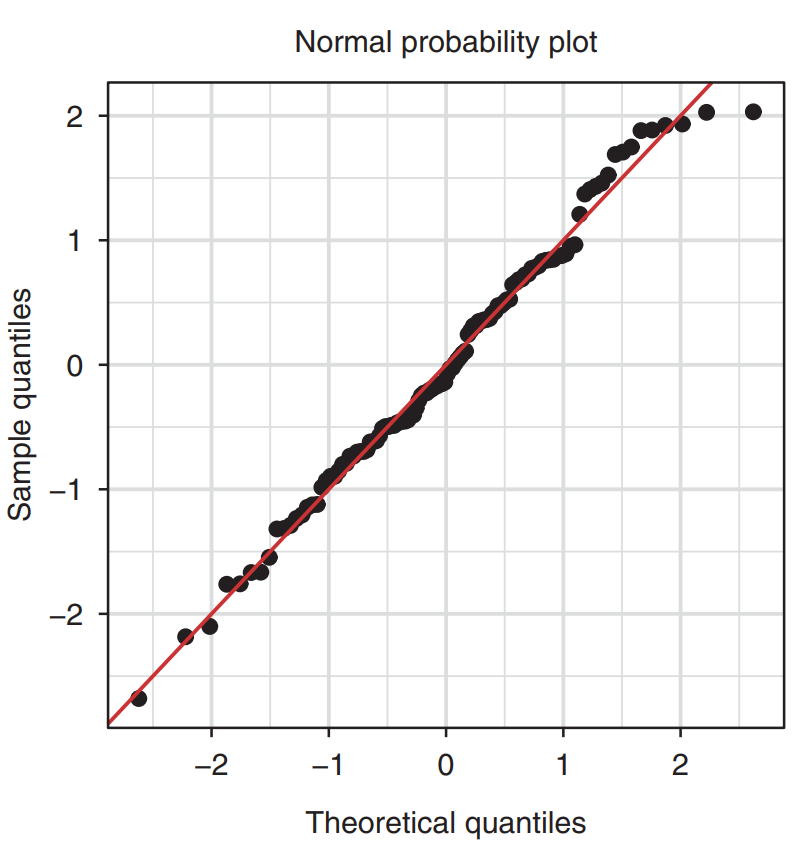
\includegraphics[scale=0.4]{gambar/plotregresilinear.png}
  \caption{Contoh plot untuk regresi linear (Rivera, 2020).}
  \label{fig:plotregresilinear}
\end{figure}

Regresi linier melayani tiga tujuan utama: menggambarkan fenomena data, kontrol, dan prediksi. Pertama, analisis regresi memungkinkan deskripsi fenomena data dengan membuat model hubungan numerik. Model ini membantu untuk memahami pola dan hubungan yang mendasari data yang sedang dipelajari.Kedua, regresi dapat digunakan untuk tujuan kontrol. Dengan menggunakan model regresi yang diperoleh, dimungkinkan untuk mengontrol atau memanipulasi variabel independen untuk melihat pengaruhnya terhadap variabel dependen. Hal ini memungkinkan untuk mempelajari hubungan sebab-akibat dan menentukan pengaruh variabel tertentu pada hasil yang diinginkan.Terakhir, analisis regresi memfasilitasi prediksi. Model regresi dapat digunakan untuk membuat prediksi terhadap variabel dependen. Namun, penting untuk dicatat bahwa prediksi terbatas pada kisaran variabel independen yang digunakan dalam membangun model regresi. Misalnya, jika model regresi dibangun menggunakan data variabel independen yang berkisar antara 5 hingga 25, prediksi hanya dapat dilakukan dalam rentang tersebut. Konsep ini dikenal sebagai interpolasi, di mana prediksi dibuat untuk nilai-nilai dalam rentang variabel independen yang diamati (Sulardi et al., 2017).

Dalam regresi linier, variabel bebas X dapat didasarkan pada data pengamatan atau data eksperimen/tetap. Data observasi mengacu pada data yang tidak ditentukan sebelumnya oleh peneliti dan diperoleh melalui observasi di lapangan. Di sisi lain, data eksperimen atau tetap mengacu pada data yang telah dikontrol atau ditentukan oleh peneliti sebelumnya, biasanya melalui eksperimen laboratorium.Perbedaan utama antara kedua jenis data ini terletak pada tingkat kontrol dan kemampuan untuk membangun hubungan sebab akibat. Saat menggunakan data tetap, peneliti memiliki nilai yang telah ditentukan sebelumnya untuk variabel independen X yang ingin mereka selidiki. Ini memungkinkan pengaturan yang lebih terkontrol dan memungkinkan peneliti untuk membangun hubungan kausal yang lebih kuat antara variabel X dan variabel dependen Y. Sebaliknya, data observasi tidak serta merta membangun hubungan sebab akibat. Variabel X dalam data observasi dapat diamati dengan berbagai cara, tergantung pada situasi nyata di lapangan. Data observasi sering dikumpulkan melalui kuesioner atau survei, dan peneliti kurang memiliki kendali atas variabel yang diteliti.


\subsection{Regresi Polinomial}
\label{subsec:regresipolinomial}

Regresi polinomial adalah teknik statistik yang memungkinkan pemodelan hubungan antara beberapa variabel independen (X dan Y) dan variabel dependen (Z) melalui hubungan non-linear (Shanock et al., 2010). Prosesnya melibatkan analisis hierarki persamaan polinomial, dengan memasukkan suku-suku orde tinggi sampai varians yang dijelaskan oleh persamaan orde tinggi berikutnya tidak lagi signifikan secara statistik. Awalnya, skor komponen untuk X dan Y (direpresentasikan sebagai X1 dan Y1) digunakan untuk menguji hubungan liniernya dengan Z pada tahap pertama analisis. Pada tahap kedua, suku orde tinggi (X2 dan Y2) dimasukkan ke dalam persamaan bersama dengan suku hasil kali (XY) untuk menilai keberadaan hubungan lengkung (khususnya, kuadrat). Selain itu, regresi polinomial, dikombinasikan dengan metodologi permukaan respons, menawarkan kerangka kerja untuk menguji dan menginterpretasikan fitur permukaan yang sesuai dengan persamaan regresi kuadrat polinomial. Teknik-teknik ini umumnya digunakan dalam penelitian organisasi, baik di tingkat mikro maupun makro, untuk menguji kesesuaian dan/atau perbedaan antar variabel (Shanock et al., 2010).

Metodologi ini memungkinkan peneliti untuk mengeksplorasi bagaimana kombinasi dua variabel prediktor dikaitkan dengan variabel hasil. Mereka telah menemukan aplikasi yang luas dalam penelitian umpan balik multi-sumber (Shanock et al., 2010). Kombinasi dari teknik-teknik ini menawarkan alat statistik yang memungkinkan pemeriksaan mendalam tentang hubungan tripartit. Dengan menyelidiki variabel dalam ruang tiga dimensi, ini memberikan wawasan tentang hubungan antara kombinasi dua variabel prediktor dan variabel hasil (Shanock et al., 2010).

Regresi polinomial dan metodologi permukaan respons dapat diterapkan dalam skenario di mana penyelidikan berfokus pada bagaimana kombinasi dua variabel prediktor berhubungan dengan suatu hasil. Namun, asumsi tertentu harus dipenuhi untuk menggunakan teknik ini secara efektif. Pertama, variabel prediktor harus sepadan, mewakili domain konseptual yang sama dan memungkinkan interpretasi yang berarti dari hubungannya dengan variabel dependen. Kedua, jika skala variabel prediktor berbeda, mereka harus diubah atau distandarisasi menjadi metrik umum. Ketiga, asumsi standar yang terkait dengan regresi berganda perlu dipenuhi (Sedera et al., 2019). Regresi polinomial dapat digunakan sebagai alternatif regresi moderat untuk memeriksa hubungan antara kombinasi variabel, menawarkan kekuatan penjelas yang lebih besar dan pandangan bernuansa dalam ruang tiga dimensi. Selanjutnya, teknik ini cocok ketika asumsi teoretis yang mendasari menunjukkan hubungan non-linear antara variabel independen dan dependen. Setelah asumsi terpenuhi, regresi polinomial dilakukan untuk menyelesaikan persamaan polinomial dan mendapatkan output. Keluaran ini kemudian dapat diproyeksikan ke permukaan respons tiga dimensi. Panduan langkah demi langkah terperinci untuk melakukan regresi polinomial dan membuat permukaan respons menggunakan keluaran polinomial disediakan oleh Shanock et al. (Shanock et al., 2010).

Pada Gambar 1, Panel A menampilkan sumbu X, Y, dan Z bersama dengan garis kongruensi dan inkongruensi. Di sisi lain, Panel B menunjukkan grafik permukaan respons sampel yang menampilkan dua variabel prediktor (X dan Y) dan satu variabel dependen (Z) (Sedera et al., 2019).

\begin{figure}[H]
  \centering
  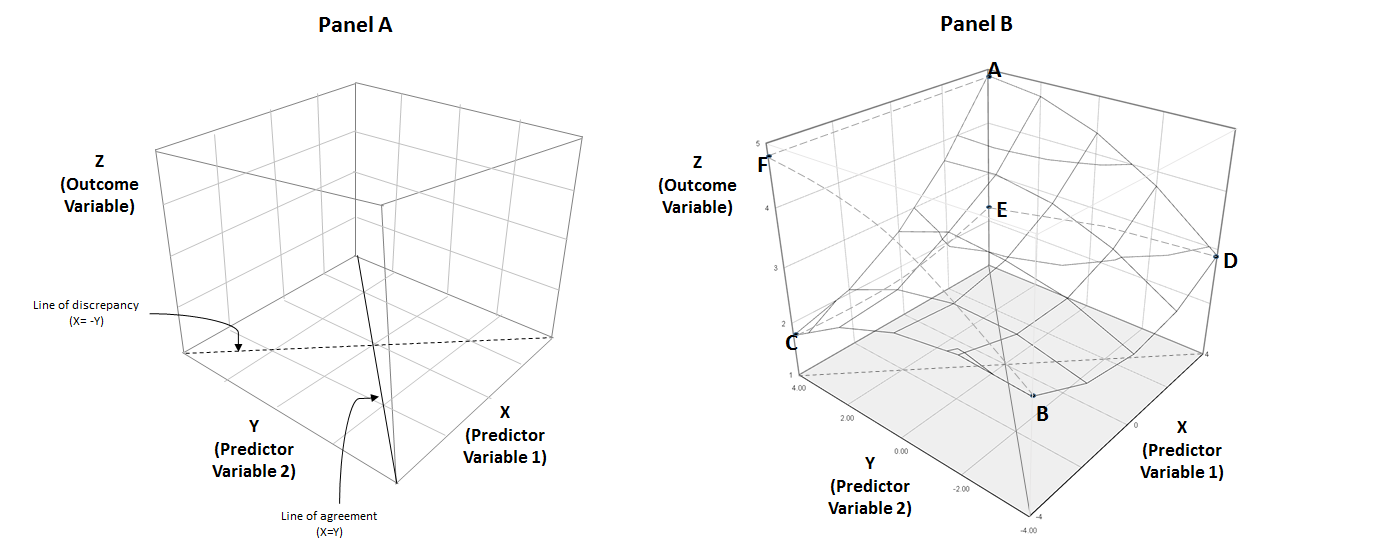
\includegraphics[scale=1]{gambar/plotregresipoli.png}
  \caption{Contoh plot untuk regresi polinomial pada 3D (Sedera et al., 2019).}
  \label{fig:plotregresipoli}
\end{figure}

\section{\emph{Machine Learning}}
\label{sec:machinelearning}

\emph{Machine Learning} (ML) adalah cabang ilmu komputasi yang muncul dari studi klasifikasi data dan prinsip-prinsip \emph{Artificial Intelligence} (AI). Bidang ini melibatkan pelatihan komputer untuk belajar secara otomatis dari input data, tanpa perlu pemrograman eksplisit. Konsep pembelajaran dalam pembelajaran mesin menarik kesejajaran dari pembelajaran manusia dan hewan. Faktanya, banyak teknik pembelajaran mesin terinspirasi oleh model komputasi berdasarkan prinsip pembelajaran hewan dan manusia. Misalnya, pembiasaan adalah perilaku kognitif mendasar yang diamati pada hewan, di mana mereka secara bertahap berhenti merespons rangsangan berulang. Anjing, misalnya, berfungsi sebagai contoh utama pembelajaran hewan, karena mereka dapat menjalani pelatihan substansial untuk melakukan berbagai aktivitas seperti berguling, duduk, dan mengambil objek (Datta \& Davim, 2022).

\begin{figure}[H]
  \centering
  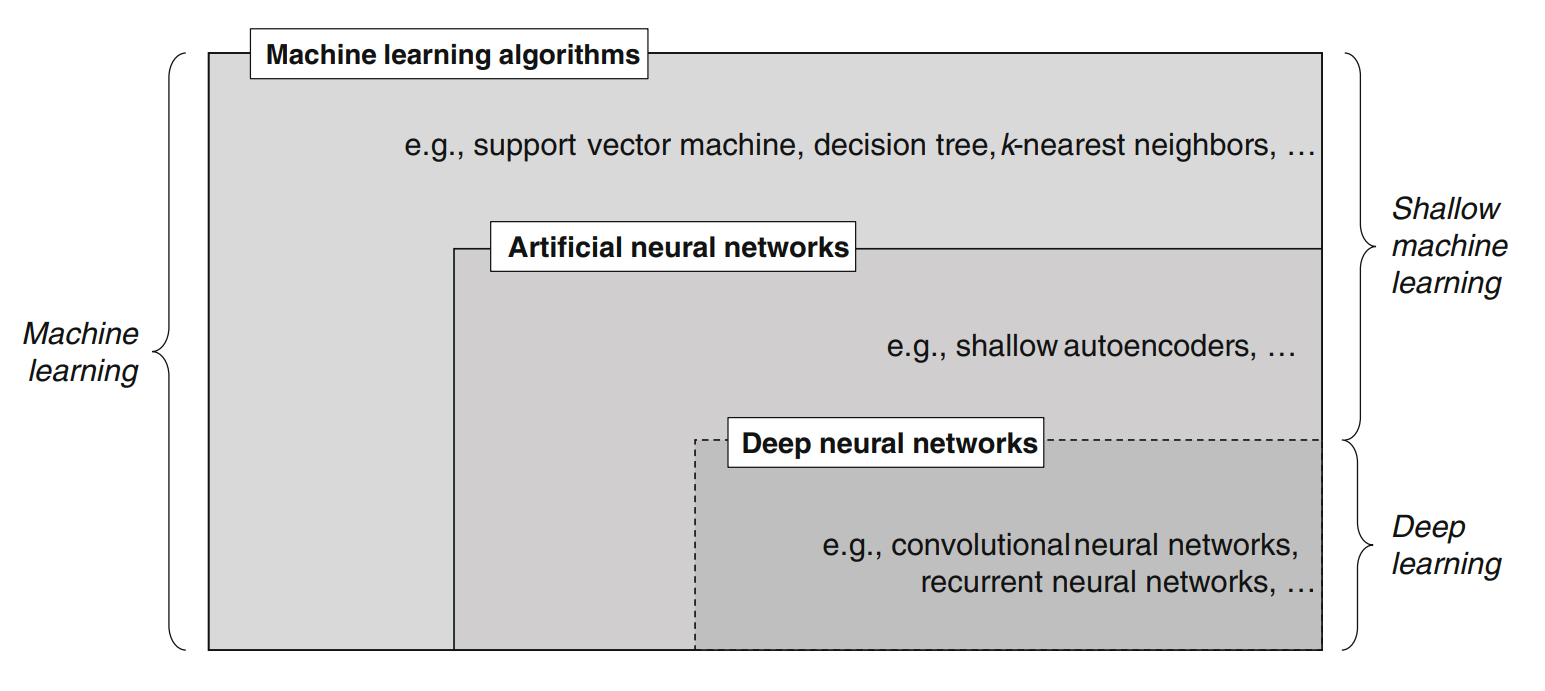
\includegraphics[scale=0.3]{gambar/machinelearning.png}
  \caption{Diagram Venn konsep dan kelas \emph{machine learning} (Janiesch et al., 2021).}
  \label{fig:machinelearningdiagram}
\end{figure}

Pembelajaran mesin menemukan aplikasi praktis dalam berbagai aspek kehidupan kita sehari-hari di era modern. Misalnya, asisten pribadi virtual, seperti Siri atau Alexa, menggunakan teknik pembelajaran mesin untuk memahami dan merespons perintah pengguna. Sistem navigasi GPS memanfaatkan pembelajaran mesin untuk memprediksi kondisi lalu lintas dan menyarankan rute yang optimal. Sistem pengawasan bertenaga AI dapat menganalisis umpan dari beberapa kamera untuk mendeteksi potensi kejahatan atau perilaku yang tidak biasa. Platform media sosial memanfaatkan pembelajaran mesin untuk tugas-tugas seperti pengenalan wajah dan kurasi umpan berita yang dipersonalisasi. Mesin pencari terus menyempurnakan hasil mereka menggunakan algoritma pembelajaran mesin. Filter spam email belajar dari email spam berlabel sebelumnya untuk mengidentifikasi dan memblokir pesan yang tidak diinginkan. Ini hanyalah beberapa contoh yang menunjukkan penggunaan luas pembelajaran mesin dalam aplikasi praktis. Memasukkan pengetahuan sebelumnya ke dalam proses pembelajaran dapat secara signifikan meningkatkan keefektifannya. Pembelajaran mesin juga terkait erat dengan statistik komputasi, memungkinkan pemodelan prediktif. Pentingnya pembelajaran mesin terletak pada pemahaman bagaimana hewan dan manusia belajar, serta dalam berbagai tujuan praktisnya (Datta \& Davim, 2022).

\subsection{\emph{Supervised Learning}}
\label{subsec:supervisedlearning}

Pembelajaran yang diawasi melibatkan penggunaan kumpulan data pelatihan yang berisi contoh dengan data input dan nilai target berlabel. Misalnya, memprediksi jumlah pengguna aktif pada platform pasar di bulan mendatang dapat dianggap sebagai tugas pembelajaran yang diawasi. Dalam hal ini, fitur input, seperti jumlah produk yang terjual atau review pengguna yang positif, digunakan untuk memprediksi variabel target atau output (sering dinotasikan sebagai variabel "y"). Dataset pelatihan digunakan untuk menyesuaikan parameter model pembelajaran mesin. Setelah model berhasil dilatih, model tersebut dapat diterapkan untuk memprediksi variabel target untuk titik data baru atau yang tidak terlihat berdasarkan fitur inputnya. Pembelajaran yang diawasi dapat dikategorikan lebih lanjut ke dalam masalah regresi, di mana nilai numerik diprediksi (mis., Jumlah pengguna), dan masalah klasifikasi, di mana hasil prediksi mewakili label kelas kategori, seperti "penonton" atau "pembeli" (Janiesch et al., 2021).

\subsection{\emph{Unsupervised Learning}}
\label{subsec:unsupervisedlearning}

Pembelajaran tanpa pengawasan terjadi ketika sistem pembelajaran ditugaskan untuk mengidentifikasi pola dalam data tanpa label atau spesifikasi yang telah ditentukan sebelumnya. Dalam pembelajaran tanpa pengawasan, data pelatihan hanya terdiri dari variabel (dilambangkan sebagai "x"), yang bertujuan untuk menemukan informasi struktural yang bermakna. Ini dapat melibatkan pendeteksian kelompok elemen yang memiliki sifat umum, yang dikenal sebagai pengelompokan, atau pengurangan dimensi data dengan memproyeksikannya dari ruang dimensi yang lebih tinggi ke ruang dimensi yang lebih rendah, yang dikenal sebagai pengurangan dimensi. Dalam konteks pasar elektronik, contoh menonjol dari pembelajaran tanpa pengawasan adalah penerapan teknik pengelompokan untuk mengelompokkan pelanggan atau pasar ke dalam segmen-segmen. Ini memungkinkan komunikasi yang lebih bertarget dan spesifik yang disesuaikan dengan kelompok pelanggan yang berbeda (Janiesch et al., 2021).

\subsection{\emph{Semi Supervised Learning}}
\label{subsec:semiisupervisedlearning}

Pembelajaran semi-diawasi adalah pendekatan hybrid yang menggabungkan metode pembelajaran yang diawasi dan tidak diawasi, dengan fokus pada penggunaan sampel berlabel dan tidak berlabel secara efektif selama proses pelatihan. Ini bertujuan untuk membangun hubungan antara sampel yang diprediksi dan tujuan pembelajaran berdasarkan hipotesis tertentu. Asumsi kehalusan menunjukkan bahwa sampel yang terletak berdekatan di wilayah kepadatan tinggi lebih cenderung memiliki label kelas yang sama. Asumsi cluster berpendapat bahwa sampel yang termasuk dalam cluster yang sama sangat mungkin untuk berbagi kelas yang sama. Terakhir, asumsi manifold mengusulkan bahwa sampel dalam lingkungan lokal kecil dalam manifold berdimensi rendah cenderung memiliki label kelas yang serupa (Wang et al., 2023).

\subsection{\emph{Reinforcement Learning}}
\label{subsec:reinforcementlearning}

Dalam sistem pembelajaran penguatan, pendekatannya berbeda dengan pemberian pasangan input-output. Sebaliknya, sistem dijelaskan oleh keadaan saat ini, tujuan yang ditentukan, serangkaian tindakan yang diizinkan, dan kendala lingkungan terkait untuk setiap hasil tindakan. Model pembelajaran mesin kemudian belajar dengan secara aktif terlibat dalam proses pencapaian tujuan melalui coba-coba, yang bertujuan untuk memaksimalkan hadiah. Pembelajaran penguatan telah menunjukkan pencapaian yang signifikan dalam lingkungan yang terkendali seperti permainan dan juga berlaku untuk sistem multi-agen seperti pasar elektronik (Janiesch et al., 2021).

\section{\emph{Deep Learning}}
\label{sec:deeplearning}

\emph{Deep learning} adalah cabang \emph{machine learning} yang melibatkan penggunaan beberapa lapisan pemrosesan informasi nonlinier untuk melakukan tugas-tugas seperti ekstraksi fitur, pengenalan pola, dan klasifikasi (Deng dan Yu, 2014). Menurut Goodfellow, dkk. (2016) dalam \emph{deep learning}, konsep kompleks dipelajari dengan menggabungkan konsep yang lebih sederhana secara hierarkis. Struktur hierarkis ini memungkinkan komputer mempelajari dan memahami pola dan hubungan yang rumit di dalam data. Istilah "dalam" mengacu pada beberapa lapisan dalam jaringan, membentuk grafik yang dalam saat divisualisasikan, oleh karena itu dinamakan "pembelajaran mendalam". \emph{Deep learning} telah terbukti sangat efektif di berbagai bidang, termasuk visi komputer, pemrosesan bahasa alami, dan pengenalan suara.

\emph{Deep learning} dicirikan oleh arsitekturnya yang terdiri dari beberapa lapisan, umumnya dikenal sebagai \emph{hidden layer}, yang ditumpuk bersama. Setiap lapisan dalam arsitektur ini berfungsi sebagai algoritma atau metode yang mengambil input dan menghasilkan output melalui serangkaian komputasi. Salah satu metode \emph{deep learning} yang menonjol adalah \emph{Convolutional Neural Network} (CNN). CNN dirancang khusus untuk memproses input gambar. Gambar input melewati lapisan konvolusional, di mana diproses menggunakan filter yang mengekstraksi pola dari berbagai bagian gambar. Ekstraksi pola hierarkis dari gambar ini membantu dalam proses klasifikasi. CNN telah menunjukkan keberhasilan luar biasa dalam berbagai tugas terkait gambar seperti pengenalan objek, klasifikasi gambar, dan segmentasi gambar (Danukusumo, 2017).

\begin{figure}[H]
  \centering
  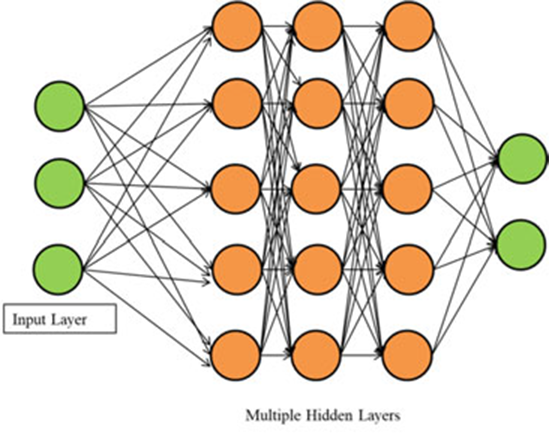
\includegraphics[scale=1]{gambar/arsitekturdlnn.png}
  \caption{Arsitektur \emph{deep learning} (Janiesch et al., 2021)}
  \label{fig:arsidl}
\end{figure}


Di bidang pengenalan citra, \emph{Convolutional Neural Network} (CNN) saat ini merupakan metode \emph{deep learning} yang paling berdampak (Nugroho et al., 2020). CNN sangat berhasil dalam lingkup ini karena mencoba meniru sistem pengenalan gambar dari korteks visual manusia, memungkinkannya memproses informasi gambar secara efektif. Namun, seperti metode pembelajaran mendalam lainnya, CNN memiliki kekurangan, yaitu proses pelatihan yang lama. Untungnya, kemajuan teknologi perangkat keras, seperti penggunaan \emph{General Purpose Graphical Processing Unit} (GPGPU), telah membantu mengatasi tantangan ini.

CNN dirancang dengan fokus khusus pada tugas yang terkait dengan pengenalan dan klasifikasi gambar. Arsitektur dan strukturnya disesuaikan untuk memproses dan menganalisis data gambar secara efisien. Ini terdiri dari beberapa lapisan yang mengekstrak informasi yang relevan dari gambar dan membuat prediksi tentang klasifikasinya melalui skor klasifikasi. Lapisan di CNN, seperti lapisan konvolusional dan lapisan penyatuan, memainkan peran penting dalam menangkap fitur dan pola hierarki dalam gambar, memungkinkan pengenalan dan klasifikasi yang akurat. Secara keseluruhan, kemampuan CNN untuk mempelajari dan menginterpretasikan data visual yang kompleks menjadikannya metode terdepan dalam bidang pengenalan gambar.

\subsection{\emph{Neural Network}}
\label{subsec:cnn}

Artificial Neural Networks (ANNs) adalah sistem komputasi yang mengambil inspirasi dari Biological Neural Networks (BNNs). Mereka menawarkan solusi yang efektif untuk berbagai tugas, seperti klasifikasi, prediksi, pemfilteran, pengoptimalan, pengenalan pola, dan perkiraan fungsi. Sementara sistem saraf biologis sangat rumit, JST bertujuan untuk menyederhanakan dan abstrak kompleksitas ini, berfokus pada aspek-aspek penting yang relevan dengan pemrosesan informasi. Jaringan saraf awalnya diperkenalkan oleh McCulloch dan Pitts pada tahun 1990 ketika mereka berusaha memodelkan pemrosesan informasi secara matematis dalam sistem biologis. Jaringan ini terdiri dari simpul yang saling berhubungan, menyerupai neuron yang ditemukan di otak organisme hidup. Setiap node menghitung jumlah bobot inputnya, memprosesnya di dalam lapisan tersembunyi, dan menghasilkan output dengan menerapkan fungsi aktivasi ke nilai bobot (Thakur et al., 2021).

\begin{figure}[H]
  \centering
  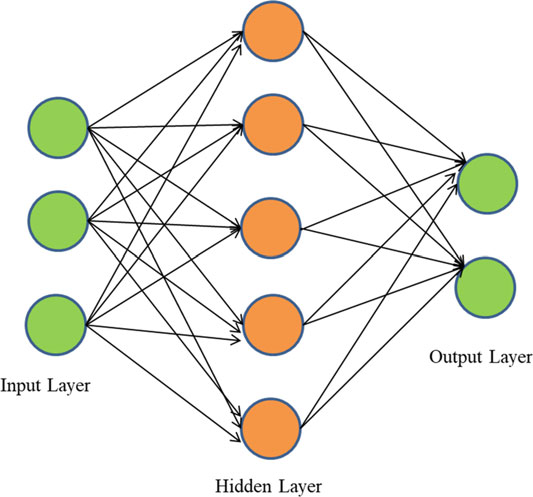
\includegraphics[scale=1]{gambar/arsitekturann.png}
  \caption{Arsitektur \emph{neural network} (Janiesch et al., 2021)}
  \label{fig:arsiann}
\end{figure}

Neural network telah berevolusi dari arsitektur sederhana menjadi struktur yang semakin kompleks. Awalnya, jaringan saraf memiliki arsitektur yang sangat dasar yang hanya terdiri dari lapisan masukan dan keluaran, sering disebut sebagai jaringan lapisan tunggal. Namun, dengan memasukkan lapisan tersembunyi ke dalam jaringan saraf satu lapis, itu menjadi jaringan saraf multi-lapisan. Akibatnya, jaringan saraf multi-layer terdiri dari lapisan input, lapisan tersembunyi, dan lapisan output, seperti yang diilustrasikan pada gambar yang diberikan (Thakur et al., 2021).

\section{\emph{Convolutional Neural Network}}
\label{sec:cnn}

\emph{Convolutional Neural Network} (CNN) adalah jenis jaringan saraf khusus yang biasa digunakan dalam tugas pemrosesan gambar untuk mendeteksi dan mengenali objek di dalam gambar (Mehindra, 2020). CNN dirancang untuk memproses data yang diatur dalam struktur seperti kisi, seperti gambar. Mereka dapat dianggap sebagai kombinasi jaringan syaraf tiruan dan metode pembelajaran mendalam (Fonda, 2020). Arsitektur CNN tipikal terdiri dari satu atau lebih lapisan konvolusional, yang melakukan konvolusi pada data input, diikuti oleh lapisan downsampling, sering disebut sebagai lapisan penyatuan. Lapisan-lapisan ini membantu mengurangi dimensi spasial data sambil mempertahankan fitur-fitur penting. Terakhir, satu atau lebih lapisan yang terhubung sepenuhnya digabungkan, mirip dengan jaringan saraf tradisional, untuk memproses fitur yang diekstraksi dan membuat prediksi. Dengan menggunakan lapisan konvolusional, CNN efektif dalam menangkap ketergantungan spasial dan lokal dalam gambar, memungkinkan mereka untuk mempelajari representasi dan pola yang bermakna. Ini membuat CNN sangat cocok untuk tugas-tugas seperti klasifikasi gambar, deteksi objek, dan segmentasi gambar.

Arsitektur CNN dapat dibagi menjadi dua bagian utama, yaitu \emph{Fully-Connected Layer} dan \emph{Multi-Layer Perceptron} (MLP). CNN terdiri dari beberapa lapisan yang melakukan operasi tertentu. Mengikuti arsitektur LeNet5, terdapat empat layer utama dalam sebuah CNN berupa \emph{Convolution Layer, Pooling Layer, Subsampling Layer,} dan \emph{Fully Connected Layer} (Eka Putra, 2016). 

\begin{figure}[H]
  \centering
  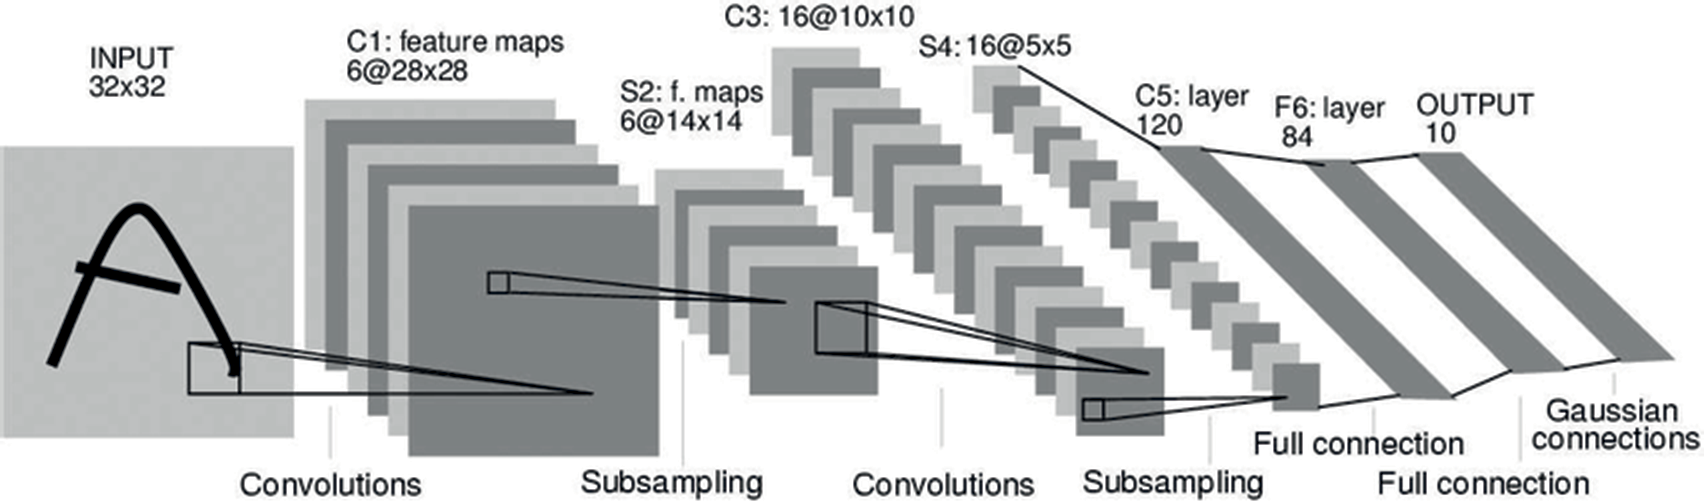
\includegraphics[scale=0.8]{gambar/arsitekturcnn.png}
  \caption{Arsitektur \emph{convolutional neural network} oleh LeNet-5 (LeCun et al., 1998)}
  \label{fig:arsicnn}
\end{figure}

\emph{Convolution Layer} menerapkan operasi konvolusi untuk mengekstraksi fitur dari data masukan. Ini menggunakan filter untuk mendeteksi berbagai pola dan struktur dalam data. \emph{Pooling layer} mengurangi dimensi spasial dari fitur yang diekstraksi sambil mempertahankan karakteristik pentingnya. Ini membantu mengurangi kompleksitas komputasi dan membuat jaringan lebih kuat terhadap variasi dalam input data. \emph{Subsampling layer} selanjutnya mengurangi dimensi data melalui \emph{downsampling}, menangkap informasi yang paling signifikan. Terakhir, \emph{Fully-Connected Layer}, yang serupa dengan \emph{Multi-Layer Perceptron} (MLP), menerima fitur yang diproses dan melakukan tugas klasifikasi atau regresi. Ini menghubungkan semua neuron dari lapisan sebelumnya ke lapisan keluaran, memungkinkan jaringan membuat prediksi berdasarkan fitur yang dipelajari. Lapisan-lapisan ini bekerja sama dalam CNN untuk mengekstraksi dan mengubah data input menjadi representasi yang bermakna, yang pada akhirnya memungkinkan jaringan untuk melakukan tugas-tugas seperti pengenalan gambar dan klasifikasi secara efektif.

Pada CNN, data yang diproses oleh jaringan berupa data dua dimensi. Ini memerlukan adaptasi khusus dalam hal operasi linier dan bobot parameter di CNN dibandingkan dengan jaringan saraf tradisional. CNN menggunakan operasi konvolusi untuk operasi linier, dan bobot direpresentasikan dalam empat dimensi sebagai sekumpulan kernel konvolusi. Karena sifat yang melekat pada proses konvolusi, CNN cocok untuk menganalisis data dengan struktur dua dimensi, seperti gambar dan suara.

Sebagai contoh adalah data yang diproses CNN berupa gambar dua dimensi. Istilah "konvolusi" mengacu pada operasi aljabar linier di mana matriks filter dikalikan dengan matriks gambar yang sedang diproses. Operasi ini dikenal sebagai lapisan konvolusi, yang merupakan salah satu dari beberapa jenis lapisan yang dapat hadir dalam CNN. Lapisan konvolusi sangat penting dan banyak digunakan dalam arsitektur CNN. Lapisan lain yang umum digunakan adalah \emph{Pooling layer}, yang mengagregasi informasi dengan mengambil nilai maksimum atau rata-rata dari wilayah piksel di dalam gambar. Setiap lapisan masukan dalam CNN memiliki volume berbeda yang ditandai dengan kedalaman, tinggi, dan lebarnya. Nilai yang didapat pada setiap layer dipengaruhi oleh hasil proses penyaringan dari layer sebelumnya, serta jumlah filter yang digunakan. Model jaringan ini telah menunjukkan kemanjuran yang luar biasa dalam menangani tugas klasifikasi gambar.

\subsection{\emph{Convolutional Layer}}
\label{subsec:cnn}

Operasi konvolusi adalah komponen fundamental dari jaringan saraf convolutional (CNN). Lapisan convolutional dari CNN terdiri dari satu set filter yang dapat dipelajari, juga dikenal sebagai kernel. Setiap filter berukuran kecil, biasanya 3x3, 5x5, atau 7x7, dan menjangkau seluruh kedalaman volume input. Kedalaman filter sesuai dengan jumlah saluran dalam masukan, dengan gambar skala abu-abu memiliki kedalaman 1 dan gambar berwarna memiliki 3 saluran (RGB) (Bezdan et al., 2019). 

Selama proses propagasi maju dalam jaringan saraf convolutional, setiap filter melakukan konvolusi pada volume input dengan menghitung perkalian titik antara entri filter dan nilai input yang sesuai di setiap posisi. Operasi ini diikuti dengan menerapkan fungsi aktivasi nonlinier, seperti sigmoid, tanh, atau ReLU, ke hasilnya, yang menghasilkan peta fitur. Peta fitur mewakili respons filter pada posisi spasial yang berbeda. Peta aktivasi ini ditumpuk sepanjang dimensi kedalaman untuk membentuk volume keluaran. Karakteristik volume output ditentukan oleh tiga hyperparameter: depth, stride, dan padding (Bezdan et al., 2019).

Kedalaman volume keluaran sesuai dengan jumlah filter yang digunakan dalam operasi konvolusi. Setiap filter mempelajari aspek input yang berbeda, seperti tepi, blob, atau warna. Langkahnya menentukan jumlah langkah filter bergerak melintasi input. Langkah 1 menggerakkan filter satu piksel pada satu waktu, sedangkan langkah 2 membuat filter melompati 2 piksel sekaligus, menghasilkan volume output yang lebih kecil secara spasial. Padding digunakan untuk mengontrol ukuran output. Ini melibatkan penambahan nol di sekitar batas volume input untuk menyimpan informasi dan menghindari pengurangan ukuran output. Ada dua pilihan umum: valid convolution, yang berarti tidak ada padding, dan same convolution, di mana ukuran output tetap sama dengan ukuran input (Bezdan et al., 2019).

\subsection{\emph{Pooling Layer}}
\label{subsec:cnn}

Pooling layer di CNN sering digunakan setelah convolutional layer untuk mengurangi dimensi peta fitur. Operasi ini juga dikenal sebagai subsampling atau downsampling. Hyperparameters dari pooling layer mencakup ukuran dan langkah filter. Lapisan penyatuan yang paling umum digunakan memiliki ukuran filter 2 dan langkah 2. Ada dua jenis utama penyatuan lapisan: penyatuan maks dan penyatuan rata-rata. Max pooling memilih nilai maksimum dalam setiap wilayah, sedangkan average pooling menghitung nilai rata-rata. Max pooling lebih umum digunakan daripada pooling rata-rata. Penting untuk diperhatikan bahwa pooling layer tidak memiliki parameter yang dapat dipelajari. Tujuan max pooling adalah untuk menangkap fitur yang paling menonjol dengan memilih nilai terbesar (Bezdan et al., 2019).


\subsection{\emph{Fully Connected Layer}}
\label{subsec:cnn}

Setelah beberapa lapisan konvolusi dan penyatuan, CNN biasanya diakhiri dengan beberapa lapisan yang terhubung sepenuhnya. Output tensor dari lapisan sebelumnya diratakan menjadi vektor, dan kemudian ditambahkan lapisan jaringan saraf tambahan. Lapisan yang terhubung penuh ini biasanya diposisikan menjelang akhir arsitektur, seperti yang digambarkan pada Gambar 3. Untuk mencegah overfitting, teknik regularisasi dropout dapat digunakan pada lapisan yang terhubung penuh ini. Lapisan terhubung penuh terakhir dalam arsitektur terdiri dari jumlah neuron keluaran yang sama dengan jumlah kelas yang akan dikenali (Bezdan et al., 2019).

\section{Visi Komputer}
\label{sec:deteksigesturtubuh}

Visi komputer adalah bidang kecerdasan buatan yang bertujuan untuk meniru persepsi visual manusia dengan menggunakan algoritme dan sensor optik untuk mengekstrak informasi yang relevan dari objek. Tidak seperti metode tradisional yang melibatkan pemeriksaan laboratorium yang memakan waktu dan tenaga, visi komputer menawarkan pendekatan yang lebih efisien. Integrasi sistem pencahayaan dapat digunakan bersamaan dengan MediaPipe untuk meningkatkan proses akuisisi dan pemrosesan gambar. Proses analisis citra melibatkan beberapa langkah. Pertama, tahap pembentukan citra menangkap dan menyimpan citra suatu objek di dalam komputer. Selanjutnya, pra-pemrosesan gambar meningkatkan kualitas gambar untuk meningkatkan detail. Kemudian, segmentasi citra mengidentifikasi dan memisahkan citra objek dari latar belakang. Pada tahap pengukuran citra dilakukan pengukuran berbagai parameter penting. Akhirnya, interpretasi gambar melibatkan analisis dan pemahaman gambar yang diperoleh (Kotappa  et al., 2022).

\begin{figure}[H]
  \centering
  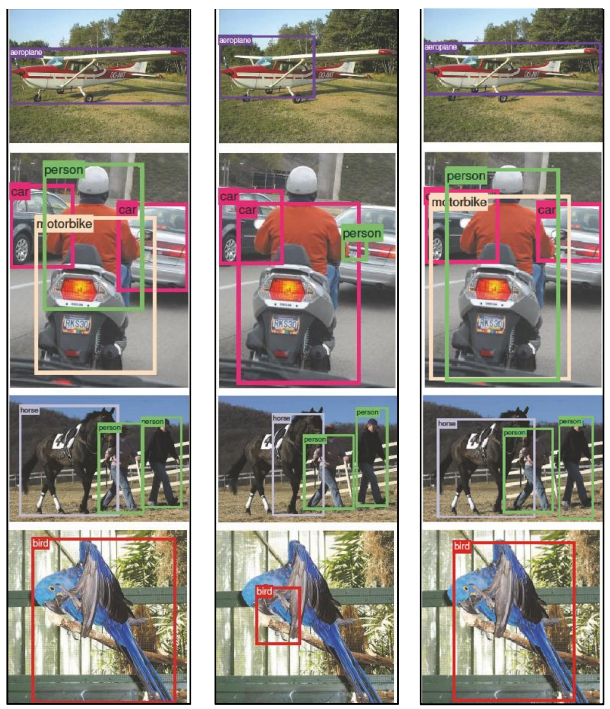
\includegraphics[scale=0.55]{gambar/computervision.png}
  \caption{Visi komputer pada deteksi objek (Shetty et al., 2022)}
  \label{fig:visikomdeteksi}
\end{figure}

Karena kemajuan terbaru dalam teknologi pemrosesan gambar, sekarang dimungkinkan untuk mengembangkan sistem yang dapat mengenali gambar digital. Bidang-bidang seperti matematika, aljabar linier, statistik, Soft Computing, dan ilmu saraf Komputasi telah memainkan peran penting dalam memajukan pemrosesan citra digital. Pengenalan pola, bagian dari visi komputer, berfokus pada identifikasi objek dengan meningkatkan kualitas gambar dan interpretasi melalui transformasi gambar. Ini melibatkan penggalian data dari gambar yang ditangkap sensor untuk membuat penilaian. Tujuan dari visi komputer adalah menciptakan mesin yang dapat "melihat". Kerangka umum dalam visi komputer mencakup pengambilan gambar, pemrosesan awal, ekstraksi fitur, deteksi/segmentasi, pemrosesan tingkat tinggi, dan pengambilan keputusan. Dalam visi komputer, ada kategori seperti analisis morfologi 3D dan pengoptimalan piksel. Optimalisasi piksel melibatkan karakterisasi morfologi piksel untuk pemrosesan gambar yang lebih baik dan pengenalan pola, sedangkan analisis morfologi 3D adalah teori standar dalam pemrosesan gambar komputer dan pengenalan pola (Kotappa  et al., 2022).

Kategori ini mencakup tugas-tugas yang terkait dengan pengambilan wilayah gambar tertentu, seperti kueri mesin telusur, penelusuran manusia, dan penelusuran gambar serupa. Metode segmentasi gambar, seperti pendekatan berbasis intensitas, berbasis warna, dan berbasis bentuk, biasanya digunakan untuk tujuan ini. Deteksi tepi dan segmentasi gambar sangat penting untuk pengenalan dan interpretasi objek dalam berbagai aplikasi visi komputer. Sementara gambar sampel kecil sering digunakan untuk mendemonstrasikan kinerja segmentasi dalam literatur analisis gambar, pengaturan parameter diperlukan untuk anotasi dalam database gambar berskala besar. Tekstur gradien dan pengelompokan tanpa pengawasan dalam ruang fitur digunakan untuk mencapai segmentasi. Segmentasi pelabelan yang akurat sangat penting untuk kinerja pelokalan dan pelokalan batas. Pendekatan pengelompokan dan segmentasi dapat digunakan untuk memperkirakan item dalam citra dengan menetapkan ambang batas pada metode pengelompokan fitur (Kotappa  et al., 2022).


\section{Treadmill}
\label{sec:deteksigesturtubuh}

Treadmill umumnya digunakan di bidang rehabilitasi untuk membantu pasien dengan gangguan gaya berjalan, seperti penyakit Parkinson, stroke, dan cedera tulang belakang, dalam pemulihan kemampuan berjalan mereka. Pelatihan treadmill menawarkan beberapa keuntungan dibandingkan dengan pelatihan di lapangan, antara lain bantuan yang dapat diakses, kebutuhan ruang yang lebih kecil, dan kemampuan untuk mengontrol kecepatan berjalan. Namun, penting untuk dicatat bahwa tujuan akhir rehabilitasi adalah agar pasien mendapatkan kembali kemampuannya untuk berjalan di tanah daripada hanya di atas treadmill. Oleh karena itu, sangat penting untuk memahami dampak berjalan treadmill pada tubuh manusia (Shi et al., 2019).

Bidang studi ini penting untuk tujuan pelatihan dan penelitian, dan ada temuan yang bertentangan dalam studi ilmiah mengenai topik ini. Beberapa penelitian telah menunjukkan bahwa berlari di atas treadmill dengan kecepatan sedang 3,3 hingga 4,8 m/s menghasilkan penurunan panjang langkah dan fase terbang, tetapi iramanya meningkat dibandingkan dengan berlari di tanah. Di sisi lain, penelitian lain telah menemukan kesamaan antara treadmill dan lari di atas tanah dalam hal faktor kinematik seperti sudut adduksi pinggul, rotasi pinggul internal / eksternal, eversi pergelangan kaki, dan rotasi panggul maksimum (Pakbaz et al., 2018).

Belakangan ini, penggunaan perangkat treadmill meningkat secara signifikan, menjadikannya pilihan populer di kalangan individu. Selain itu, treadmill telah mendapatkan popularitas sebagai alat penelitian di berbagai bidang investigasi karena keunggulan metodologinya, termasuk efisiensi ruang, reproduktifitas, dan kemampuan untuk mengontrol variabel seperti kondisi cuaca, kecepatan, dan kemiringan. Namun, penelitian yang dilakukan pada treadmill telah menghasilkan hasil yang bertentangan, yang mengarah ke pertanyaan tentang apakah kelelahan yang disebabkan oleh berlari di atas treadmill dibandingkan berlari di tanah memiliki efek yang berbeda pada distribusi tekanan plantar selama berlari (Pakbaz et al., 2018).

\begin{figure}[H]
  \centering
  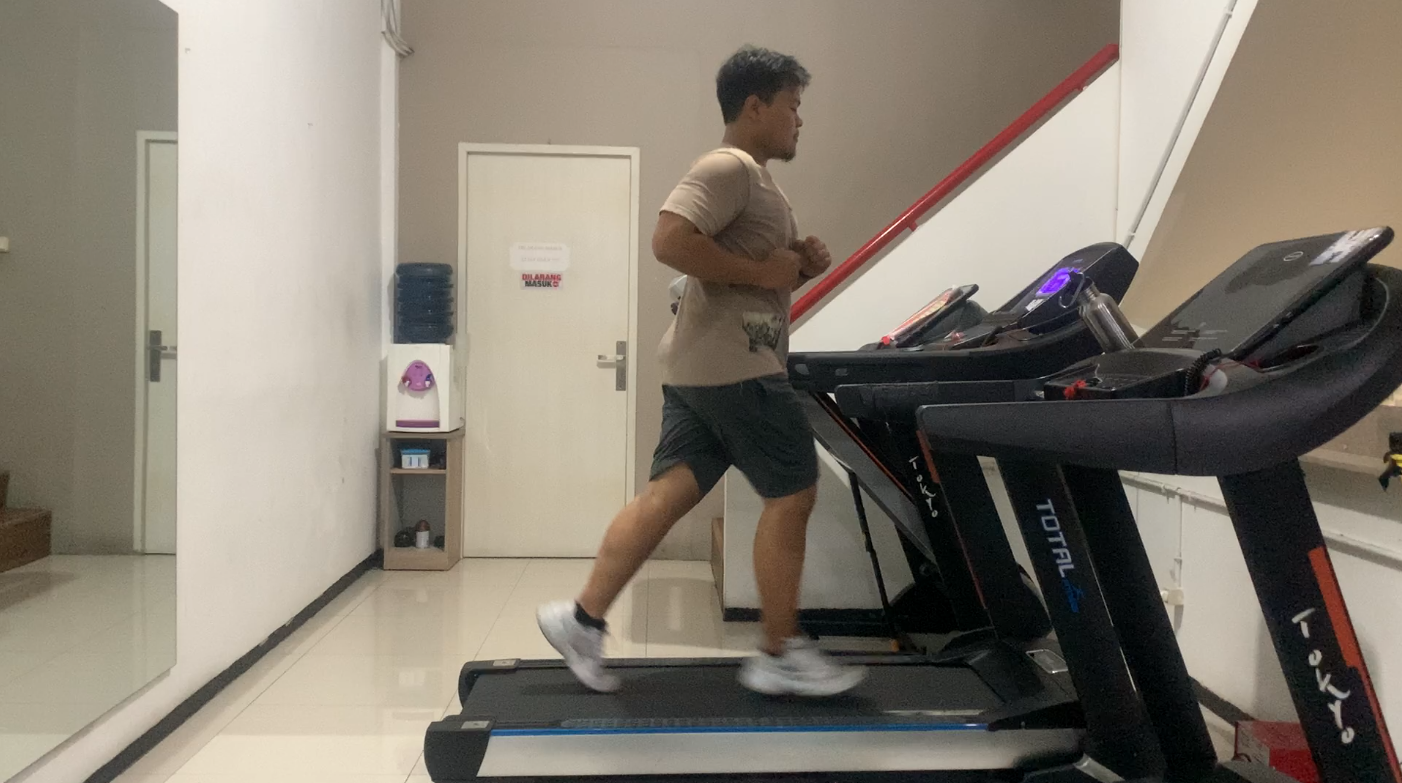
\includegraphics[scale=0.28]{gambar/treadmill.png}
  \caption{Olahraga pada treadmill.}
  \label{fig:treadmillrun}
\end{figure}

\section{\emph{Human Pose Estimation}}
\label{sec:deteksigesturtubuh}

Estimasi pose manusia bertujuan untuk menentukan posisi sendi manusia menggunakan berbagai sumber input seperti gambar, urutan gambar, gambar kedalaman, atau data kerangka yang diperoleh dari perangkat penangkap gerak. Tugas ini menantang karena faktor-faktor seperti penampilan manusia yang beragam, variasi siluet, kondisi pencahayaan yang menantang, dan latar belakang yang berantakan. Di masa lalu, estimasi pose bergantung pada teknik seperti deteksi bagian tubuh menggunakan struktur bergambar. Namun, dengan munculnya pembelajaran mendalam, ada dua pendekatan utama yang digunakan: metode holistik dan berbasis bagian (Shetty et al., 2022).

\begin{figure}[H]
  \centering
  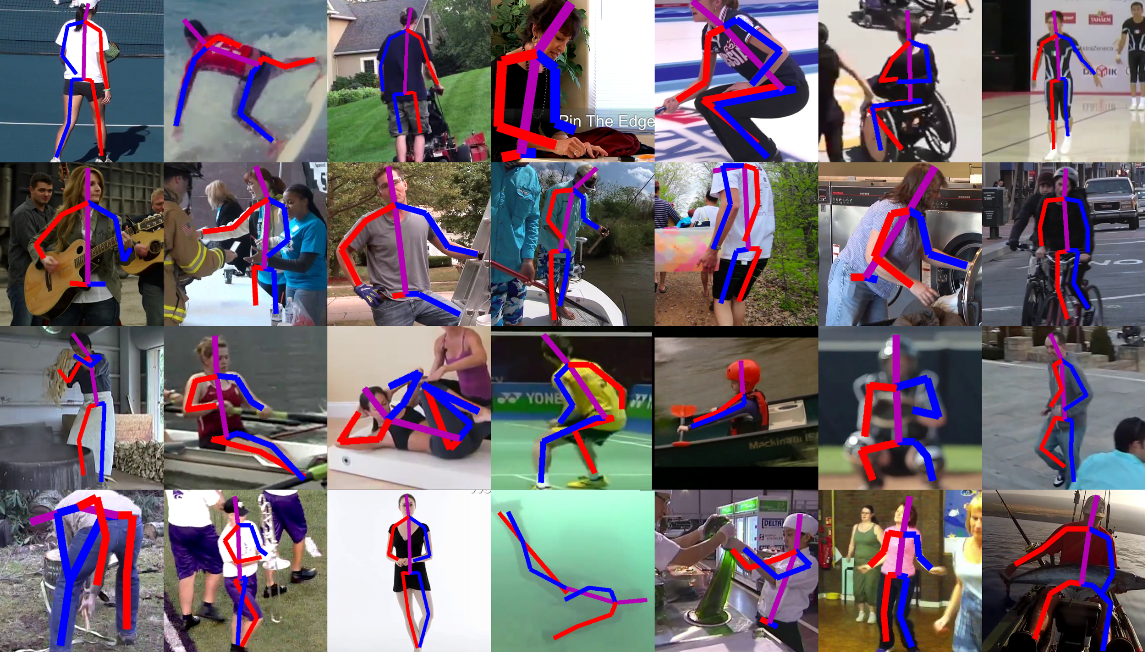
\includegraphics[scale=0.95]{gambar/humanpose.png}
  \caption{Contoh hasil \emph{human pose estimation} (Newell et al., 2016)}
  \label{fig:humanposeestimation}
\end{figure}

Metode holistik memproses gambar masukan secara global tanpa secara eksplisit memodelkan bagian tubuh individu dan hubungan spasialnya. Misalnya, DeepPose adalah model holistik yang memperlakukan estimasi pose manusia sebagai masalah regresi gabungan, tanpa secara eksplisit mendefinisikan model grafis atau pendeteksi bagian. Namun, pendekatan holistik mungkin berjuang dengan akurasi di wilayah presisi tinggi karena kesulitan untuk secara langsung meregresi vektor pose kompleks dari gambar (Shetty et al., 2022).

Di sisi lain, metode berbasis bagian secara eksplisit memodelkan bagian tubuh individu dan hubungan spasialnya. Metode ini menganalisis citra masukan dengan mempertimbangkan hubungan antara berbagai bagian tubuh manusia. Dengan memodelkan bagian-bagian secara eksplisit, pendekatan ini bertujuan untuk menangkap informasi yang lebih rinci tentang pose tersebut (Shetty et al., 2022).

Sebaliknya, metode berbasis bagian dalam estimasi pose manusia berfokus pada pendeteksian bagian tubuh individu secara terpisah dan kemudian menggunakan model grafis untuk memasukkan informasi spasial. Misalnya, dalam satu penelitian, alih-alih melatih jaringan pada seluruh gambar, penulis melatih jaringan saraf convolutional (CNN) menggunakan tambalan bagian lokal dan tambalan latar belakang untuk mempelajari probabilitas bersyarat dari kehadiran bagian dan hubungan spasial. Pendekatan lain melibatkan pelatihan beberapa CNN yang lebih kecil untuk klasifikasi bagian tubuh biner independen, diikuti oleh model spasial lemah tingkat tinggi untuk menghilangkan outlier dan memastikan konsistensi pose global. Selanjutnya,  multi-resolusi CNN dikembangkan untuk memperkirakan kemungkinan setiap bagian tubuh menggunakan peta panas, dan model grafis implisit diterapkan untuk menegakkan konsistensi sendi (Shetty et al., 2022).

\section{Mediapipe}
\label{sec:mediapipe}

MediaPipe adalah kerangka kerja yang dirancang untuk membuat jalur pipa untuk melakukan inferensi pada berbagai jenis data sensorik. Dengan menggunakan MediaPipe, dimungkinkan untuk membuat pipa yang terdiri dari komponen modular, termasuk inferensi model, algoritme pemrosesan media, dan transformasi data. Framework ini memungkinkan input data sensorik seperti audio dan video stream ke dalam pipeline, dan menghasilkan deskripsi yang dirasakan seperti lokalisasi objek dan face landmark stream sebagai outputnya (Lugaresi et al., 2019).

\begin{figure}[H]
  \centering
  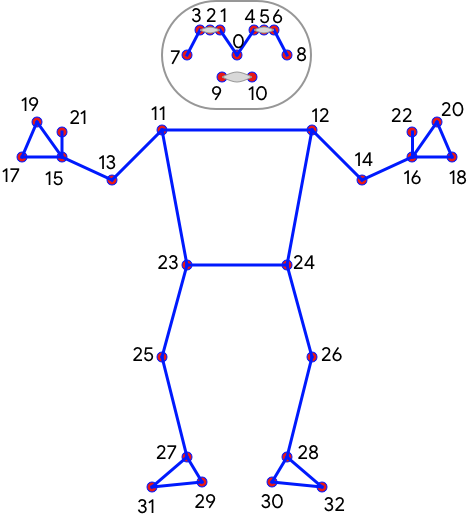
\includegraphics[scale=1.3]{gambar/mediapipeb2.png}
  \caption{Mediapipe \emph{keypoints} untuk estimasi pose (Bazarevsky et al., 2020).}
  \label{fig:mediapipe}
\end{figure}

MediaPipe adalah platform yang melayani praktisi pembelajaran mesin, termasuk peneliti, mahasiswa, dan pengembang perangkat lunak. Tujuannya adalah untuk membantu pengembangan aplikasi ML yang siap produksi, mendukung publikasi kode penelitian, dan memungkinkan pembuatan prototipe teknologi. Kasus penggunaan utama untuk MediaPipe adalah pembuatan pipeline persepsi yang cepat dan efisien dengan memanfaatkan model inferensi dan komponen yang dapat digunakan kembali. Selain itu, MediaPipe menyederhanakan penerapan teknologi persepsi dalam demonstrasi dan aplikasi di berbagai platform perangkat keras. Platform ini juga memfasilitasi peningkatan iteratif pada alur persepsi melalui bahasa konfigurasi dan alat evaluasinya yang komprehensif (Lugaresi et al., 2019).

\section{Metode Pengujian}
\label{sec:deteksigesturtubuh}

Pada metode pengujian yang dilakukan pada penelitian ini menggunakan beberapa teori dalam menentukan hasil pengujian yang digunakan. Metode pengujian yang digunakan dalam penelitian ini adalah sebagai berikut:

\subsection{\emph{Confusion Matrix}}
\label{subsec:cnn}

Metode penilaian sangat penting untuk mengevaluasi kinerja klasifikasi dan memandu pemodelan pengklasifikasi. Proses klasifikasi melibatkan tiga fase utama: pelatihan, validasi, dan pengujian. Pada fase pelatihan, model dilatih menggunakan pola masukan atau data pelatihan, dan parameter model disesuaikan. Kesalahan pelatihan mengukur seberapa cocok model dengan data pelatihan, tetapi cenderung lebih kecil daripada kesalahan pengujian dan validasi karena cocok dengan data yang sama yang digunakan dalam pelatihan. Tahap pengujian bertujuan untuk memprediksi label kelas untuk data yang tidak terlihat, tetapi kesalahan pengujian tidak dapat diperkirakan karena label kelas yang sebenarnya tidak diketahui. Di sinilah fase validasi masuk, memberikan evaluasi yang tidak bias dari model yang dilatih sambil menyetel hyperparameternya (Tharwat, 2018).

\begin{figure}[H]
  \centering
  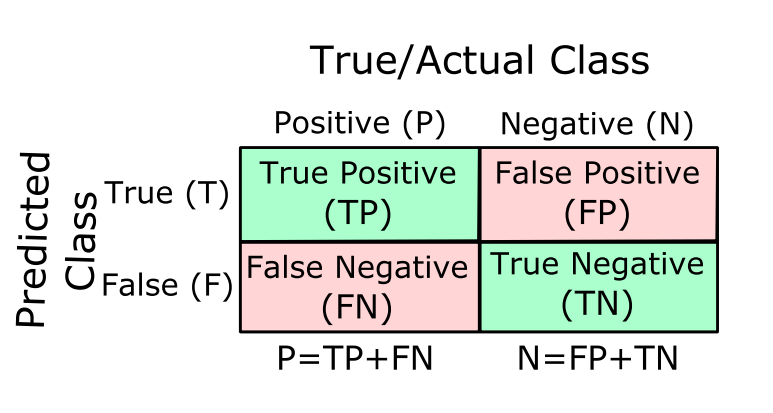
\includegraphics[scale=0.5]{gambar/confusionmatrix.png}
  \caption{Contoh \emph{Confusion Matrix} dengan dimensi 2 x 2 (Tharwat, 2018)}
  \label{fig:confusionmatrixex}
\end{figure}

Ada dua jenis masalah klasifikasi: klasifikasi biner dengan dua kelas dan klasifikasi multi-kelas dengan lebih dari dua kelas. Dalam klasifikasi biner, sampel diklasifikasikan sebagai positif (P) atau negatif (N). Model klasifikasi yang dilatih dalam fase pelatihan digunakan untuk memprediksi kelas sebenarnya dari sampel yang tidak diketahui, menghasilkan keluaran yang terpisah atau kontinu. Keluaran diskrit mewakili label kelas yang diprediksi, sedangkan keluaran kontinu menunjukkan probabilitas keanggotaan kelas yang diperkirakan. Matriks kontinjensi atau tabel kontinjensi dengan empat kemungkinan keluaran digunakan untuk mengevaluasi kinerja klasifikasi. Diagonal hijau mewakili prediksi yang benar, sedangkan diagonal merah muda mewakili prediksi yang salah. True positive (TP) adalah sampel positif yang diklasifikasikan dengan benar, false negative (FN) adalah sampel negatif yang salah diklasifikasikan sebagai positif, true negative (TN) adalah sampel negatif yang diklasifikasikan dengan benar, dan false positive (FP) adalah sampel positif yang salah diklasifikasikan sebagai negatif. Matriks konfusi digunakan untuk menghitung berbagai metrik klasifikasi (Tharwat, 2018).

\subsection{\emph{Recall}}
\label{subsec:cnn}

Penarikan kembali suatu pengklasifikasi menunjukkan rasio sampel positif yang diklasifikasikan dengan benar terhadap jumlah total sampel positif. Di sisi lain, spesifisitas, juga dikenal sebagai true negative rate (TNR) atau inverse recall, dihitung dengan membagi jumlah sampel negatif yang diklasifikasikan dengan benar dengan jumlah total sampel negatif. Oleh karena itu, spesifisitas mewakili proporsi sampel negatif yang diklasifikasikan secara akurat, sedangkan sensitivitas mengacu pada proporsi sampel positif yang diklasifikasikan dengan benar (Tharwat, 2018).

\begin{equation}
  \label{eq:KonversiPanjangLangkah}
  \emph{Precision} = \frac{TP}{TP + FN}
\end{equation}

\subsection{\emph{Precision}}
\label{subsec:cnn}

Presisi adalah ukuran yang menghitung rasio sampel positif yang diklasifikasikan dengan benar terhadap jumlah total sampel yang diprediksi positif. Sebaliknya, Nilai Prediktif Negatif (NPV), juga dikenal sebagai presisi terbalik atau True Negative Accuracy (TNA), mengkuantifikasi proporsi sampel negatif yang diklasifikasikan dengan benar ke jumlah total sampel prediksi negatif. Penting untuk dicatat bahwa kedua ukuran ini dipengaruhi oleh data yang tidak seimbang (Tharwat, 2018).

\begin{equation}
  \label{eq:KonversiPanjangLangkah}
  \emph{Precision} = \frac{TP}{TP + FP}
\end{equation}

\subsection{\emph{F-Measure}}
\label{subsec:cnn}

F-measure, juga dikenal sebagai F1-score, adalah metrik yang menghitung rata-rata harmonik presisi dan perolehan. Nilai ukuran-F berkisar dari nol hingga satu, di mana nilai yang lebih tinggi menunjukkan kinerja klasifikasi yang lebih baik. Variasi lain dari pengukuran ini adalah pengukuran F, yang mewakili rata-rata harmonik tertimbang dari presisi dan daya ingat. Penting untuk diperhatikan bahwa metrik ini sensitif terhadap perubahan distribusi data (Tharwat, 2018).

\begin{equation}
  \label{eq:KonversiPanjangLangkah}
  F-Measure = \frac{2 (\emph{precision}\times\emph{recall})}{\emph{precision} + \emph{recall}}
\end{equation}

\subsection{\emph{Error}}
\label{subsec:cnn}

Kesalahan mengacu pada perbedaan persentase antara nilai yang diharapkan atau diprediksi dan hasil aktual. Persentase kesalahan umumnya digunakan untuk menilai keakuratan model peramalan dalam perhitungan tertentu (Deepthi et al., 2017).

\begin{equation}
  \label{eq:KonversiPanjangLangkah}
  \emph{Error} = \frac{nilai \; sebenarnya - nilai \; terukur}{nilai \; sebenarnya} \times 100\%
\end{equation}

\subsection{\emph{Accuracy}}
\label{subsec:cnn}

Akurasi adalah metrik yang digunakan untuk mengevaluasi kinerja model dalam mengklasifikasikan atau memprediksi dataset tertentu. Ini ditentukan dengan membandingkan jumlah prediksi yang benar yang dibuat oleh model dengan jumlah total contoh data yang diuji (Deepthi et al., 2017).

\begin{equation}
  \label{eq:KonversiPanjangLangkah}
  \emph{Accuracy} =  100\% - \%Error
\end{equation}
\cleardoublepage

% Bab 3 desain dan implementasi
\chapter{DESAIN DAN IMPLEMENTASI}
\label{chap:desainimplementasi}

Penelitian ini dilaksanakan sesuai sistem berikut dengan implementasinya. Desain sistem merupakan konsep dari pembuatan dan perancangan infrastuktur yang kemudian diwujudkan dalam bentuk blok diagram alur yang harus dikerjakan. Pada bagian implementasi merupakan pelaksanaan teknis untuk setiap blok pada desain sistem. Pada Gambar 3.1 menunjukan bagan umum metodologi sistem.

\begin{figure}[H]
  \centering
  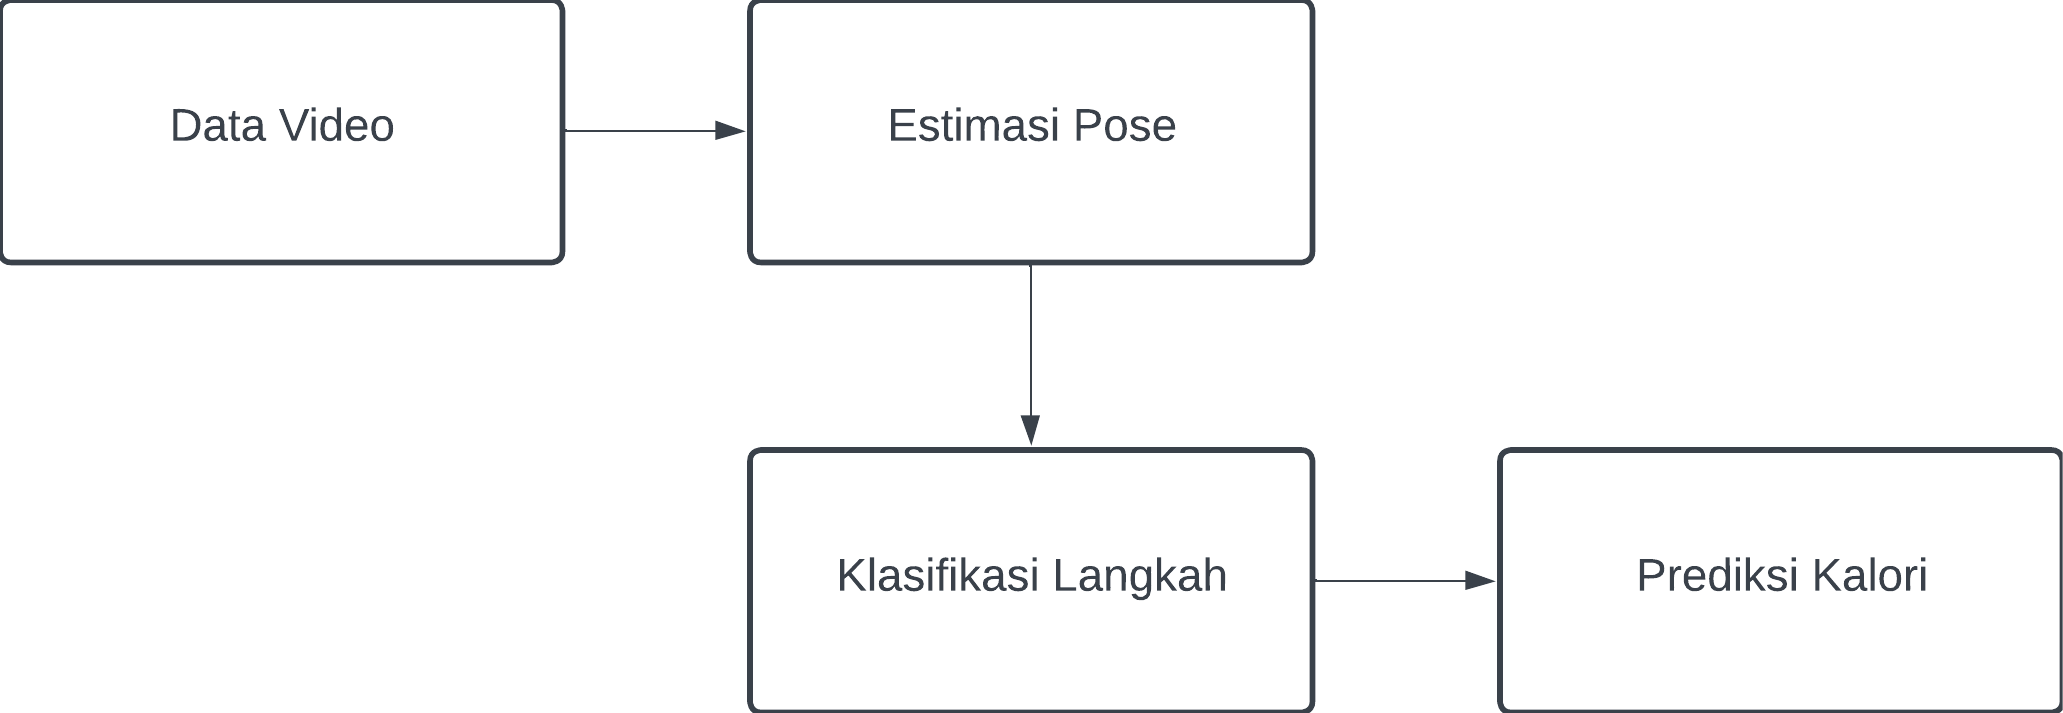
\includegraphics[scale=0.215]{gambar/blok diagram metodologi4.png}
  \caption{Blok Diagram Kerja Sistem}
  \label{fig:BlokDiagram}
\end{figure}

Berdasarkan Gambar \ref{fig:BlokDiagram} dalam menjelaskan alur kerja sistem yang digunakan dimulai dengan \emph{input} yang berupa data video menghasilkan beberapa data video yang akan digunakan dan diproses dengan melakukan estimasi pose dan klasifikasi langkah. Pada estimasi pose data video akan diestimasi pose untuk didapatkan hasil berupa dataset yang telah diekstrak fitur untuk dilakukan klasifikasi langkah. Klasifikasi langkah dilakukan dengan menggunakan model dari dataset yang dibuat dengan menggunakan arsitektur CNN untuk mendeteksi langkah. Hasil yang didapat dari proses klasifikasi langkah berupa banyak langkah dan waktu tempuh untuk dilakukan proses prediksi kalori. Prediksi kalori dilakukan dengan dua cara yaitu regresi dan perhitungan rumus. Hasil \emph{output} dari sistem ini adalah hasil prediksi kalori yang terbakar dari data video yang digunakan.

\section{Data Video}
\label{sec:PengambilanData}

Pada penelitian ini digunakan data berupa data video yang dilakukan pengambilan data dan diperoleh menggunakan kamera pada \emph{smartphone} yang akan direkam dan disimpan untuk kemudian akan digunakan pada proses yang dilakukan pada perangkat komputer/laptop atau dapat menggunakan kamera yang dimiliki oleh laptop atau kamera eksternal yang dihubungkan pada laptop ataupun komputer. Proses pengambilan data dilakukan dengan peraga melakukan aktivitas pada treadmill dengan ditampakkan secara jelas pada tampilan kamera. Setelah terdapat peraga dan tampak jelas pada tampilan maka data citra akan dilakukan pada tahap selanjutnya untuk dideteksi dan segmentasi pose seperti pada Gambar \ref{fig:DataVideo}.

\begin{figure}[H]
  \centering
  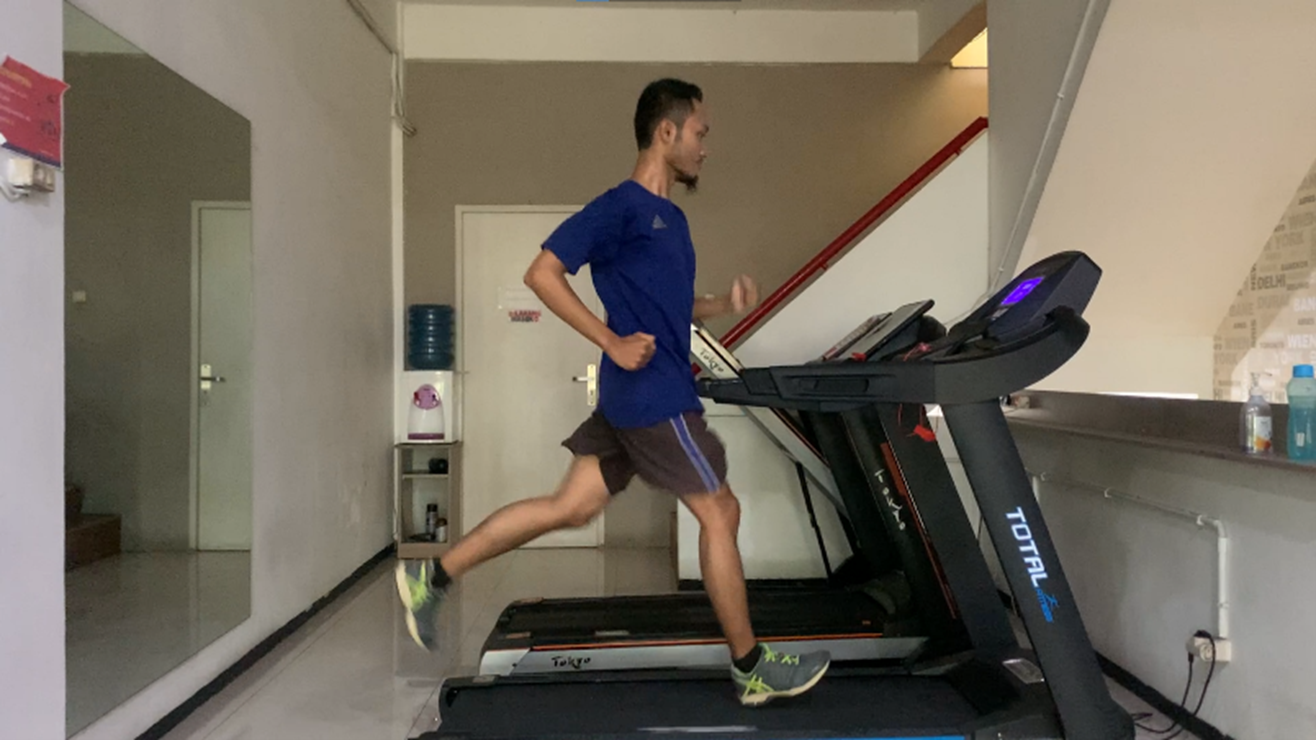
\includegraphics[scale=0.8]{gambar/pengambilan data.png}
  \caption{Proses pengambilan data}
  \label{fig:DataVideo}
\end{figure}

Data video yang digunakan pada penelitian ini berdasarkan pengambilan data video yang telah dilakukan. Pengambilan data dilakukan pada aktivitas yang dilakukan pada treadmill. Variasi yang digunakan pada data video yang digunakan berdasarkan variasi kecepatan dan hasil kalori yang terbakar. Tabel \ref{tb:DatasetVideo} menunjukkan data video berdasarkan variasi yang digunakan.

\begin{longtable}{|c|c|c|}
  \caption{Data video berdasarkan pengambilan data}
  \label{tb:DatasetVideo}  \\
  \hline
  \rowcolor[HTML]{C0C0C0}
  \textbf{Percobaan} & \textbf{Kecepatan} & \textbf{Kalori Terbakar} \\
  \hline
  1     & 3     & 10   \\
  \hline
  2     & 6     & 10   \\
  \hline
  3     & 9     & 20   \\
  \hline
  4     & 12    & 20   \\
  \hline
  5     & 8     & 20   \\
  \hline
  7     & 12    & 20   \\
  \hline
\end{longtable}


\section{Estimasi Pose}
\label{sec:EstimasiPose}

Estimasi dari hasil citra untuk dapat mengetahui bentuk postur tubuh manusia menggunakan Python dengan \emph{library} OpenCV yaitu MediaPipe. Metode yang digunakan pada MediaPipe menggunakan estimasi pose untuk mendeteksi postur tubuh. Segementasi dilakukan dengan cara peraga melakukan aktivitas jogging pada treadmill dengan menentukan pose melangkah ataupun berlari sesuai dengan olahraga yang akan diteliti. Data yang diproses merupakan data yang telah dilakukan perekaman pada proses pengambilan data dengan menggunakan video yang telah direkam sebelumnya menggunakan alat perekam. Hasil video yang memperlihatkan seseorang dalam keadaan berolahraga pada treadmill melakukan aktivitas berjalan atau berlari akan diproses dalam tahap ini untuk dilakukan estimasi pose. Estimasi pose menggunakan model Estimasi yang sudah ada yaitu Mediapipe. Hasil estimasi dari model Mediapipe berupa kerangka yang menyesuaikan bentuk tubuh yang diestimasi dari data video yang dimiliki.

Dalam penelitian ini yang berfokuskan pada proses deteksi langkah pada tubuh bagian bawah seperti kaki menyebabkan perlunya pemodelan ulang dan melakukan proses modifikasi pada hasil estimasi model Mediapipe. Dengan begitu proses modifikasi yang dilakukan adalah dengan mengambil kerangka bagian kaki dengan memberikan warna yang berbeda untuk hasil estimasi kaki bagian kiri dan kanan. Proses estimasi pose pada kaki yang dilakukan akan digunakan dalam proses selanjutnya dalam penelitian ini yang digambarkan pada gambar yang terdapat pada Gambar \ref{fig:DeteksiEstimasi}.

\begin{figure}[H]
  \centering
  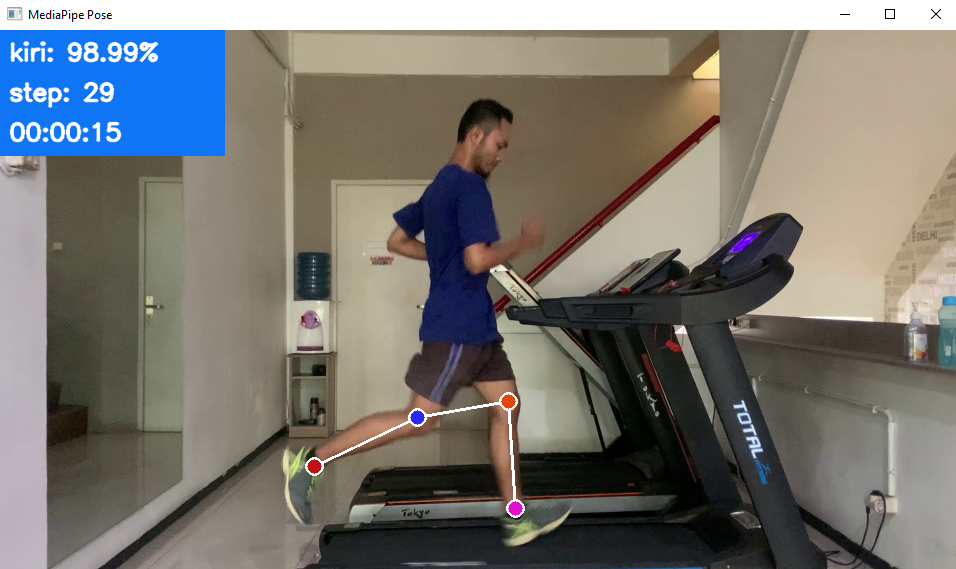
\includegraphics[scale=0.45]{gambar/deteksi pose.png}
  \caption{Deteksi pose dengan MediaPipe}
  \label{fig:DeteksiEstimasi}
\end{figure}

\subsection{\emph{Preprocessing} Data}
\label{subsec:PreProcessingData}

Hasil estimasi pose dengan bentuk kerangka pada kaki sesuai dengan data video dilakukan tahap \emph{preprocessing}. \emph{Preprocessing} data dilakukan sebagai proses untuk mempersiapkan data dari input yang digunakan untuk kemudian dilakukannya proses pembuatan model dalam tahap \emph{training}. Terdapat beberapa tahapan yang dilakukan pada \emph{preprocessing} data untuk kemudian akan didapatkan dataset yang akan dapat digunakan untuk melakukan pembuatan model dengan proses \emph{training}. Setiap data video yang akan digunakan dalam proses ini akan dilakukan ekstrak dari data video menjadi gambar. Data video yang memiliki resolusi sebesar 1920 x 1080 dengan 25 FPS akan diubah dan diekstrak menjadi satuan gambar untuk digunakan sebagai dataset melalui proses \emph{preprocessing} data. Dengan resolusi data demikian akan menghasilkan 25 gambar atau \emph{frame} setiap satu detik dari video tersebut. Hasil ekstrak gambar dalam \emph{preprocessing} data ini akan kemudian dilanjutkan dalam proses untuk membuat dataset untuk kemudian digunakan dalam proses \emph{training} menjadi model.

\subsection{Ekstrak Fitur}
\label{subsec:AugmentasiData}

Pada proses estimasi pose didapat hasil estimasi pada data video berupa kerangka pada kaki yang menyesuaikan bentuk tubuh yang sedang ditampilkan. Setelah dapat diestimasi dengan baik menggunakan model Mediapipe dan dimodifikasi untuk dapat terfokus pada bagian kaki, dilakukan proses ekstrak fitur. Ekstrak fitur dilakukan sebagai proses untuk mengubah atau memodifikasi gambar agar dapat dengan mudah diproses dalam tahap \emph{training}. Proses ini juga akan dapat membantu dalam meningkatkan akurasi dari model yang akan digunakan nanti karena data telah diproses dan dimodifikasi agar memiliki data-data tambahan yang akan berguna dalam tahap \emph{training}. Data dari proses estimasi pose akan dilakukan proses pemindahan hasil estimasi kerangka ke dalam gambar baru dengan penyesuaian yang akan digeneralisasikan terhadap semua data yang didapat. 

Proses dimulai dengan menentukan posisi kerangka dari data video asli untuk kemudian akan dipindahkan ke gambar baru. Dalam melakukan menentukan posisi kerangka dilakukan dengan estimasi menggunakan bingkai yang menyesuaikan posisi keseluruhan kerangka yang dapat dilihat pada Gambar \ref{fig:PreProcessing1}. Setelah bingkai menyesuaikan posisi kerangka maka akan dipindahkan pada gambar dengan latar belakang hitam yang berisikan hanya kerangka dari hasil estimasi sesuai dengan bingkai. Proses melakukan pemindahan hasil estimasi ke dalam gambar dengan latar belakang hitam dapat ditunjukan pada gambar Gambar \ref{fig:PreProcessing2}. Kemudian gambar akan dilakukan generalisasi terhadap ukuran yang berisikan hanya hasil estimasi sesuai bingkai untuk mempermudah dalam proses selanjutnya dengan membuat ukuran gambar seragam dalam bentuk persegi.

\begin{figure}[H]
  \centering
  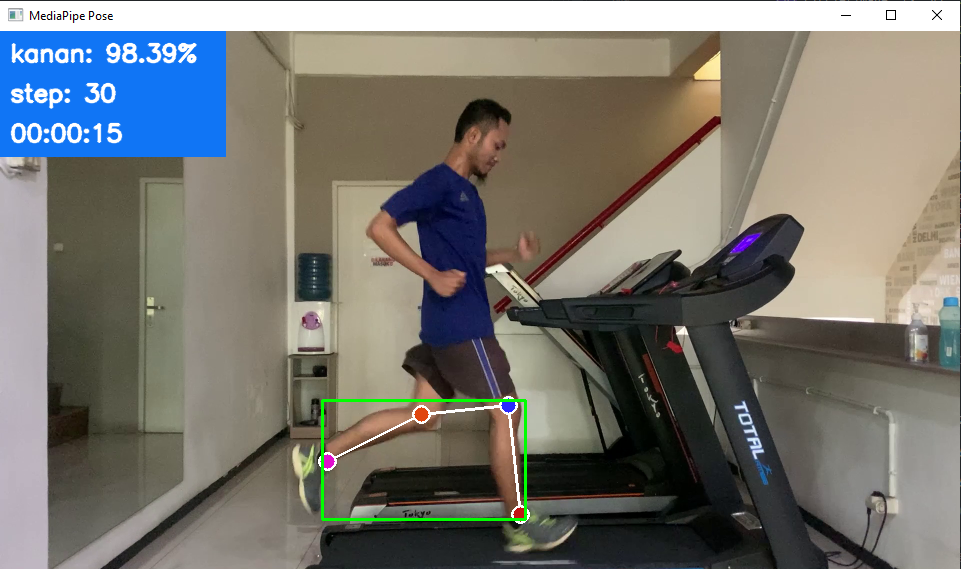
\includegraphics[scale=0.48]{gambar/deteksi pose2.png}
  \caption{\emph{Preprocessing} hasil estimasi pose dengan bingkai}
  \label{fig:PreProcessing1}
\end{figure}

\begin{figure}[H]
  \centering
  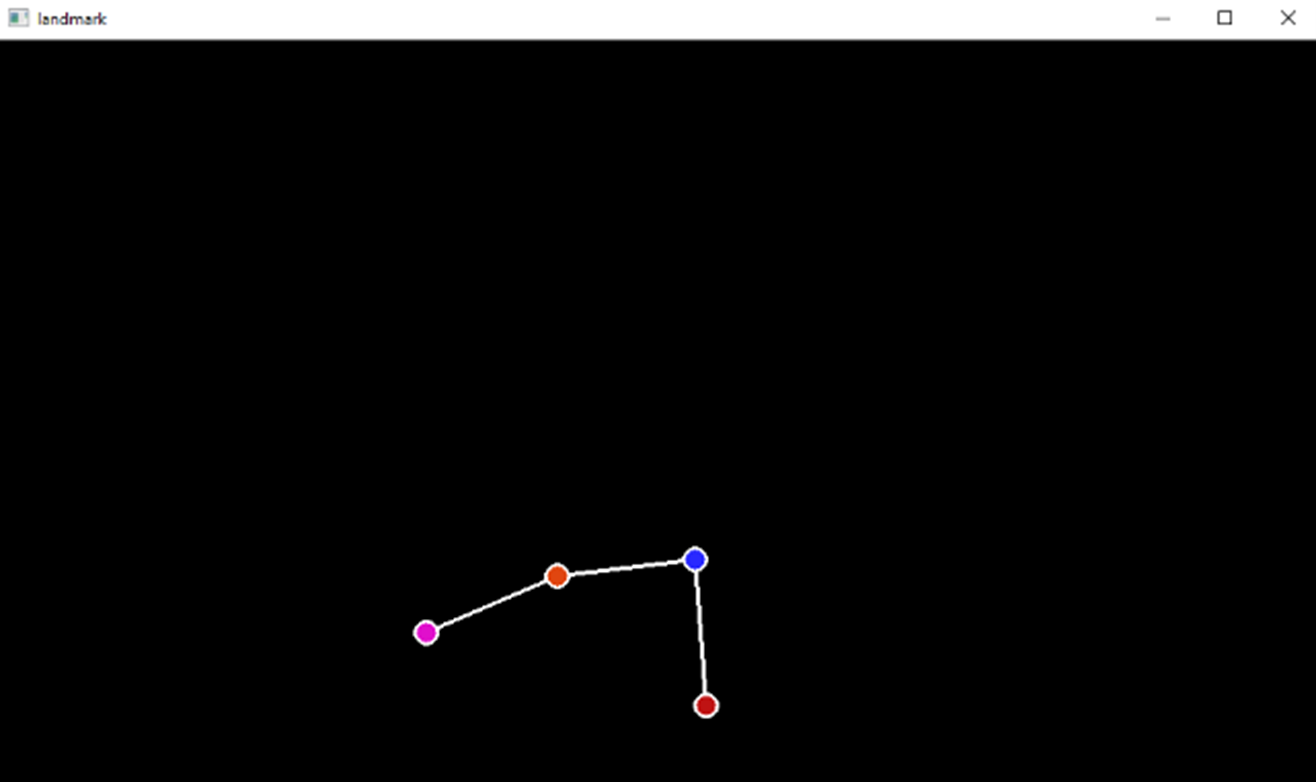
\includegraphics[scale=0.8]{gambar/deteksi pose3.png}
  \caption{\emph{Preprocessing} hasil estimasi pose pada latar belakang hitam}
  \label{fig:PreProcessing2}
\end{figure}

\subsection{Pelabelan Objek}
\label{subsec:PelabelanObjek}

Hasil dari proses ekstrak fitur dengan melakukan pemindahan hasil estimasi ke dalam gambar baru yang telah disesuaikan akan diproses menjadi sebuah dataset. Pelabelan objek diperlukan untuk dapat memberikan informasi nama kelas dari objek yang akan dideteksi pada penelitian ini. Proses pada pelabelan objek ini dilakukan setelah didapatkan proses dalam \emph{preprocessing} dengan mengekstrak data video menjadi gambar dan dilakukan proses ekstrak fitur dari setiap data gambar yang didapat. Kemudian dari hasil ekstrak fitur dengan memiliki hasil gambar kerangka berdasarkan hasil deteksi dikelompokkan pada kategori atau kelas yang berbeda. Pada penelitian ini proses deteksi yang diinginkan adalah dapat menentukan proses aktivitas melangkah atau berlari dengan mengetahui kaki kanan atau kiri yang sedang berada di depan. Dengan begitu kelas yang dimiliki pada dataset yang akan dibuat dengan terdapat dua label atau kelas yaitu kanan dan kiri. Hasil ekstraksi dan ekstrak fitur yang dilakukan berdasarkan kelas yang diinginkan dapat dilihat untuk kelas kanan pada Gambar \ref{fig:KelasKanan} dan untuk kelas kiri pada Gambar \ref{fig:KelasKiri}. Dari setiap gambar yang telah dilakukan ekstraksi fitur dilakukan pemberian label sesuai dengan kelas yang akan digunakan. Hasil pelabelan objek gambar tersebut ditunjukkan pada Tabel \ref{tb:HasilAnotasi}.

\begin{figure}[H]
  \centering
  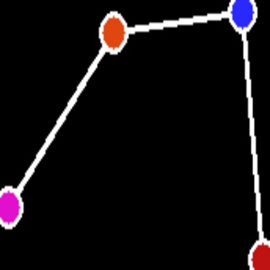
\includegraphics[scale=0.8]{gambar/dataset kanan.png}
  \caption{Hasil \emph{preprocessing} untuk kelas kanan}
  \label{fig:KelasKanan}
\end{figure}

\begin{figure}[H]
  \centering
  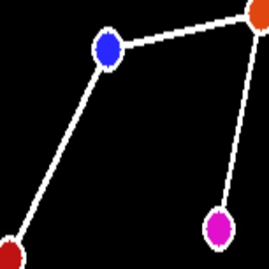
\includegraphics[scale=0.8]{gambar/dataset kiri.png}
  \caption{Hasil \emph{preprocessing} untuk kelas kiri}
  \label{fig:KelasKiri}
\end{figure}

\begin{longtable}{|c|c|}
  \caption{Hasil anotasi dari pelabelan objek}
  \label{tb:HasilAnotasi}  \\
  \hline
  \rowcolor[HTML]{C0C0C0}
  \textbf{Kelas} & \textbf{Jumlah Anotasi}  \\
  \hline
  Kanan           & 888    \\
  \hline
  Kiri            & 843    \\
  \hline
  \textbf{Total}  & 1.731  \\
  \hline
\end{longtable}


\subsection{Dataset}
\label{subsec:Dataset}

Dataset yang digunakan pada penelitian ini berdasarkan hasil dari data video yang dimiliki dengan mengambil sampel pada proses pengambilan data. Kemudian dilakukan proses \emph{preprocessing} dengan melakukan ekstraksi gambar, augmentasi data, dan pelabelan objek yang akan disimpan keseluruhan data yang dimiliki berdasarkan kelas untuk menjadi dataset yang akan digunakan pada penelitian ini. Dataset yang telah dimiliki pada penelitian ini berupa data gambar berisikan bentuk kerangka dari hasil deteksi dengan model Mediapipe yang telah dimodifikasi dan digeneralisasi untuk ukuran gambar. Hasil dari dataset yang akan digunakan untuk dataset kelas kanan ditunjukkan pada Gambar \ref{fig:DatasetKanan} dan untuk dataset kelas kiri ditunjukkan pada Gambar \ref{fig:DatasetKiri}.

\begin{figure}[H]
  \centering
  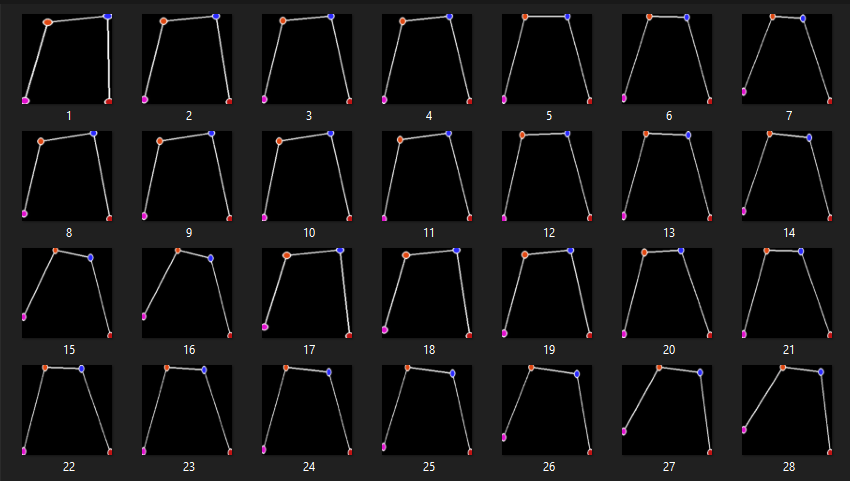
\includegraphics[scale=0.45]{gambar/folder dataset kanan.png}
  \caption{Dataset untuk kelas Kanan}
  \label{fig:DatasetKanan}
\end{figure}

\begin{figure}[H]
  \centering
  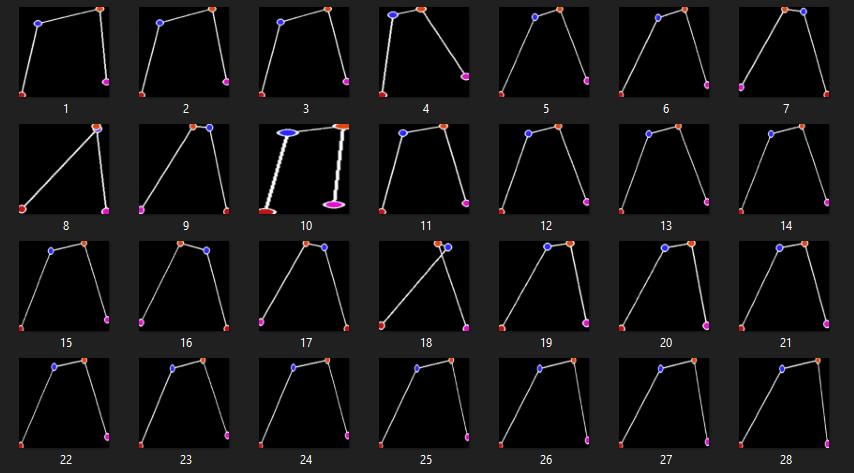
\includegraphics[scale=0.45]{gambar/folder dataset kiri.png}
  \caption{Dataset untuk kelas Kiri}
  \label{fig:DatasetKiri}
\end{figure}


\section{Klasifikasi Langkah}
\label{sec:Klasifikasi}

Dataset yang telah dimiliki maka kemudian dilakukan \emph{training} untuk memperoleh model deteksi. Model deteksi dari dataset akan digunakan untuk melatih model dari sebuah algoritma pada \emph{Machine Learning}. Dalam melakukan klasifikasi menggunakan \emph{Convolutional Neural Networks} (CNN). Proses \emph{training} ini bertujuan agar nantinya komputasi yang dilakukan dalam proses deteksi akan dapat diolah berdasarkan akuisisi data citra yang ingin dideteksi menjadi bentuk atau pola pemahaman yang diinginkan. Hasil \emph{training} akan didapatkan model yang digunakan untuk melakukan klasifikasi atas dataset yang dimiliki yaitu terdapat dua kelas atau label untuk dapat diklasifikasikan menjadi kaki kanan dan kiri. Klasifikasi dalam menentukan aktivitas yang digunakan pada penelitian ini adalah dapat mengetahu langkah dari seseorang yang berjalan atau berlari. Hasil klasifikasi dari model yang telah dibuat untuk menentukan hasil deteksi untuk kelas kanan ditunjukkan pada Gambar \ref{fig:KlasifikasiKanan} dan hasil deteksi untuk kelas kiri ditunjukkan pada Gambar \ref{fig:KlasifikasiKiri}.

\begin{figure}[H]
  \centering
  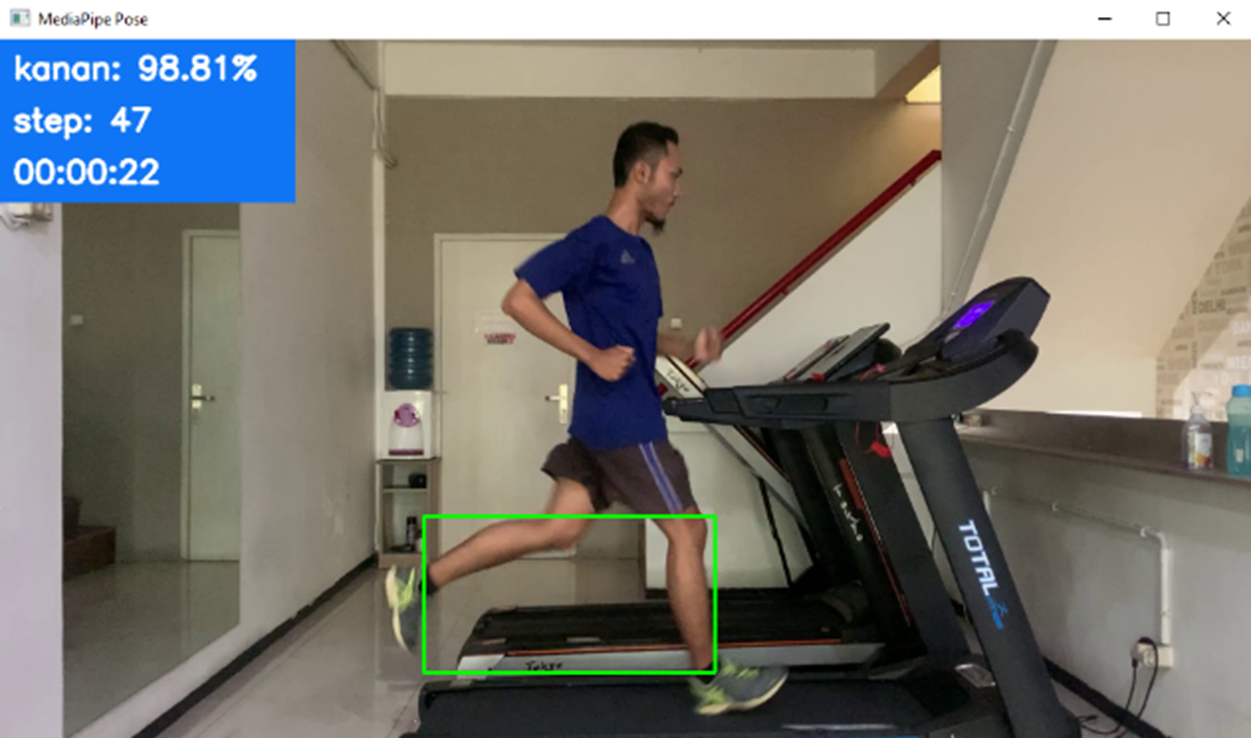
\includegraphics[scale=0.8]{gambar/klasifikasi kanan.png}
  \caption{Klasifikasi untuk kelas kanan}
  \label{fig:KlasifikasiKanan}
\end{figure}

\begin{figure}[H]
  \centering
  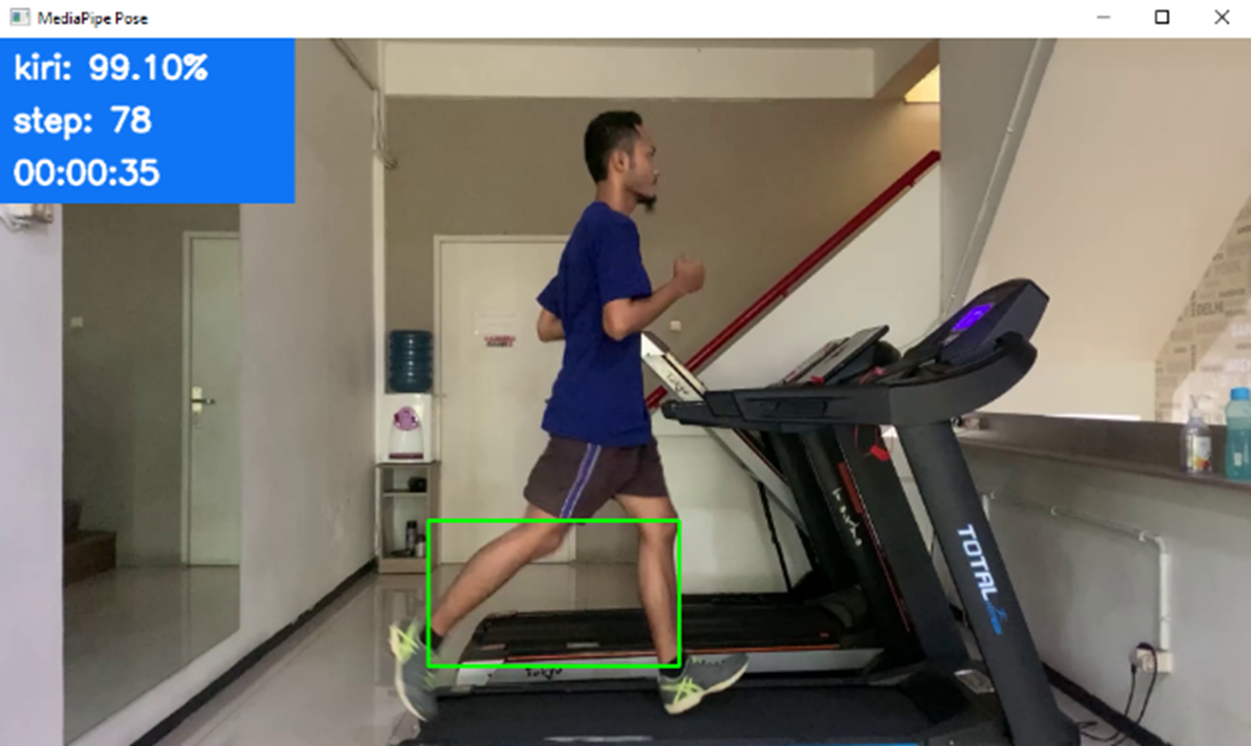
\includegraphics[scale=0.8]{gambar/klasifikasi kiri.png}
  \caption{Klasifikasi untuk kelas kiri}
  \label{fig:KlasifikasiKiri}
\end{figure}


\subsection{Hasil Deteksi}
\label{subsec:HasilDeteksi}

Bentuk hasil klasifikasi yang dibuat adalah mendeteksi pose aktivitas dengan dapat menghitung langkah dan waktu yang ditempuh. Nilai langkah dan waktu yang ditempuh akan digunakan dalam perhitungan selanjutnya. Banyaknya jumlah langkah yang didapat saat hasil deteksi digunakan sebagai nilai variable pertama yang akan digunakan dalam penentuan perhitungan kalori. Langkah dideteksi dan dihitung seberapa banyak langkah yang dilakukan saat proses deteksi. Waktu tempuh saat proses deteksi merupakan nilai variabel kedua yang akan digunakan dalam penentuan perhitungan kalori. Waktu tempuh dimulai saat dideteksi pertama kali nilai langkah yang ditemukan hingga saat akhir langkah tidak ada penambahan kembali yang menandakan proses deteksi telah selesai. Hasil deteksi akan ditampilkan seiring dengan proses deteksi yang dilakukan pada data citra seperti pada Gambar \ref{fig:HasilDeteksi} dan pada akhir proses deteksi akan menampilkan hasil akumulasi akhir dari hasil deteksi terhadap deteksi langkah dan waktu tempuh. Selain itu juga terdapat tampilan hasil perhitungan dan prediksi yang diharapkan dalam penelitian ini. Hasil tampilan untuk hasil deteksi di akhir sebagai akumulasi deteksi ditunjukkan pada Gambar \ref{fig:HasilDeteksi2}.

\begin{figure}[H]
  \centering
  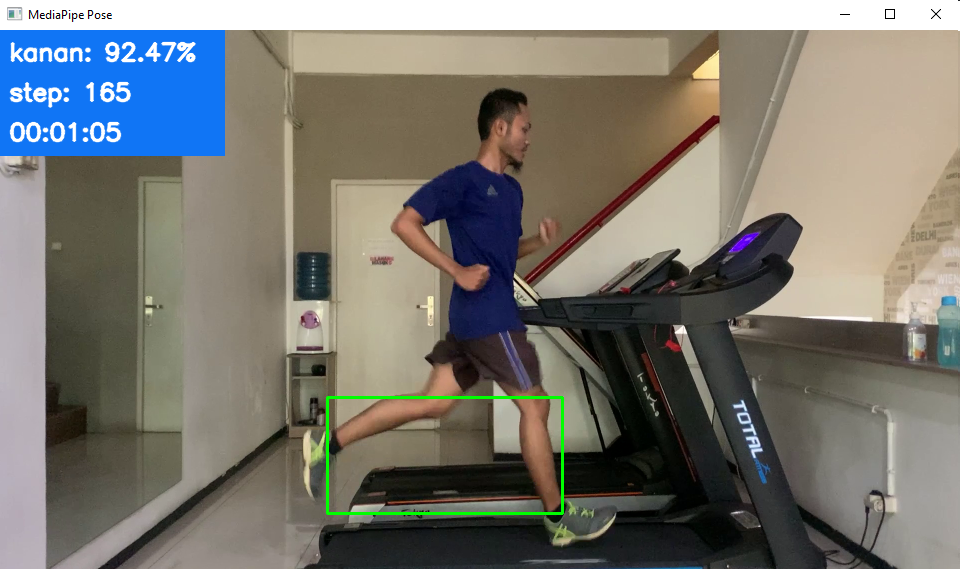
\includegraphics[scale=0.48]{gambar/hasil deteksi.png}
  \caption{Tampilan hasil deteksi saat proses deteksi}
  \label{fig:HasilDeteksi}
\end{figure}

\begin{figure}[H]
  \centering
  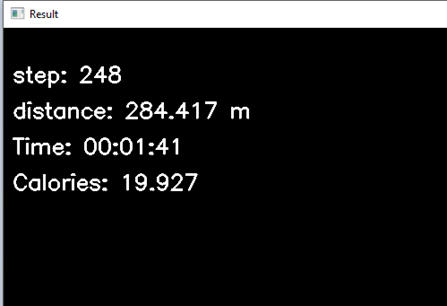
\includegraphics[scale=0.7]{gambar/hasil deteksi2.png}
  \caption{Tampilan akumulasi hasil deteksi}
  \label{fig:HasilDeteksi2}
\end{figure}

\subsection{Hasil Deteksi Langkah}
\label{subsec:HasilLangkah}

Banyaknya jumlah langkah yang didapat saat hasil deteksi digunakan sebagai nilai variable pertama yang akan digunakan dalam penentuan perhitungan kalori. Langkah dideteksi dan dihitung seberapa banyak langkah yang dilakukan saat proses deteksi. Dalam proses deteksi menggunakan model yang sudah dibuat mendapatkan hasil deteksi sesuai kelas yang digunakan yaitu kanan dan kiri. Saat sistem berhasil mendeteksi langkah berdasarkan model langkah kanan dan kiri akan melakukan akumulasi perhitungan langkah dengan menjumlahkan banyak hasil deteksi saat mengalami perubahan hasil deteksi. Dengan adanya perubahan hasil deteksi dari kelas kanan menjadi kiri ataupun sebaliknya, maka sistem akan melakukan penjumlahan pada variabel jumlah langkah berdasarkan hasil deteksi yaitu langkah dengan menggunakan deteksi langkah dari model yang telah dibuat. Saat dideteksinya awal langkah dan perubahan langkah yang mengakibatkan bertambahnya jumlah akumulasi langkah yang dideteksi akan membuat sistem berjalan dan membuat waktu tempuh dimulai berdasarkan hasil langkah awal yang dapat dideteksi. Proses deteksi langkah akan dimulai dengan dimulainya akuisisi data maupun berdasarkan dari data citra dataset dan diakhiri dengan akhir dari deteksi langkah yang tidak mengalami pertambahan dalam kurung waktu tertentu. Hasil akumulasi jumlah langkah akan disimpan dan dilakukan proses selanjutnya dalam menentukan prediksi dan perhitungan kalori.

\subsection{Hasil Waktu Tempuh}
\label{subsec:HasilWaktu}

Waktu tempuh saat proses deteksi merupakan nilai variabel kedua yang akan digunakan dalam penentuan perhitungan kalori. Waktu tempuh dimulai saat dideteksi pertama kali nilai langkah yang ditemukan hingga saat akhir langkah tidak ada penambahan kembali yang menandakan proses deteksi telah selesai. Nilai waktu yang akan digunakan selanjutnya merupakan nilai waktu dalam bentuk satuan detik hasil dari akumulasi keseluruhan dalam proses deteksi. Pada tampilan hasil deteksi waktu tempuh ditampilkan dalam keseluruhan satuan waktu berupa jam, menit dan detik yang dapat dilakukan akumulasi berdasarkan proses melakukan deteksi dari hasil akuisisi data maupun berdasarkan dari data citra dataset. Hasil akumulasi dari satuan detik yang didapat akan disimpan dan dilakukan pada proses selanjutnya dalam menentukan prediksi dan perhitungan kalori.

\section{Prediksi Kalori}
\label{sec:PrediksiKalori}

Prediksi kalori dilakukn dengan dua metode, yaitu menggunakan metode regresi linear dan menggunakan perhitungan rumus EC (Exercise Calories) berdasarkan satuan ukuran MET (Metabolic Equivalent). Kedua metode prediksi ini digunakan sebagai pembanding dalam melakukan analisa terhadap hasil yang didapatkan dari metode prediksi menggunakan metode regresi linear dengan perhitungan rumus. Data yang digunakanan dalam proses prediksi kalori diambil berdasarkan hasil klasifikasi dan hasil deteksi yang telah dilakukan sebelumnya. Hasil deteksi berupa banyaknya langkah dan waktu tempuh digunakan untuk proses prediksi kalori baik dengan metode regresi linear maupun metode perhitungan rumus.

\subsection{Regresi Linear}
\label{subsec:PrediksiRegresi}

Prediksi kalori dengan regresi linear dilakukan dengan teknik analisis untuk mengidentifikasi relasi antar dua variabel atau lebih. Pada penelitian ini varibel yang digunakan adalah hasil deteksi berupa hasil jumlah deteksi langkah dengan hasil waktu tempuh untuk nantinya akan dicari terkait relasi antara variabel tersebut untuk bisa menentukan hasil yang diinginkan yaitu prediksi kalori. Dalam memulai melakukan proses regresi linear untuk prediksi kalori, dilakukan proses pengambilan data untuk diolah menjadi dataset yang akan digunakan dalam beberapa proses pada prediksi kalori dengan regresi linear ini. Proses pengambilan data dilakukan pada alat treadmill yang dilakukan uji dengan beragam variasi dan dilakukan pencatatan data untuk digunakan sebagai dataset pada penelitian ini. Data yang diambil untuk dilakukan pengolahan dari alat treadmill adalah data waktu, kecepatan dan kalori terbakar. Data yang diperoleh dengan mengumpulkan data untuk model regresi linear dari alat treadmill didapatkan jumlah 1045 total data yang dapat dilihat pada Tabel \ref{tb:DatasetRegresi}

\begin{longtable}{|c|c|c|c|}
  \caption{Hasil pengambilan data pada treadmill}
  \label{tb:DatasetRegresi}                                   \\
  \hline
  \rowcolor[HTML]{C0C0C0}
  \textbf{No} & \textbf{Waktu} & \textbf{Kecepatan} & \textbf{Kalori Terbakar} \\
  \hline
  1   & 0:06    & 1 (km/j)    & 0,1     \\
  \hline
  2   & 0:11    & 1 (km/j)    & 0,2     \\
  \hline
  54   & 0:50    & 2 (km/j)    & 1,9     \\
  \hline
  55   & 0:53    & 2 (km/j)    & 2,0     \\
  \hline
  215   & 1:03    & 3 (km/j)    & 3,6     \\
  \hline
  216   & 1:05    & 3 (km/j)    & 3,7     \\
  \hline
  375   & 1:18    & 4 (km/j)    & 6,0     \\
  \hline
  376   & 1:19    & 4 (km/j)    & 6,1     \\
  \hline
  700   & 1:43    & 8 (km/j)    & 16,0     \\
  \hline
  701   & 1:44    & 8 (km/j)    & 16,2     \\
  \hline
  1044   & 2:26    & 12 (km/j)    & 34,1     \\
  \hline
  1045   & 2:27    & 12 (km/j)    & 34,4     \\
  \hline
\end{longtable}

Untuk dapat melakukan prediksi kalori dari hasil deteksi yang didapat menggunakan regresi linear diperlukan model regresi berdasarkan pemodelan dataset yang dibuat terlebih dahulu dan nantinya saat model regresi telah didapat maka akan dapat melakukan prediksi kalori berdasarkan akuisisi maupun dataset untuk dilakukan proses prediksi dengan regresi linear. Dalam melakukan prediksi kalori dengan melakukan pemodelan regresi dilakukan dengan beberapa tahap untuk memproses hasil deteksi sehingga dapat melakukan prediksi. Tahapan untuk membuat model regresi yang diinginkan sesuai model sistem pada penelitian ini adalah dengan membuat regresi jarak tempuh, dataset regresi prediksi kalori dan model regresi linear prediksi kalori.

Tahap pertama dalam melakukan prediksi kalori dari hasi deteksi yang sudah didapat diperlukan untuk melakukan pengolahan data dari hasil deteksi menjadi suatu variabel yang dapat digunakan dalam membuat model regresi. Hasil deteksi berupa banyak langkah dan waktu tempuh diolah agar dapat menjadi variabel dalam membuat model regresi prediksi kalori yang nantinya akan mempermudah dalam data yang didapat saat akuisisi dari hasil deteksi yaitu jarak tempuh dan waktu tempuh. Jarak tempuh pada model regresi prediksi kalori ini didapatkan dengan menggunakan rumus mencari jarak berdasarkan waktu dan kecepatannya yang ditunjukkan pada Persamaan \ref{eq:JarakTempuh}

\begin{equation}
  \label{eq:JarakTempuh}
  Jarak Tempuh = \frac{Kecepatan}{Waktu}
\end{equation}

Dengan menggunakan rumus jarak tempuh berdasarkan kecepatan dan waktu, maka data yang telah dilakupan pengumpulan data untuk regresi linear pada alat treadmil dapat dilakukan pengolahan pada data kecepatan untuk menggunakan jarak tempuh agar mempermudah dalam proses sistem untuk mengenali data berdasarkan hasil deteksi pada penelitian ini. Dari setiap data yang dilakukan pengumpulan data dengan jumlah total data sebanyaka 1045 data akan dilakukan pengolahan untuk nantinya akan menggunakan data waktu tempuh dalam satuan detik, jarak tempuh dalam meter dan kalori yang terbakar. Menentukan jarak tempuh dalam meter dengan menggunakan data berupa waktu dengan satuan menit dan detik lalu kecepatan dalam satuan kilometer per jam dapat melakukan konversi satuan nilai dan menghasilkan persamaan untuk mengubah nilai tersebut sesuai yang diinginkan dan ditunjukkan pada Persamaan \ref{eq:KonversiJarakTempuh}

\begin{equation}
  \label{eq:KonversiJarakTempuh}
  Jarak Tempuh(meter) = Kecepatan(km/j)*0,277778*Waktu(detik)
\end{equation}

Data yang telah dilakukan pengumpulan data pada alat treadmill kemudian dilakukan pengolahan data untuk memudahkan dalam penyesuaian data pada sistem. Dengan menggunakan perubahan data dengan persamaan konversi untuk mencari jarak tempuh, didapat data baru yang telah dilakukan pengolahan data. Tabel \ref{tb:OlahDatasetRegresi} menunjukkan data terbaru setelah melakukan pengolahan data dari proses pengambilan data. 

\begin{longtable}{|c|c|c|c|}
  \caption{Hasil pengolahan data pada dataset kalori}
  \label{tb:OlahDatasetRegresi}                                   \\
  \hline
  \rowcolor[HTML]{C0C0C0}
  \textbf{No} & \textbf{Waktu (detik)} & \textbf{Jarak Tempuh (meter)} & \textbf{Kalori Terbakar} \\
  \hline
  1   & 6    & 1.666668    & 0,1     \\
  \hline
  2   & 11    & 3.055558    & 0,2     \\
  \hline
  54   & 50    & 27.7778    & 1,9     \\
  \hline
  55   & 53    & 29.444468    & 2,0     \\
  \hline
  215   & 63    & 52.500042    & 3,6     \\
  \hline
  216   & 65    & 54.16671    & 3,7     \\
  \hline
  375   & 78    & 86.666736    & 6,0     \\
  \hline
  376   & 79    & 87.777848    & 6,1     \\
  \hline
  700   & 103    & 226.666848    & 16,0     \\
  \hline
  701   & 104    & 228.889072    & 16,2     \\
  \hline
  1044   & 146    & 486.667056    & 34,1     \\
  \hline
  1045   & 147    & 490.000392    & 34,4     \\
  \hline
\end{longtable}

Hasil pengolahan data pada dataset dilanjutkan dengan melakukan pembuatan model regresi linear dari dataset yang telah dibuat untuk dapat melakukan prediksi kalori terbakar. Model regresi linear dibuat berdasarkan data berupa waktu dalam detik, jarak tempuh dalam meter dan kalori yang terbakar berdasarkan data pada treadmill yang sudah dilakukan pengambilan data dan pengolahan data. Pada model regresi linear dibutuhkan dua variabel yaitu variabel independen dan variabel dependen. Dataset yang telah didapat dilakukan pembagian berdasarkan variabel yang diperlukan berdasarkan model regresi yang diinginkan. Variabel independen dari dataset mencakup data mengenai waktu dan jarak tempuh, sedangkah variabel dependen dari dataset mencakup data kalori terbakar. Tabel \ref{tb:VariabelPrediksiKalori} menunjukkan pembagian dataset berdasarkan variabel untuk model regresi yang akan dilakukan. \lipsum[1][1-3]

\begin{longtable}{|c|c|c|}
  \caption{Pembagian dataset kalori berdsarkan variabel regresi}
  \label{tb:VariabelPrediksiKalori}                                   \\
  \hline
  \rowcolor[HTML]{C0C0C0}
  \multicolumn{2}{|c|}{\textbf{Variabel Independen}}  & \textbf{Variabel Dependen}  \\
  \hline
  \rowcolor[HTML]{C0C0C0}
  \textbf{Waktu (detik)} & \textbf{Jarak Tempuh (meter)} & \textbf{Kalori Terbakar} \\
  \hline
  6    & 1.666668    & 0,1     \\
  \hline
  11    & 3.055558    & 0,2     \\
  \hline
  50    & 27.7778    & 1,9     \\
  \hline
  53    & 29.444468    & 2,0     \\
  \hline
  63    & 52.500042    & 3,6     \\
  \hline
  65    & 54.16671    & 3,7     \\
  \hline
  78    & 86.666736    & 6,0     \\
  \hline
  79    & 87.777848    & 6,1     \\
  \hline
  103    & 226.666848    & 16,0     \\
  \hline
  104    & 228.889072    & 16,2     \\
  \hline
  146    & 486.667056    & 34,1     \\
  \hline
  147    & 490.000392    & 34,4     \\
  \hline
\end{longtable}

Model regresi linear dibuat berdasarkan pembagian dataset sesuai variabel yang digunakan. Setelah pembagian dataset telah dilakukan, pembuatan model regresi linear dilakukan dengan memahami pola dari data variabel independen untuk menghasilkan variabel dependen. Hasil dari model regresi linear berupa persamaan regresi linear yang akan digunakan dalam proses prediksi selanjutnya. Dataset yang telah dibagi dilakukan prose pembuatan model menghasilkan proyeksi model regresi berdasarkan data dan persamaan regresi linear yang digunakan. Hasil proyeksi dari model regresi linear untuk prediksi kalori terbakar yang didapatkan ditunjukkan pada Gambar \ref{fig:ModelRegresiKalori}.

\begin{figure}[H]
  \centering
  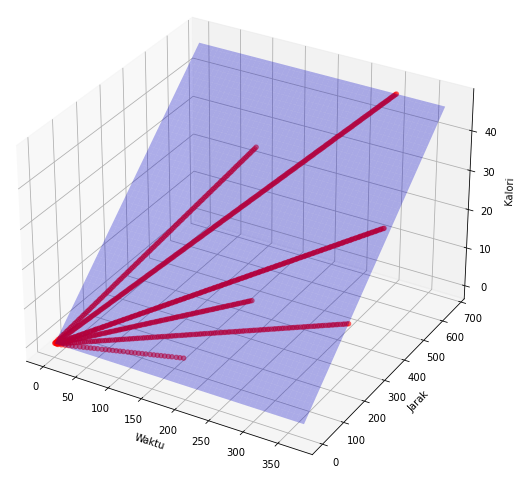
\includegraphics[scale=0.6]{gambar/model regresi kalori3.png}
  \caption{Model regresi linear prediksi kalori terbakar}
  \label{fig:ModelRegresiKalori}
\end{figure}

Tahap selanjutnya setelah mendapatkan model regresi linear untuk prediksi kalori terbakar adalah perhitungan banyak langkah berdasarkan dataset yang telah dibuat dengan mengamati perhitungan langkah dari data video sebenarnya. Data banyak langkah ini akan digunakan sebagai acuan dalam menentukan panjang langkah yang dihasilkan dari tiap variasi yang dilakukan. Dalam melangkah seseorang akan menghasilkan panjang langkah yang berbeda berdasarkan kecepatan yang dilakukan. Panjang langkah ini akan digunakan sebagai pengali dari data akuisisi berupa banyak langkah untuk nantinya dapat menghasilkan jarak tempuh yang dilakukan. Untuk menentukan panjang langkah yang didapat berdasarkan data jarak tempuh dan banyak langkah yang ditempuh dapat dengan menggunakan konversi persamaan yang ditunjukkan pada Persamaan \ref{eq:KonversiPanjangLangkah}.

\begin{equation}
  \label{eq:KonversiPanjangLangkah}
  Panjang Langkah = \frac{Jarak Tempuh}{Banyak Langkah}
\end{equation}

Proses perhitungan banyak langkah dari data video yang digunakan disimpan menjadi dataset untuk selanjutnya dilakukan pengolahan data. Hasil dataset perhitungan banyak langkah juga dilanjutkan dengan perhitungan panjang langkah dari setiap variasi dataset. Proses ini dilakukan untuk membuat dataset yang nantinya akan digunakan untuk melakukan prediksi terhadap panjang langkah saat melakukan estimasi pose dan deteksi langkah. Prediksi panjang langkah ini digunakan sebelum melakukan proses prediksi kalori terbakar saat melakukan akuisisi data dan prediksi kalori terbakar untuk mendapatkan data jarak tempuh yang kemudian digunakan untuk melakukan prediksi kalori terbakar. Tabel \ref{tb:OlahDatasetPanjang} menunjukkan hasil pengolahan data untuk dataset panjang langkah yang akan dilakukan pada proses prediksi panjang langkah.

\begin{longtable}{|c|c|c|c|}
  \caption{Hasil pengolahan data pada dataset panjang langkah}
  \label{tb:OlahDatasetPanjang}                                   \\
  \hline
  \rowcolor[HTML]{C0C0C0}
  \textbf{No} & \textbf{Waktu (detik)} & \textbf{Langkah} & \textbf{Panjang Langkah} \\
  \hline
  1   & 6    & 4    & 0.38089      \\
  \hline
  2   & 11    & 8    & 0.38089     \\
  \hline
  54   & 50    & 53    & 0.52057     \\
  \hline
  55   & 53    & 57    & 0.52057     \\
  \hline
  215   & 63    & 85    & 0.61583     \\
  \hline
  216   & 65    & 88    & 0.61583     \\
  \hline
  375   & 78    & 131    & 0.66120     \\
  \hline
  376   & 79    & 133    & 0.66120     \\
  \hline
  700   & 103    & 263    & 0.86869     \\
  \hline
  701   & 104    & 266    & 0.86869     \\
  \hline
  1044   & 146    & 385    & 1.26289     \\
  \hline
  1045   & 147    & 388    & 1.26289     \\
  \hline
\end{longtable}

Hasil pengolahan data untuk dataset panjang langkah digunakan untuk membuat model regresi polinomial dalam menentukan prediksi panjang langkah. Model regresi polinomial dibuat berdasarkan data berupa waktu dalam detik, langkah dan panjang langkah. Pembagian data dilakukan berdasarkan variabel dalam membuat model regresi polinomial yaitu variabel independen dan variabel dependen. Variabel independen mencakup data mengenai waktu dan langkah, sedangkan variabel dependen merupakan data panjang langkah. Tabel \ref{tb:VariabelPrediksiPanjang} menunjukkan pembagian dataset berdasarkan variabel untuk model regresi yang akan dilakukan.

\begin{longtable}{|c|c|c|}
  \caption{Pembagian dataset panjang langkah berdsarkan variabel regresi}
  \label{tb:VariabelPrediksiPanjang}                                   \\
  \hline
  \rowcolor[HTML]{C0C0C0}
  \multicolumn{2}{|c|}{\textbf{Variabel Independen}}  & \textbf{Variabel Dependen}  \\
  \hline
  \rowcolor[HTML]{C0C0C0}
  \textbf{Waktu (detik)} & \textbf{Jarak Tempuh (meter)} & \textbf{Kalori Terbakar} \\
  \hline
  6    & 4    & 0.38089      \\
  \hline
  11    & 8    & 0.38089     \\
  \hline
  50    & 53    & 0.52057     \\
  \hline
  53    & 57    & 0.52057     \\
  \hline
  63    & 85    & 0.61583     \\
  \hline
  65    & 88    & 0.61583     \\
  \hline
  78    & 131    & 0.66120     \\
  \hline
  79    & 133    & 0.66120     \\
  \hline
  103    & 263    & 0.86869     \\
  \hline
  104    & 266    & 0.86869     \\
  \hline
  146    & 385    & 1.26289     \\
  \hline
  147    & 388    & 1.26289     \\
  \hline
\end{longtable}

Model regresi polinomial dibuat berdasarkan pembagian dataset sesuai variabel yang digunakan. Hasil dari model regresi polinomial berupa persamaan regresi polinomial yang akan digunakan dalam proses prediksi selanjutnya. Dataset yang telah dibagi dilakukan prose pembuatan model menghasilkan proyeksi model regresi berdasarkan data dan persamaan regresi polinomial yang digunakan. Hasil proyeksi dari model regresi polinomial untuk prediksi panjang langkah yang didapatkan ditunjukkan pada Gambar \ref{fig:ModelRegresiPanjang}.

\begin{figure}[H]
  \centering
  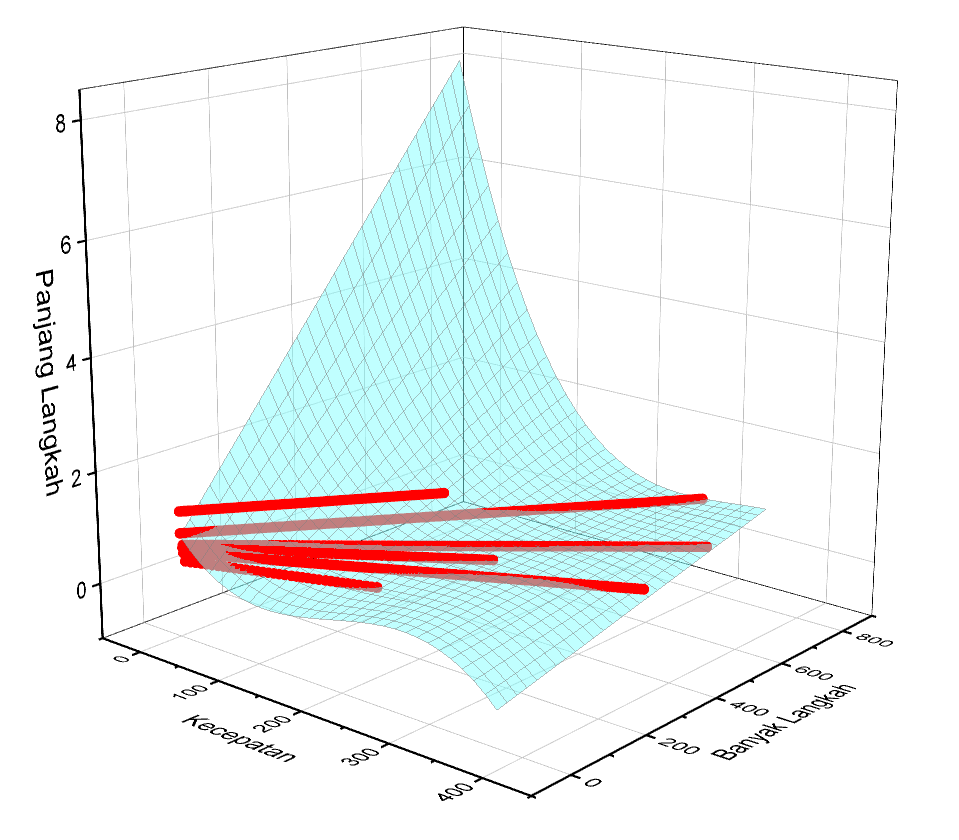
\includegraphics[scale=0.4]{gambar/model regresi panjang.png}
  \caption{Model regresi polinomial prediksi panjang langkah}
  \label{fig:ModelRegresiPanjang}
\end{figure}

Setelah pengolahan data dan model telah dilakukan dapat dilanjutkan dengan melakukan proses prediksi kalori yang terbakar dengan regresi linear. Proses melakukan prediksi dapat dilakukan dengan melakukan akuisisi data dengan data video atau menggunakan pengambilan data secara langsung. Data video kemudian dilanjutkan dengan proses estimasi pose untuk mendapatkan beberapa data gambar yang akan digunakan untuk proses klasifikasi dengan model deteksi langkah. Saat klasifikasi akan menghasilkan data yang nantinya akan digunakan untuk prediksi kalori. Hasil klasifikasi berupa data banyak langkah dan waktu tempuh. Data hasil klasifikasi akan diproses untuk dicari panjang langkah dengan model regresi polinomial untuk prediksi panjang langkah. Hasil prediksi akan digunakan untuk melakukan perhitungan terhadap banyak akumulasi langkah dikalikan dengan prediksi panjang langkah untuk menghasilkan jarak tempuh. Setelah didapatkan jarak tempuh dan waktu tempuh saat akuisisi data sudah dilakukan akan dilanjutkan dengan prediksi kalori menggunakan model regresi linear untuk prediksi kalori terbakar. Hasil prediksi kalori terbakar akan didapatkan berdasarkan model yang sudah dibuat dan data yang didapat.

\subsection{Perhitungan Rumus}
\label{subsec:PrediksiPerhitungan}

Perhitungan kalori dilakukan dengan mengacu pada nilai satuan ukuran \emph{(Metabolic Equivalent of Task)} (MET). Satuan MET akan mendapat pengukuran untuk konsumsi oksigen dan pembakaran kalori. Nilai dari satuan MET dapat didefinisikan pada Persamaan \ref{eq:SatuanMET}.

\begin{equation}
  \label{eq:SatuanMET}
  1 \mathbf{MET} = 3,5 ml O_2  / KG / min
\end{equation}

Berdasarkan nilai satuan ukuran MET, didapatkan suatu persamaan untuk menghitung pembakaran kalori yang didefiniskan pada Persamaan \ref{eq:RumusKalori}.

\begin{equation}
  \label{eq:RumusKalori}
  \mathbf{Cal} = \frac{MET  x 3.5 x BB}{200} x \frac{duration}{60} calories / min
\end{equation}

Pada persamaan pembakaran kalori yang akan digunakan untuk melakukan perhitungan pembakaran kalori dari aktivitas yang dilakukan dibutuhkan beberapa nilai variabel untuk mendapatkah hasil total pembakaran kalori, yaitu nilai MET, nilai berat badan (BB), dan nilai waktu tempuh dalam menit.

Setiap aktivitas memiliki nilai MET yang berbeda-beda dan telah ditentukan oleh peneliti yang telah merangkum banyak aktivitas untuk ditentukan berapa nilai MET yang dihasilkan. Pada aktivitas olahraga yang difokuskan saat ini adalah jogging pada treadmill juga memiliki perbedaan nilai MET yang dipengaruhi oleh kecepatan jogging. Dataset MET terkait aktivitas olaharga terhadap jogging didapatkan untuk digunakan dalam prediksi kalori terbakar menggunakan perhitungan rumus pada penelitian ini. Terdapat data variasi kecepatan yang memiliki nilai MET yang bervariasi. Tabel \ref{tb:DatasetMET} menunjukkan dataset yang digunakan sebagai acuan dalam menentukan kecepatan dan MET yang didapat untuk kemudian dilakukan proses prediksi kalori terbakar.

\begin{longtable}{|c|c|}
  \caption{Dataset pengaruh kecepatan terhadap MET}
  \label{tb:DatasetMET}                                   \\
  \hline
  \rowcolor[HTML]{C0C0C0}
  \textbf{Kecepatan (km/j)} & \textbf{MET}  \\
  \hline
  6.43738  & 6    \\
  \hline
  8.04672   & 8.3    \\
  \hline
  8.36859   & 9    \\
  \hline
  9.65606   & 9.8    \\
  \hline
  10.7826   & 10.5    \\
  \hline
  11.2654   & 11    \\
  \hline
  12.0701   & 11.8    \\
  \hline
  12.8748   & 11.8    \\
  \hline
  13.8404   & 12.3    \\
  \hline
  14.4841   & 12.8    \\
  \hline
  16.0934   & 14.5    \\
  \hline
  17.7028   & 16    \\
  \hline
  19.3121   & 19    \\
  \hline
  20.9215   & 19.8    \\
  \hline
  22.5308   & 23    \\
  \hline
\end{longtable}

Dataset MET yang didapat menunjukkan jika nilai MET dapat diketahui dengan berdasarkan kecepatan yang dilakukan saat melakukan aktivitas olahraga \emph{jogging}. Berdasarkan hasil deteksi pada sistem yang digunakan pada penelitian ini untuk melakukan prediksi kalori berupa jumlah langkah dan waktu tempuh yang kemudian dilakukan pengolahan data untuk menghasilkan data jarak tempuh dan waktu tempuh dapat dilakukan pengolahan lanjut untuk mencari kecepatan tempuh. Kecepatan tempuh dapat kemudian dilakukan pengolahan kembali untuk mencari nilai MET dan melakukan prediksi kalori terbakar dengan menggunakan rumus. Untuk mencari kecepatan tempuh dapat diketahui dengan nilai hasil deteksi dan pengolahan data berupa jarak tempuh dan waktu tempuh untuk menentukan kecepatan tempuh dengan menggunakan Persamaan \ref{eq:RumusKecepatan}.

\begin{equation}
  \label{eq:RumusKecepatan}
  Kecepatan = \frac{Jarak}{Waktu}
\end{equation}

Berdasarkan dataset kecepatan untuk mengetahui MET dapat kemudian dilakukan pembuatan model regresi linear untuk dapat menentukan prediksi MET berdasarkan hasil deteksi dengan pengolahan berupa data kecepatan. Model regresi linear dibuat berdasarkan data berupa kecepatan dan MET. Pembagian data dilakukan berdasarkan variabel dalam membuat model regresi linear yaitu variabel independen dan variabel dependen. Variabel independen meliputi data kecepatan dan variabel dependen meliputi data MET. Tabel \ref{tb:VariabelPrediksiMET} menunjukkan pembagian dataset berdasarkan variabel untuk model regresi yang akan dilakukan.

\begin{longtable}{|c|c|}
  \caption{Pembagian dataset MET berdasarkan variabel regresi}
  \label{tb:VariabelPrediksiMET}                                   \\
  \hline
  \rowcolor[HTML]{C0C0C0}
  \textbf{Variabel Independen}  & \textbf{Variabel Dependen}  \\
  \hline
  \rowcolor[HTML]{C0C0C0}
  \textbf{Kecepatan (km/j)} & \textbf{MET}  \\
  \hline
  6.43738  & 6    \\
  \hline
  8.04672   & 8.3    \\
  \hline
  8.36859   & 9    \\
  \hline
  9.65606   & 9.8    \\
  \hline
  10.7826   & 10.5    \\
  \hline
  11.2654   & 11    \\
  \hline
  12.0701   & 11.8    \\
  \hline
  12.8748   & 11.8    \\
  \hline
  13.8404   & 12.3    \\
  \hline
  14.4841   & 12.8    \\
  \hline
  16.0934   & 14.5    \\
  \hline
  17.7028   & 16    \\
  \hline
  19.3121   & 19    \\
  \hline
  20.9215   & 19.8    \\
  \hline
  22.5308   & 23    \\
  \hline
\end{longtable}

Model regresi linear dibuat berdasarkan pembagian dataset sesuai variabel yang digunakan. Hasil dari model regresi linear berupa persamaan regresi linear yang akan digunakan dalam proses prediksi selanjutnya. Dataset yang telah dibagi dilakukan prose pembuatan model menghasilkan proyeksi model regresi berdasarkan data dan persamaan regresi linear yang digunakan. Hasil proyeksi dari model regresi linear untuk prediksi MET yang didapatkan ditunjukkan pada Gambar \ref{fig:ModelRegresiMET}.

\begin{figure}[H]
  \centering
  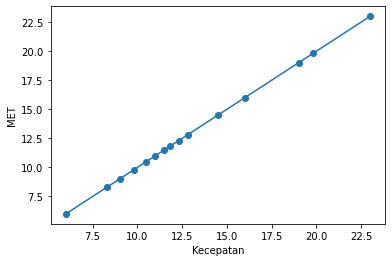
\includegraphics[scale=0.8]{gambar/model regresi met.png}
  \caption{Model regresi linear prediksi MET}
  \label{fig:ModelRegresiMET}
\end{figure}

Setelah pengolahan data dan model telah dilakukan dapat dilanjutkan dengan melakukan proses prediksi kalori yang terbakar dengan perhitungan rumus. Proses melakukan prediksi dapat dilakukan dengan melakukan akuisisi data dengan data video atau menggunakan pengambilan data secara langsung. Data video kemudian dilanjutkan dengan proses estimasi pose untuk mendapatkan beberapa data gambar yang akan digunakan untuk proses klasifikasi dengan model deteksi langkah. Saat klasifikasi akan menghasilkan data yang nantinya akan digunakan untuk prediksi kalori. Hasil klasifikasi berupa data banyak langkah dan waktu tempuh. Data hasil klasifikasi akan diproses untuk dicari panjang langkah dengan model regresi polinomial untuk prediksi panjang langkah. Hasil prediksi akan digunakan untuk melakukan perhitungan terhadap banyak akumulasi langkah dikalikan dengan prediksi panjang langkah untuk menghasilkan jarak tempuh. Setelah didapatkan jarak tempuh dan waktu tempuh saat akuisisi data sudah dilakukan akan dilanjutkan dengan pengolahan data dari hasil deteksi jarak tempuh dan waktu tempuh untuk diketahui kecepatan tempuh berdasarkan konversi pada pengolahan data. Kecepatan tempuh yang didapat akan dilakukan prediksi MET menggunakan model regresi linear untuk prediksi MET. Hasil MET yang didapat akan dilakukan perhitungan menggunakan perhitungan rumus berdasarkan MET untuk kemudian menggunakan data waktu tempuh dan variabel berat badan (BB) sebesar 70 sebagai ukuran standar. Perhitungan rumus yang dilakukan berdasarkan nilai-nilai variabel yang telah ditentukan dalam proses merupakan hasil akhir berupa prediksi kalori yang terbakar.

\cleardoublepage

% Bab 4 pengujian dan analisis
\chapter{PENGUJIAN DAN ANALISIS}
\label{chap:pengujiananalisis}

% Ubah bagian-bagian berikut dengan isi dari pengujian dan analisis

Penelitian dilakukan dengan melakukan uji dan anaisa dari sistem yang telah dibuat berdasarkan langkah pada metodologi yang telah dilaksanakan. Pengujian ini dilakukan untuk menguji kemampuan sistem yang telah dibuat dalam menjawab permasalahan yang dijadikan acuan pada penelitian ini untuk mendapatkan hasil dari tujuan yang ingin didapat. Pembahasan pengujian yang dilakukan pada penelitian ini meliputi pengujian hasil \emph{training} dan \emph{validation} model, pengujian hasil \emph{testing} model, pengujian hasil deteksi dan pengujian prediksi.

\section{Pengujian Hasil \emph{Ttraining} dan \emph{Validation} Model}
\label{sec:PengujianTrainingValidation}

Pengujian pembuatan model berdasarkan hasil \emph{training} dan \emph{validation} dengan menggunakan dataset dengan jumlah keseluruhan yaitu 1731 sampel data. Dengan jumlah sample training sebanyak 1385 dan sampel validation sebanyak 346. Setelah dilakukan proses \emph{training} dan \emph{validation} terhadap dataset yang telah ditentukan oleh sampel data, didapatkan hasil pengujian akurasi dengan tingkat akurasi training sebesar 96\% dan tingkat akurasi validation sebesar 96\%. Kemudian didapatkan hasil pengujian loss pada training sebesar 0,4\% dan loss pada validation sebesar 0,4\%. Hasil pengujian ditunjukkan pada grafik nilai akurasi dan loss pada proses \emph{training} dan \emph{validation} seperti pada Gambar \ref{fig:HasilTrainingValidation}.

\begin{figure}[H]
  \centering
  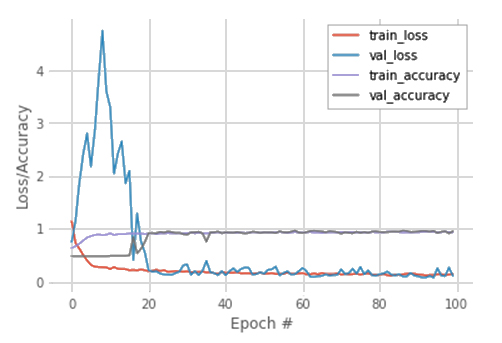
\includegraphics[scale=0.65]{gambar/hasil training dan validation w.jpg}
  \caption{Grafik hasil \emph{training} dan \emph{validation}}
  \label{fig:HasilTrainingValidation}
\end{figure}


\section{Pengujian Testing Model}
\label{sec:PengujianTestingModel}

Pengujian dilanjutkan dengan melakukan \emph{testing} model dengan menggunakan dataset yang sudah dimiliki dengan jumlah keseluruhan yaitu 347 sampel data. Dataset yang digunakan merupakan dataset yang sudah dilakukan filtrasi yang hanya digunakan pada pengujian \emph{testing} saja. Hasil pengujian \emph{testing} model didapatkan akurasi sebesar 95\% dengan hasil deteksi benar untuk kelas kanan sebanyak 170 sampel 96\% dan kelas kiri sebanyak 161 sampel 95\%. Pengujian ditunjukkan dengan confusion matrix pada Gambar \ref{fig:HasilTesting} dan Tabel \ref{tb:ClassificationReport} merupakan classification report dari hasil pengujian yang telah dilakukan pada pengujian \emph{testing} model penelitian ini.

\begin{figure}[H]
  \centering
  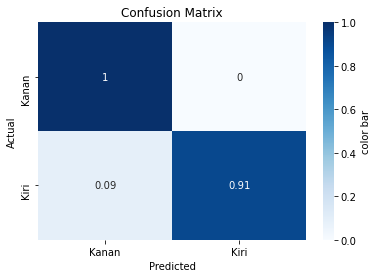
\includegraphics[scale=1]{gambar/cm normalized.png}
  \caption{\emph{Confusion Matrix} hasil \emph{testing} model}
  \label{fig:HasilTesting}
\end{figure}

\begin{longtable}{|c|c|c|c|c|}
  \caption{\emph{Classification Report} hasil pengujian \emph{testing} model}
  \label{tb:ClassificationReport}                                   \\
  \hline
  \rowcolor[HTML]{C0C0C0}
   & \textbf{Precision} & \textbf{Recall} & \textbf{F1-Score} & \textbf{Support} \\
  \hline
  kanan     & 0,91    & 1,00    & 0,96    & 170         \\
  \hline
  kiri      & 1,00    & 0,91    & 0,95    & 177           \\
  \hline
  Accuracy  &         &         & 0,95    & 347            \\
  \hline
\end{longtable}

\section{Pengujian Hasil Deteksi}
\label{sec:PengujianDeteksi}

Proses deteksi yang dilakukan dengan menggunakan model yang telah dibuat dilakukan pengujian dari hasil yang didapat dari hasil deteksi dengan perhitungan yang sebenarnya. Pengujian dilakukan dengan membuat data sebenarnya dengan melakukan perhitungan langkah dari akuisisi maupun data video yang digunakan dalam percobaan dan dibandingkan dengan hasil perhitungan langkah dari hasil deteksi. Tabel \ref{tb:PengujianDeteksi} menunjukkan hasil perhitungan data sebenarnya dengan data hasil deteksi terhadap langkah pada data video. 

\begin{longtable}{|c|c|c|}
  \caption{Pengujian Hasil Deteksi}
  \label{tb:PengujianDeteksi}                                   \\
  \hline
  \rowcolor[HTML]{C0C0C0}
  \textbf{Percobaan} & \textbf{Langkah} & \textbf{Deteksi Langkah} \\
  \hline
  1   & 241   & 328    \\
  \hline
  2   & 169   & 170    \\
  \hline
  3   & 302   & 302    \\
  \hline
  4   & 246   & 248    \\
  \hline
  5   & 321   & 322    \\
  \hline
  6   & 220   & 218    \\
  \hline
\end{longtable}

Pengujian dilakukan setelah didapatkan data hasil deteksi yang telah didapat dan juga data sebenarnya berdasarkan hasil perhitungan yang dilakukan terhadap data video. Setiap percobaan dilakukan analisa terkait perbandingan hasil yang didapat antara data hasil deteksi dan data perhitungan sebenarnya. Perbandingan dilakukan dengan mencari nilai error dari hasil perbedaan yang didapat dan dikalkulasikan dalam hasil akurasi dan error yang didapat dari analisa tersebut. Hasil analisa yang didapat dengan melakukan analisa pengujian hasil deteksi didapatkan hasil akurasi sebesar 99,36\% dengan hasil error sebesar 0,64\%. Tabel \ref{tb:AnalisaDeteksi} menunjukkan hasil analisa dari setiap percobaan yang dilakukan analisa pengujian.

\begin{longtable}{|c|c|c|c|c|c|}
  \caption{Analisa Pengujian Hasil Deteksi}
  \label{tb:AnalisaDeteksi}                                   \\
  \hline
  \rowcolor[HTML]{C0C0C0}
  \textbf{Percobaan} & \textbf{Langkah} & \textbf{Deteksi Langkah} & \textbf{Error} & \textbf{Error\%} & \textbf{Akurasi\%} \\
  \hline
  1   & 241   & 328 & 3   & 1,24\%    & 98,76\%   \\
  \hline
  2   & 169   & 170 & 1   & 0,59\%    & 99,41\%   \\
  \hline
  3   & 302   & 302 & 0   & 0\%       & 100\%     \\
  \hline
  4   & 246   & 248 & 2   & 0,81\%    & 99,19\%   \\
  \hline
  5   & 321   & 322 & 1   & 0,31\%    & 99,69\%   \\
  \hline
  6   & 220   & 218 & 2   & 0,91\%    & 99,09\%   \\
  \hline
\end{longtable}


\section{Pengujian Prediksi}
\label{sec:PengujianPrediksi}

Pengujian pada prediksi jumlah kalori yang terbakar dilakukan setelah melakukan pengujian pada model deteksi yang telah dilakukan. Prediksi dilakukan dengan dua metode, yaitu regresi linear dan perhitungan rumus. Dengan menggunakan dataset berupa citra video yang akan digunakan untuk melakukan prediksi kalori sebanyak 6 sampel video sehingga terdapat 6 percobaan yang dilakukan. Pada pengujian dengan regresi linear dengan melakukan proses deteksi dan menggunakan model regresi linear dalam melakukan proses prediksi kalori didapatkan beberapa data pendukung dalam hasil deteksi dan data dari hasil regresi prediksi kalori. Tabel \ref{tb:PengujianPrediksiRegresi} menunjukkan hasil deteksi dan hasil prediksi kalori dengan menggunakan regresi linear.

\begin{longtable}{|c|c|c|c|c|}
  \caption{Pengujian Prediksi dengan Regresi Linear}
  \label{tb:PengujianPrediksiRegresi}                                   \\
  \hline
  \rowcolor[HTML]{C0C0C0}
  \textbf{Percobaan} & \textbf{Deteksi Langkah} & \textbf{Jarak} & \textbf{Waktu} & \textbf{Kalori} \\
  \hline
  1   & 238   & 167,181    & 2:50    & 11,652  \\
  \hline
  2   & 170   & 118,437    & 1:35    & 8,245   \\
  \hline
  3   & 302   & 293,143    & 2:02    & 20,534  \\
  \hline
  4   & 248   & 284,417    & 1:41    & 19,927  \\
  \hline
  5   & 322   & 287,577    & 2:03    & 20,14   \\
  \hline
  6   & 218   & 286,18     & 1:21    & 20,056  \\
  \hline
\end{longtable}

Analisa pengujian \lipsum[1][1-3]. Tabel \ref{tb:AnalisaPrediksiRegresi} menunjukkan hasil analisa pengujian dari prediksi kalori dengan regresi linear.

\begin{longtable}{|c|c|c|c|c|c|}
  \caption{Analisa Pengujian Prediksi dengan Regresi Linear}
  \label{tb:AnalisaPrediksiRegresi}                                   \\
  \hline
  \rowcolor[HTML]{C0C0C0}
  \textbf{Percobaan} & \textbf{Kalori Treadmill} & \textbf{Prediksi Kalori} & \textbf{Error} & \textbf{Error\%} & \textbf{Akurasi\%} \\
  \hline
  1   & 10   & 11,652   & 1,652    & 16,52\%     & 83,48\%   \\
  \hline
  2   & 10   & 8,245    & 1,755    & 17,55\%     & 82,45\%   \\
  \hline
  3   & 20   & 20,534   & 0,534    & 2,67\%      & 97,33\%   \\
  \hline
  4   & 20   & 19,927   & 0,073    & 0,365\%     & 99,635\%  \\
  \hline
  5   & 20   & 20,14    & 0,14     & 0,7\%       & 99,3\%    \\
  \hline
  6   & 20   & 20,056   & 0,056    & 0,28\%      & 99,72\%   \\
  \hline
\end{longtable}

Pada pengujian dengan perhitungan rumus berdasarkan MET dilakukan dengan melalui proses deteksi dan melakukan perhitungan rumus menghasilkan beberapa data pendukung dalam perhitungan rumus dan hasil prediksi kalori yang didapat. Tabel \ref{tb:PengujianPrediksiPerhitungan} menunjukkan hasil deteksi dan hasil prediksi kalori dengan menggunakan perhitungan rumus.

\begin{longtable}{|c|c|c|c|c|}
  \caption{Pengujian Prediksi dengan Perhitungan Rumus}
  \label{tb:PengujianPrediksiPerhitungan}                                   \\
  \hline
  \rowcolor[HTML]{C0C0C0}
  \textbf{Percobaan} & \textbf{Deteksi Kecepatan} & \textbf{MET} & \textbf{Waktu} & \textbf{Kalori} \\
  \hline
  1   & 3,626   & 2,003    & 2:50    & 6,788   \\
  \hline
  2   & 5,016   & 2,733    & 1:35    & 4.744   \\
  \hline
  3   & 8,943   & 9,323    & 2:02    & 22.462  \\
  \hline
  4   & 10,893  & 10,721   & 1:41    & 20.575  \\
  \hline
  5   & 8,151   & 8,533    & 2:03    & 22.126  \\
  \hline
  6   & 13,041  & 11,985   & 1:21    & 19.331  \\
  \hline
\end{longtable}

Analisa pengujian \lipsum[1][1-4]. Tabel \ref{tb:AnalisaPrediksiPerhitungan} menunjukkan hasil analisa pengujian dari prediksi kalori dengan perhitungan rumus.

\begin{longtable}{|c|c|c|c|c|c|}
  \caption{Analisa Pengujian Prediksi dengan Perhitungan Rumus}
  \label{tb:AnalisaPrediksiPerhitungan}                                   \\
  \hline
  \rowcolor[HTML]{C0C0C0}
  \textbf{Percobaan} & \textbf{Kalori Treadmill} & \textbf{Prediksi Kalori} & \textbf{Error} & \textbf{Error\%} & \textbf{Akurasi\%} \\
  \hline
  1   & 10   & 6,788 & 3,212    & 32,12\%     & 67,88\%   \\
  \hline
  2   & 10   & 4,744 & 5,251    & 52,56\%     & 47,44\%   \\
  \hline
  3   & 20   & 22,462 & 2,462   & 12,31\%     & 87,69\%   \\
  \hline
  4   & 20   & 20,575 & 0,575   & 2,86\%      & 91,14\%   \\
  \hline
  5   & 20   & 22,126 & 2,126   & 10,63\%     & 89,37\%   \\
  \hline
  6   & 20   & 19,311 & 0,669   & 3,35\%      & 96,65\%   \\
  \hline
\end{longtable}

Hasil yang diperoleh melalui model yang telah dibuat untuk deteksi dan melakukan prediksi sesuai metode yang dilakukan didapatkan hasil akumulasi kalori dengan prediksi regresi sebesar 93,61\% dengan akumulasi error sebesar 6,39\%. Kemudian prediksi dengan perhitungan rumus didapatkan hasil akumulasi akurasi kalori sebesar 81,03\% dengan akumulasi error sebesar 18,97\%. Tabel \ref{tb:PengujianPrediksi} merupakan hasil perbandingan antara dataset percobaan dengan nilai kalori pembanding dataset dengan proses prediksi.

\begin{longtable}{|c|c|c|c|c|}
  \caption{Pengujian Hasil Prediksi Kalori}
  \label{tb:PengujianPrediksi}                                   \\
  \hline
  \rowcolor[HTML]{C0C0C0}
  \textbf{Percobaan} & \textbf{Kecepatan} & \textbf{Kalori Treadmill} & \textbf{Prediksi Regresi} & \textbf{Perhitungan MET} \\
  \hline
  1   & 3     & 10    & 11,652    & 6,788   \\
  \hline
  2   & 6     & 10    & 8,245     & 4,744   \\
  \hline
  3   & 9     & 20    & 20,534    & 22,462   \\
  \hline
  4   & 12    & 20    & 19,927    & 20,575   \\
  \hline
  5   & 8     & 20    & 20,14     & 22,126   \\
  \hline
  6   & 12    & 20    & 20,056    & 19,331   \\
  \hline
\end{longtable}
\cleardoublepage

% Bab 5 penutup
\chapter{PENUTUP}
\label{chap:penutup}

% Ubah bagian-bagian berikut dengan isi dari penutup

\section{Kesimpulan}
\label{sec:kesimpulan}

Berdasarkan hasil pengujian yang \lipsum[1][1-3] sebagai berikut:

\begin{enumerate}[nolistsep]

  \item Pembuatan \lipsum[2][1-3]

  \item \lipsum[2][4-6]

  \item \lipsum[2][7-10]

\end{enumerate}

\section{Saran}
\label{chap:saran}

Untuk pengembangan lebih lanjut pada \lipsum[1][1-3] antara lain:

\begin{enumerate}[nolistsep]

  \item Memperbaiki \lipsum[2][1-3]

  \item \lipsum[2][4-6]

  \item \lipsum[2][7-10]

\end{enumerate}

\cleardoublepage

\chapter*{DAFTAR PUSTAKA}
\addcontentsline{toc}{chapter}{DAFTAR PUSTAKA}

\begingroup
%\renewcommand{\section}[2]{}%
\renewcommand{\chapter}[2]{}% for other classes
\begin{thebibliography}{}
  \bibitem{ano05}
    World Health Organization. (2022). Noncommunicable diseases: progress monitor 2022. World Health Organization. https://apps.who.int/iris/handle/10665/353048. License: CC BY-NC-SA 3.0 IGO
 \bibitem{ano05}
    Blüher, M. (2019). Obesity: global epidemiology and pathogenesis. Nature Reviews Endocrinology. doi:10.1038/s41574-019-0176-8
 \bibitem{ano05}
    World Health Organization. (2022). Global status report on physical activity 2022. World Health Organization. https://apps.who.int/iris/handle/10665/363607. License: CC BY-NC-SA 3.0 IGO
 \bibitem{ano05}
    Caballero, Y., Ando, T. J., Nakae, S., Usui, C., Aoyama, T., Nakanishi, M., … Tanaka, S. (2019). Simple Prediction of Metabolic Equivalents of Daily Activities Using Heart Rate Monitor without Calibration of Individuals. International Journal of Environmental Research and Public Health, 17(1), 216. doi:10.3390/ijerph17010216
 \bibitem{ano05}
    Safaei, M., Sundararajan, E. A., Driss, M., Boulila, W., \& Shapi’i, A. (2021). A systematic literature review on obesity: Understanding the causes \& consequences of obesity and reviewing various machine learning approaches used to predict obesity. Computers in Biology and Medicine, 136, 104754. doi:10.1016/j.compbiomed.2021.104754 
 \bibitem{ano05}
    Bohlen, A., Boll, M., Schwarzer, M., \& Groneberg, D. A. (2014). Body-Mass-Index. Zentralblatt Für Arbeitsmedizin, Arbeitsschutz Und Ergonomie, 64(6), 415–429. doi:10.1007/s40664-014-0074-9
 \bibitem{ano05}
    Lobstein, T. et al., 2023. World Obesity Atlas 2023, World Obesity Federation. United Kingdom.
 \bibitem{ano05}
    Kevin D Hall and others, The energy balance model of obesity: beyond calories in, calories out, The American Journal of Clinical Nutrition, Volume 115, Issue 5, May 2022, Pages 1243–1254, https://doi.org/10.1093/ajcn/nqac031
 \bibitem{ano05}
    Anderson, E., \& Durstine, J. L. (2019). Physical Activity, Exercise, and Chronic Diseases: A Brief Review. Sports Medicine and Health Science. doi:10.1016/j.smhs.2019.08.006
 \bibitem{ano05}
    Erkkola, R. U., Vasankari, T., \& Erkola, A. (2020). Opinion paper: Exercise for healthy aging. Maturitas. doi:10.1016/j.maturitas.2020.10.012 
 \bibitem{ano05}
    Pojednic, R.; D'Arpino, E.; Halliday, I.; Bantham, A. The Benefits of Physical Activity for People with Obesity, Independent of Weight Loss: A Systematic Review. Int. J. Environ. Res. Public Health 2022, 19, 4981. https://doi.org/10.3390/ijerph19094981
 \bibitem{ano05}
    Marquez, D. X., Aguiñaga, S., Vásquez, P. M., Conroy, D. E., Erickson, K. I., Hillman, C., … Powell, K. E. (2020). A systematic review of physical activity and quality of life and well-being. Translational Behavioral Medicine, 10(5), 1098–1109. doi:10.1093/tbm/ibz198
 \bibitem{ano05}
    Gaesser, Glenn \& Angadi, Siddhartha. (2021). Obesity treatment: Weight loss versus increasing fitness and physical activity for reducing health risks. iScience. 24. 10.1016/j.isci.2021.102995.
 \bibitem{ano05}
    Nurhayati, Faridha \& Wahjuni, Endang \& Andrijanto, Dony \& Febriyanti, Irma \& Kaharina, Arifah. (2020). Quality of Life and Level of Physical Activity in Sports Education Students During the COVID-19 Pandemic. 10.2991/assehr.k.201201.196.
  \bibitem{ano05}
    Okmayura, F., Effendi, N., Ramadhani, W., Jefiza, A. (2019). Analysis and Design of Calories Burning Calculation in Jogging Using Thresholding Based Accelerometer Sensor. Advances in Engineering Research, vol 190. https://doi.org/10.2991/iccelst-st-19.2019.3
  \bibitem{oe04}
    Utami, D., B. dan Ichwan, M. (2017). Sistem Prediksi Kalori Terbakar Pada Pesepeda Menggunakan Feedforward Neural Network. https:// https://lib.itenas.ac.id/kti/?p=5185
  \bibitem{oe04}
    Saponaro, P., Wei, H., Dominick, G., Kambhamettu, C. (2019). Estimating Physical Activity Intensity And Energy Expenditure Using Computer Vision On Videos. https://doi.org/10.1109/ICIP.2019.8803535
  \bibitem{oe04}
    P. Ilmiah, M. Ajidarma, P. S. Informatika, F. Komunikasi, D. A. N. Informatika, and U. M. Surakarta. (2019). Aplikasi perhitungan kebutuhan kalori dan perhitungan kalori dari makanan yang dikonsumsi.
  \bibitem{oe04}
    F. T. Informasi. (2016). Pengembangan Sistem Monitoring Aktivitas Fisik User Bergerak dengan Analisa Langkah ( Step Analysis ) untuk Estimasi Pembakaran Kalori secara Real-Time.
  \bibitem{oe04}
    W. Widiantini et al. 2013. Aktivitas Fisik , Stres , dan Obesitas pada Pegawai Negeri Sipil Physical Activity , Stress and Obesity among Civil Servant, no. 4.
  \bibitem{oe04}
    D. Kurniawan. (2008). Regresi Linier. Statistic, vol. 2, no. 3, pp. 1–6.
  \bibitem{oe04}
    Syilfi, D. S., Ispriyanti, D. (2012). Analsis Regresi. J. Gaussin, vol. 1.
  \bibitem{oe04}
    P. Sulardi, T. Hendro, and F. R. Umbara. (2017). Prediksi Kebutuhan Obat Menggunakan Regresi Linier. Pros. SNATIF, vol. 0, no. 0, pp. 57–62.
  \bibitem{oe04}
    P. Ilmiah, R. D. Nurfita, P. S. Informatika, F. Komunikasi, D. A. N. Informatika, and U. M. Surakarta. (2018). Implementasi Deep Learning Berbasis Tensorflow.
  \bibitem{oe04}
    P. A. Nugroho, I. Fenriana, R. Arijanto, and M. Kom. (2020). Implementasi Deep Learning Menggunakan Convolutional Neural Network ( CNN ) pada Ekspresi Manusia, vol. 1.
  \bibitem{oe04}
    R. Mehindra Prasmatio, B. Rahmat, and I. Yuniar. (2020). Deteksi Dan Pengenalan Ikan Menggunakan Algoritma Convolutional Neural Network.  J. Inform. dan Sist. Inf., vol. 1, no. 2, pp. 510–521.
  \bibitem{oe04}
    H. Fonda. (2020). Klasifikasi Batik Riau Dengan Menggunakan Convolutional Neural Networks (Cnn). J. Ilmu Komput., vol. 9, no. 1, pp. 7–10. doi: 10.33060/jik/2020/vol9.iss1.144.
  \bibitem{oe04}
    W. S. Eka Putra. (2016). Klasifikasi Citra Menggunakan Convolutional Neural Network (CNN) pada Caltech 101. J. Tek. ITS, vol. 5, no. 1, 2016, doi: 10.12962/j23373539.v5i1.15696.
  \bibitem{oe04}
    Theunissen, K., Van Hooren, B., Plasqui, G., \& Meijer, K. (2022). Self-paced and fixed speed treadmill walking yield similar energetics and biomechanics across different speeds. Gait \& posture, 92, 2–7. https://doi.org/10.1016/j.gaitpost.2021.11.005
  \bibitem{oe04}
    Miller, J. R., Van Hooren, B., Bishop, C., Buckley, J. D., Willy, R. W., \& Fuller, J. T. (2019). A Systematic Review and Meta-Analysis of Crossover Studies Comparing Physiological, Perceptual and Performance Measures Between Treadmill and Overground Running. Sports Medicine, 49(5), 763–782. doi:10.1007/s40279-019-01087-9 
  \bibitem{oe04}
    Wiens, C., Denton, W., Schieber, M. N., Hartley, R., Marmelat, V., Myers, S. A., \& Yentes, J. M. (2019). Walking speed and spatiotemporal step mean measures are reliable during feedback-controlled treadmill walking; however, spatiotemporal step variability is not reliable. Journal of Biomechanics. doi:10.1016/j.jbiomech.2018.11.051 
  \bibitem{oe04}
    Ibala, Eunice \& Coupaud, Sylvie \& Kerr, Andy. (2019). Comparison of the Muscle Pattern Variability During Treadmill Walking (Fixed and Self-Pace) and Over Ground Walking of Able-Bodied Adults Journal of Annals of Bioengineering Citation. Journal of Annals of Bioengineering. 1. 1-11. 10.33513/BIOE/1901-04. 
  \bibitem{oe04}
    Nouriani, A., McGovern, R., \& Rajamani, R. (2023). Activity Recognition Using A Combination of High Gain Observer and Deep Learning Computer Vision Algorithms. Intelligent Systems with Applications. Volume 18, ISSN 2667-3053. doi: 10.1016/j.iswa.2023.200213.
  \bibitem{oe04}
    Chai, J., Zeng, H., Li, A., \& Ngai, E. W. T. (2021). Deep learning in computer vision: A critical review of emerging techniques and application scenarios. Machine Learning with Applications, 6, 100134. doi:10.1016/j.mlwa.2021.100134 
  \bibitem{oe04}
    Hou, C. (2020). A study on IMU-Based Human Activity Recognition Using Deep Learning and Traditional Machine Learning. 2020 5th International Conference on Computer and Communication Systems (ICCCS). doi:10.1109/icccs49078.2020.9118506
  \bibitem{oe04}
    Ramanujam, E., Perumal, T., \& Padmavathi, S. (2021). Human Activity Recognition With Smartphone and Wearable Sensors Using Deep Learning Techniques: A Review. IEEE Sensors Journal, 21(12), 13029–13040. doi:10.1109/jsen.2021.3069927 

  \end{thebibliography}
\endgroup

%\renewcommand\refname{}
%\vspace{2ex}
%\renewcommand{\bibname}{}
%\begingroup
%\def\chapter*#1{}
%\printbibliography
%\endgroup
\cleardoublepage

% Biografi penulis
\begin{center}
  \Large
  \textbf{BIOGRAFI PENULIS}
\end{center}

\addcontentsline{toc}{chapter}{BIOGRAFI PENULIS}

\vspace{2ex}

\begin{wrapfigure}{L}{0.3\textwidth}
  \centering
  \vspace{-3ex}
  % Ubah file gambar berikut dengan file foto dari mahasiswa
  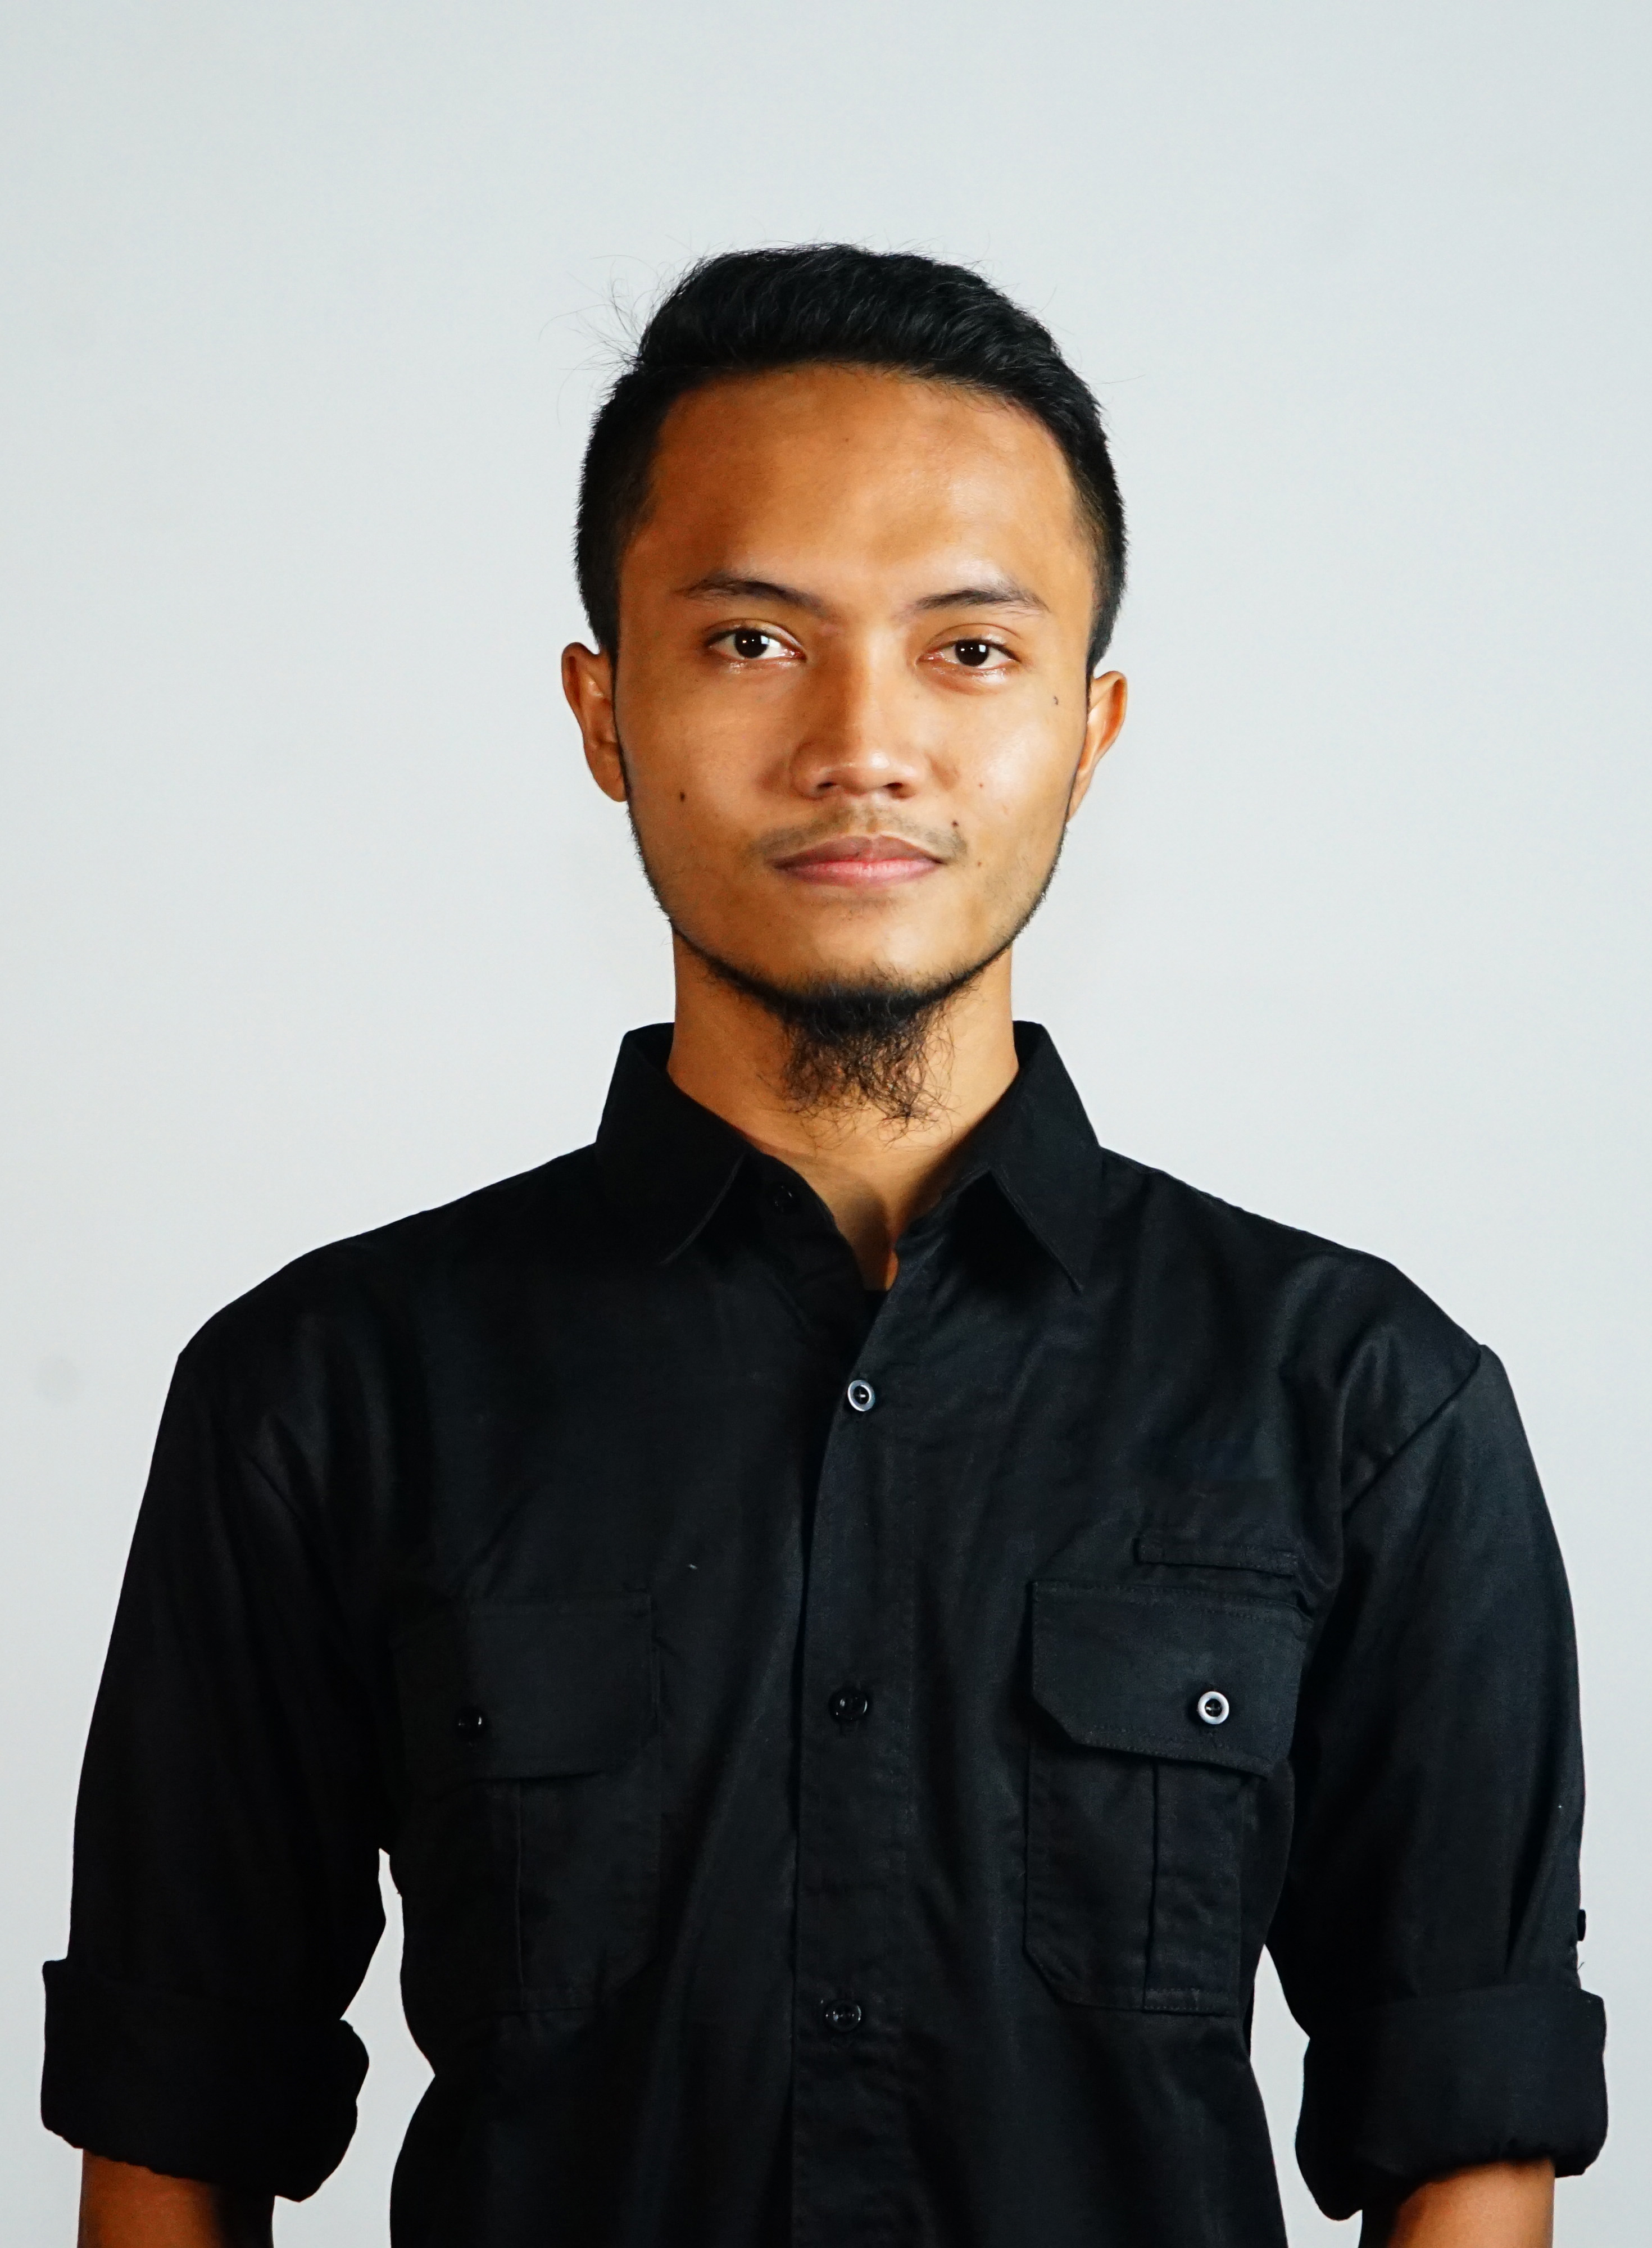
\includegraphics[width=0.3\textwidth]{gambar/biodimas.jpg}
  \vspace{-4ex}
\end{wrapfigure}

% Ubah kalimat berikut dengan biografi dari mahasiswa
\name{}, atau biasa dipanggil Dimas, lahir di Bondowoso, Jawa Timur pada 5 Desember 2000. Merupakan anak kedua dari dua saudara. Penulis lulus dari SMP Negeri 1 Bondowoso dan melanjutkan ke SMA Negeri 2 Bondowoso. Penulis melanjutkan ke jenjang strata satu di Departemen Teknik Komputer Fakultas Teknologi Elektro dan Informatika Cerdas Institut Teknologi Sepuluh Nopember (ITS). Dalam masa kuliah, penulis tertarik dengan jaringan komputer, pengembangan Robotika dan \emph{Internet of Things} (IoT), \emph{Web Design} dan UI/UX. Penulis pernah aktif menjadi salah satu anggota kru hingga menjadi \emph{quality control} dari ITS TV (2020-2023) dan aktif dalam organisasi mahasiswa yaitu anggkota staf Departemen Komunikasi dan Informasi (Kominfo) dan Wakil Departemen \emph{Relation and Comunication} HIMATEKKOM ITS (2021-2023). Pada penelitian akhir ini, penulis memilih mengembangkan penelitian di bidang \emph{Machine Learning} yang berfokus pada Visi Komputer dalam lingkup olahraga pada treadmill. Bagi pembaca yang memiliki kritik, saran, atau pertanyaan mengenai tugas akhir ini dapat menghubungi penulis melalui surel dimas.adityamf@gmail.com.


\cleardoublepage

\end{document}
